\documentclass[twoside]{book}

% Packages required by doxygen
\usepackage{fixltx2e}
\usepackage{calc}
\usepackage{doxygen}
\usepackage[export]{adjustbox} % also loads graphicx
\usepackage{graphicx}
\usepackage[utf8]{inputenc}
\usepackage{makeidx}
\usepackage{multicol}
\usepackage{multirow}
\PassOptionsToPackage{warn}{textcomp}
\usepackage{textcomp}
\usepackage[nointegrals]{wasysym}
\usepackage[table]{xcolor}

% Font selection
\usepackage[T1]{fontenc}
\usepackage[scaled=.90]{helvet}
\usepackage{courier}
\usepackage{amssymb}
\usepackage{sectsty}
\renewcommand{\familydefault}{\sfdefault}
\allsectionsfont{%
  \fontseries{bc}\selectfont%
  \color{darkgray}%
}
\renewcommand{\DoxyLabelFont}{%
  \fontseries{bc}\selectfont%
  \color{darkgray}%
}
\newcommand{\+}{\discretionary{\mbox{\scriptsize$\hookleftarrow$}}{}{}}

% Page & text layout
\usepackage{geometry}
\geometry{%
  a4paper,%
  top=2.5cm,%
  bottom=2.5cm,%
  left=2.5cm,%
  right=2.5cm%
}
\tolerance=750
\hfuzz=15pt
\hbadness=750
\setlength{\emergencystretch}{15pt}
\setlength{\parindent}{0cm}
\setlength{\parskip}{3ex plus 2ex minus 2ex}
\makeatletter
\renewcommand{\paragraph}{%
  \@startsection{paragraph}{4}{0ex}{-1.0ex}{1.0ex}{%
    \normalfont\normalsize\bfseries\SS@parafont%
  }%
}
\renewcommand{\subparagraph}{%
  \@startsection{subparagraph}{5}{0ex}{-1.0ex}{1.0ex}{%
    \normalfont\normalsize\bfseries\SS@subparafont%
  }%
}
\makeatother

% Headers & footers
\usepackage{fancyhdr}
\pagestyle{fancyplain}
\fancyhead[LE]{\fancyplain{}{\bfseries\thepage}}
\fancyhead[CE]{\fancyplain{}{}}
\fancyhead[RE]{\fancyplain{}{\bfseries\leftmark}}
\fancyhead[LO]{\fancyplain{}{\bfseries\rightmark}}
\fancyhead[CO]{\fancyplain{}{}}
\fancyhead[RO]{\fancyplain{}{\bfseries\thepage}}
\fancyfoot[LE]{\fancyplain{}{}}
\fancyfoot[CE]{\fancyplain{}{}}
\fancyfoot[RE]{\fancyplain{}{\bfseries\scriptsize Generated by Doxygen }}
\fancyfoot[LO]{\fancyplain{}{\bfseries\scriptsize Generated by Doxygen }}
\fancyfoot[CO]{\fancyplain{}{}}
\fancyfoot[RO]{\fancyplain{}{}}
\renewcommand{\footrulewidth}{0.4pt}
\renewcommand{\chaptermark}[1]{%
  \markboth{#1}{}%
}
\renewcommand{\sectionmark}[1]{%
  \markright{\thesection\ #1}%
}

% Indices & bibliography
\usepackage{natbib}
\usepackage[titles]{tocloft}
\setcounter{tocdepth}{3}
\setcounter{secnumdepth}{5}
\makeindex

% Hyperlinks (required, but should be loaded last)
\usepackage{ifpdf}
\ifpdf
  \usepackage[pdftex,pagebackref=true]{hyperref}
\else
  \usepackage[ps2pdf,pagebackref=true]{hyperref}
\fi
\hypersetup{%
  colorlinks=true,%
  linkcolor=blue,%
  citecolor=blue,%
  unicode%
}

% Custom commands
\newcommand{\clearemptydoublepage}{%
  \newpage{\pagestyle{empty}\cleardoublepage}%
}

\usepackage{caption}
\captionsetup{labelsep=space,justification=centering,font={bf},singlelinecheck=off,skip=4pt,position=top}

%===== C O N T E N T S =====

\begin{document}

% Titlepage & ToC
\hypersetup{pageanchor=false,
             bookmarksnumbered=true,
             pdfencoding=unicode
            }
\pagenumbering{alph}
\begin{titlepage}
\vspace*{7cm}
\begin{center}%
{\Large Sabina }\\
\vspace*{1cm}
{\large Generated by Doxygen 1.8.13}\\
\end{center}
\end{titlepage}
\clearemptydoublepage
\pagenumbering{roman}
\tableofcontents
\clearemptydoublepage
\pagenumbering{arabic}
\hypersetup{pageanchor=true}

%--- Begin generated contents ---
\chapter{Hierarchical Index}
\section{Class Hierarchy}
This inheritance list is sorted roughly, but not completely, alphabetically\+:\begin{DoxyCompactList}
\item \contentsline{section}{Config\+File}{\pageref{class_config_file}}{}
\item \contentsline{section}{Config\+File\+:\+:file\+\_\+not\+\_\+found}{\pageref{struct_config_file_1_1file__not__found}}{}
\item \contentsline{section}{Plugin\+Instance\+:\+:Impl}{\pageref{class_plugin_instance_1_1_impl}}{}
\item \contentsline{section}{I\+Plugin}{\pageref{class_i_plugin}}{}
\begin{DoxyCompactList}
\item \contentsline{section}{Camera\+\_\+\+Reader}{\pageref{class_camera___reader}}{}
\item \contentsline{section}{Color\+\_\+\+Tracker}{\pageref{class_color___tracker}}{}
\item \contentsline{section}{File\+\_\+\+Writer}{\pageref{class_file___writer}}{}
\item \contentsline{section}{Function\+\_\+\+Caller}{\pageref{class_function___caller}}{}
\item \contentsline{section}{Function\+\_\+\+Test}{\pageref{class_function___test}}{}
\item \contentsline{section}{Joystick\+\_\+\+Writer}{\pageref{class_joystick___writer}}{}
\item \contentsline{section}{Network\+\_\+\+Client}{\pageref{class_network___client}}{}
\item \contentsline{section}{Network\+\_\+\+Server}{\pageref{class_network___server}}{}
\item \contentsline{section}{Screen\+\_\+\+Reader}{\pageref{class_screen___reader}}{}
\item \contentsline{section}{Tuio\+\_\+\+Client}{\pageref{class_tuio___client}}{}
\end{DoxyCompactList}
\item \contentsline{section}{Config\+File\+:\+:key\+\_\+not\+\_\+found}{\pageref{struct_config_file_1_1key__not__found}}{}
\item \contentsline{section}{Plugin\+Factory}{\pageref{class_plugin_factory}}{}
\item \contentsline{section}{Plugin\+Instance}{\pageref{class_plugin_instance}}{}
\item \contentsline{section}{Plugin\+Manager}{\pageref{class_plugin_manager}}{}
\item \contentsline{section}{Screen\+Shot}{\pageref{struct_screen_shot}}{}
\item \contentsline{section}{Shared\+\_\+\+Memory}{\pageref{class_shared___memory}}{}
\item \contentsline{section}{Thread}{\pageref{class_thread}}{}
\item \contentsline{section}{Triplet}{\pageref{struct_triplet}}{}
\item \contentsline{section}{uinput\+\_\+event}{\pageref{structuinput__event}}{}
\item \contentsline{section}{X\+Input\+Joypad}{\pageref{struct_x_input_joypad}}{}
\begin{DoxyCompactList}
\item \contentsline{section}{C\+Joypad}{\pageref{class_c_joypad}}{}
\end{DoxyCompactList}
\end{DoxyCompactList}

\chapter{Class Index}
\section{Class List}
Here are the classes, structs, unions and interfaces with brief descriptions\+:\begin{DoxyCompactList}
\item\contentsline{section}{\hyperlink{class_camera___reader}{Camera\+\_\+\+Reader} \\*\hyperlink{class_camera___reader}{Camera\+\_\+\+Reader} plugin }{\pageref{class_camera___reader}}{}
\item\contentsline{section}{\hyperlink{class_c_joypad}{C\+Joypad} }{\pageref{class_c_joypad}}{}
\item\contentsline{section}{\hyperlink{class_color___tracker}{Color\+\_\+\+Tracker} \\*\hyperlink{class_color___tracker}{Color\+\_\+\+Tracker} plugin }{\pageref{class_color___tracker}}{}
\item\contentsline{section}{\hyperlink{class_config_file}{Config\+File} }{\pageref{class_config_file}}{}
\item\contentsline{section}{\hyperlink{struct_config_file_1_1file__not__found}{Config\+File\+::file\+\_\+not\+\_\+found} }{\pageref{struct_config_file_1_1file__not__found}}{}
\item\contentsline{section}{\hyperlink{class_file___writer}{File\+\_\+\+Writer} \\*\hyperlink{class_file___writer}{File\+\_\+\+Writer} plugin }{\pageref{class_file___writer}}{}
\item\contentsline{section}{\hyperlink{class_function___caller}{Function\+\_\+\+Caller} \\*\hyperlink{class_function___caller}{Function\+\_\+\+Caller} plugin }{\pageref{class_function___caller}}{}
\item\contentsline{section}{\hyperlink{class_function___test}{Function\+\_\+\+Test} \\*\hyperlink{class_function___test}{Function\+\_\+\+Test} plugin }{\pageref{class_function___test}}{}
\item\contentsline{section}{\hyperlink{class_plugin_instance_1_1_impl}{Plugin\+Instance\+::\+Impl} }{\pageref{class_plugin_instance_1_1_impl}}{}
\item\contentsline{section}{\hyperlink{class_i_plugin}{I\+Plugin} }{\pageref{class_i_plugin}}{}
\item\contentsline{section}{\hyperlink{class_joystick___writer}{Joystick\+\_\+\+Writer} \\*\hyperlink{class_joystick___writer}{Joystick\+\_\+\+Writer} plugin }{\pageref{class_joystick___writer}}{}
\item\contentsline{section}{\hyperlink{struct_config_file_1_1key__not__found}{Config\+File\+::key\+\_\+not\+\_\+found} }{\pageref{struct_config_file_1_1key__not__found}}{}
\item\contentsline{section}{\hyperlink{class_network___client}{Network\+\_\+\+Client} \\*\hyperlink{class_network___client}{Network\+\_\+\+Client} plugin }{\pageref{class_network___client}}{}
\item\contentsline{section}{\hyperlink{class_network___server}{Network\+\_\+\+Server} \\*\hyperlink{class_network___server}{Network\+\_\+\+Server} plugin }{\pageref{class_network___server}}{}
\item\contentsline{section}{\hyperlink{class_plugin_factory}{Plugin\+Factory} }{\pageref{class_plugin_factory}}{}
\item\contentsline{section}{\hyperlink{class_plugin_instance}{Plugin\+Instance} \\*C\+O\+R\+E\+\_\+\+A\+PI \hyperlink{class_plugin_instance}{Plugin\+Instance} }{\pageref{class_plugin_instance}}{}
\item\contentsline{section}{\hyperlink{class_plugin_manager}{Plugin\+Manager} \\*C\+O\+R\+E\+\_\+\+A\+PI \hyperlink{class_plugin_manager}{Plugin\+Manager} }{\pageref{class_plugin_manager}}{}
\item\contentsline{section}{\hyperlink{class_screen___reader}{Screen\+\_\+\+Reader} \\*\hyperlink{class_screen___reader}{Screen\+\_\+\+Reader} plugin }{\pageref{class_screen___reader}}{}
\item\contentsline{section}{\hyperlink{struct_screen_shot}{Screen\+Shot} }{\pageref{struct_screen_shot}}{}
\item\contentsline{section}{\hyperlink{class_shared___memory}{Shared\+\_\+\+Memory} }{\pageref{class_shared___memory}}{}
\item\contentsline{section}{\hyperlink{class_thread}{Thread} }{\pageref{class_thread}}{}
\item\contentsline{section}{\hyperlink{struct_triplet}{Triplet} }{\pageref{struct_triplet}}{}
\item\contentsline{section}{\hyperlink{class_tuio___client}{Tuio\+\_\+\+Client} \\*\hyperlink{class_tuio___client}{Tuio\+\_\+\+Client} plugin }{\pageref{class_tuio___client}}{}
\item\contentsline{section}{\hyperlink{structuinput__event}{uinput\+\_\+event} }{\pageref{structuinput__event}}{}
\item\contentsline{section}{\hyperlink{struct_x_input_joypad}{X\+Input\+Joypad} }{\pageref{struct_x_input_joypad}}{}
\end{DoxyCompactList}

\chapter{File Index}
\section{File List}
Here is a list of all documented files with brief descriptions\+:\begin{DoxyCompactList}
\item\contentsline{section}{/home/patrick/projects/\+Gesture\+\_\+\+Therapy\+\_\+\+Linux/src/{\bfseries Main.\+cpp} }{\pageref{_main_8cpp}}{}
\item\contentsline{section}{/home/patrick/projects/\+Gesture\+\_\+\+Therapy\+\_\+\+Linux/src/\+Camera\+\_\+\+Reader/{\bfseries Camera\+\_\+\+Reader.\+h} }{\pageref{_camera___reader_8h}}{}
\item\contentsline{section}{/home/patrick/projects/\+Gesture\+\_\+\+Therapy\+\_\+\+Linux/src/\+Camera\+\_\+\+Reader/{\bfseries dllmain.\+cpp} }{\pageref{_camera___reader_2dllmain_8cpp}}{}
\item\contentsline{section}{/home/patrick/projects/\+Gesture\+\_\+\+Therapy\+\_\+\+Linux/src/\+Camera\+\_\+\+Reader/{\bfseries Main.\+cpp} }{\pageref{_camera___reader_2_main_8cpp}}{}
\item\contentsline{section}{/home/patrick/projects/\+Gesture\+\_\+\+Therapy\+\_\+\+Linux/src/\+Camera\+\_\+\+Reader/{\bfseries tracking.\+hpp} }{\pageref{_camera___reader_2tracking_8hpp}}{}
\item\contentsline{section}{/home/patrick/projects/\+Gesture\+\_\+\+Therapy\+\_\+\+Linux/src/\+Color\+\_\+\+Tracker/{\bfseries Color\+\_\+\+Tracker.\+h} }{\pageref{_color___tracker_8h}}{}
\item\contentsline{section}{/home/patrick/projects/\+Gesture\+\_\+\+Therapy\+\_\+\+Linux/src/\+Color\+\_\+\+Tracker/{\bfseries Main.\+cpp} }{\pageref{_color___tracker_2_main_8cpp}}{}
\item\contentsline{section}{/home/patrick/projects/\+Gesture\+\_\+\+Therapy\+\_\+\+Linux/src/\+File\+\_\+\+Writer/{\bfseries File\+\_\+\+Writer.\+h} }{\pageref{_file___writer_8h}}{}
\item\contentsline{section}{/home/patrick/projects/\+Gesture\+\_\+\+Therapy\+\_\+\+Linux/src/\+File\+\_\+\+Writer/{\bfseries Main.\+cpp} }{\pageref{_file___writer_2_main_8cpp}}{}
\item\contentsline{section}{/home/patrick/projects/\+Gesture\+\_\+\+Therapy\+\_\+\+Linux/src/\+Function\+\_\+\+Caller/{\bfseries Function\+\_\+\+Caller.\+h} }{\pageref{_function___caller_8h}}{}
\item\contentsline{section}{/home/patrick/projects/\+Gesture\+\_\+\+Therapy\+\_\+\+Linux/src/\+Function\+\_\+\+Caller/{\bfseries Main.\+cpp} }{\pageref{_function___caller_2_main_8cpp}}{}
\item\contentsline{section}{/home/patrick/projects/\+Gesture\+\_\+\+Therapy\+\_\+\+Linux/src/\+Function\+\_\+\+Test/{\bfseries Function\+\_\+\+Test.\+h} }{\pageref{_function___test_8h}}{}
\item\contentsline{section}{/home/patrick/projects/\+Gesture\+\_\+\+Therapy\+\_\+\+Linux/src/\+Function\+\_\+\+Test/{\bfseries Main.\+cpp} }{\pageref{_function___test_2_main_8cpp}}{}
\item\contentsline{section}{/home/patrick/projects/\+Gesture\+\_\+\+Therapy\+\_\+\+Linux/src/include/{\bfseries Config\+File.\+cpp} }{\pageref{_config_file_8cpp}}{}
\item\contentsline{section}{/home/patrick/projects/\+Gesture\+\_\+\+Therapy\+\_\+\+Linux/src/include/{\bfseries Config\+File.\+h} }{\pageref{_config_file_8h}}{}
\item\contentsline{section}{/home/patrick/projects/\+Gesture\+\_\+\+Therapy\+\_\+\+Linux/src/include/{\bfseries Triplet.\+h} }{\pageref{_triplet_8h}}{}
\item\contentsline{section}{/home/patrick/projects/\+Gesture\+\_\+\+Therapy\+\_\+\+Linux/src/\+Joystick\+\_\+\+Reader/{\bfseries Joypad.\+cpp} }{\pageref{_joypad_8cpp}}{}
\item\contentsline{section}{/home/patrick/projects/\+Gesture\+\_\+\+Therapy\+\_\+\+Linux/src/\+Joystick\+\_\+\+Reader/\hyperlink{_joypad_8h}{Joypad.\+h} \\*This file provides a generic cross platform joypad interface for Win32 \& Linux. Generally the linux implimentation is not as cool as using DirectX, you only really get hold of the values. Using force feedback is beyond Linux at the moment. Oh well.. }{\pageref{_joypad_8h}}{}
\item\contentsline{section}{/home/patrick/projects/\+Gesture\+\_\+\+Therapy\+\_\+\+Linux/src/\+Joystick\+\_\+\+Reader/{\bfseries Main.\+cpp} }{\pageref{_joystick___reader_2_main_8cpp}}{}
\item\contentsline{section}{/home/patrick/projects/\+Gesture\+\_\+\+Therapy\+\_\+\+Linux/src/\+Joystick\+\_\+\+Writer/{\bfseries dllmain.\+cpp} }{\pageref{_joystick___writer_2dllmain_8cpp}}{}
\item\contentsline{section}{/home/patrick/projects/\+Gesture\+\_\+\+Therapy\+\_\+\+Linux/src/\+Joystick\+\_\+\+Writer/{\bfseries Joystick\+\_\+\+Writer.\+h} }{\pageref{_joystick___writer_8h}}{}
\item\contentsline{section}{/home/patrick/projects/\+Gesture\+\_\+\+Therapy\+\_\+\+Linux/src/\+Joystick\+\_\+\+Writer/{\bfseries Main.\+cpp} }{\pageref{_joystick___writer_2_main_8cpp}}{}
\item\contentsline{section}{/home/patrick/projects/\+Gesture\+\_\+\+Therapy\+\_\+\+Linux/src/\+Network\+\_\+\+Client/{\bfseries Main.\+cpp} }{\pageref{_network___client_2_main_8cpp}}{}
\item\contentsline{section}{/home/patrick/projects/\+Gesture\+\_\+\+Therapy\+\_\+\+Linux/src/\+Network\+\_\+\+Server/{\bfseries Main.\+cpp} }{\pageref{_network___server_2_main_8cpp}}{}
\item\contentsline{section}{/home/patrick/projects/\+Gesture\+\_\+\+Therapy\+\_\+\+Linux/src/\+Plugin\+\_\+\+A\+P\+I/{\bfseries coreapi.\+cpp} }{\pageref{coreapi_8cpp}}{}
\item\contentsline{section}{/home/patrick/projects/\+Gesture\+\_\+\+Therapy\+\_\+\+Linux/src/\+Plugin\+\_\+\+A\+P\+I/\hyperlink{coreapi_8h}{coreapi.\+h} \\*A factory object to create Renderer instances }{\pageref{coreapi_8h}}{}
\item\contentsline{section}{/home/patrick/projects/\+Gesture\+\_\+\+Therapy\+\_\+\+Linux/src/\+Plugin\+\_\+\+A\+P\+I/\hyperlink{defines_8h}{defines.\+h} \\*Win32 decorator macros for the Core and Plugin A\+P\+Is }{\pageref{defines_8h}}{}
\item\contentsline{section}{/home/patrick/projects/\+Gesture\+\_\+\+Therapy\+\_\+\+Linux/src/\+Plugin\+\_\+\+A\+P\+I/\hyperlink{plugin_8h}{plugin.\+h} }{\pageref{plugin_8h}}{}
\item\contentsline{section}{/home/patrick/projects/\+Gesture\+\_\+\+Therapy\+\_\+\+Linux/src/\+Plugin\+\_\+\+A\+P\+I/{\bfseries pluginapi.\+cpp} }{\pageref{pluginapi_8cpp}}{}
\item\contentsline{section}{/home/patrick/projects/\+Gesture\+\_\+\+Therapy\+\_\+\+Linux/src/\+Plugin\+\_\+\+A\+P\+I/\hyperlink{pluginapi_8h}{pluginapi.\+h} \\*An A\+PI that lets users write plugins }{\pageref{pluginapi_8h}}{}
\item\contentsline{section}{/home/patrick/projects/\+Gesture\+\_\+\+Therapy\+\_\+\+Linux/src/\+Plugin\+\_\+\+A\+P\+I/{\bfseries pluginmanager.\+cpp} }{\pageref{pluginmanager_8cpp}}{}
\item\contentsline{section}{/home/patrick/projects/\+Gesture\+\_\+\+Therapy\+\_\+\+Linux/src/\+Plugin\+\_\+\+A\+P\+I/\hyperlink{pluginmanager_8h}{pluginmanager.\+h} \\*A Plugin Manager singleton }{\pageref{pluginmanager_8h}}{}
\item\contentsline{section}{/home/patrick/projects/\+Gesture\+\_\+\+Therapy\+\_\+\+Linux/src/\+Plugin\+\_\+\+A\+P\+I/{\bfseries thread.\+cpp} }{\pageref{thread_8cpp}}{}
\item\contentsline{section}{/home/patrick/projects/\+Gesture\+\_\+\+Therapy\+\_\+\+Linux/src/\+Plugin\+\_\+\+A\+P\+I/{\bfseries thread.\+h} }{\pageref{thread_8h}}{}
\item\contentsline{section}{/home/patrick/projects/\+Gesture\+\_\+\+Therapy\+\_\+\+Linux/src/\+Screen\+\_\+\+Reader/{\bfseries dllmain.\+cpp} }{\pageref{_screen___reader_2dllmain_8cpp}}{}
\item\contentsline{section}{/home/patrick/projects/\+Gesture\+\_\+\+Therapy\+\_\+\+Linux/src/\+Screen\+\_\+\+Reader/{\bfseries Main.\+cpp} }{\pageref{_screen___reader_2_main_8cpp}}{}
\item\contentsline{section}{/home/patrick/projects/\+Gesture\+\_\+\+Therapy\+\_\+\+Linux/src/\+Screen\+\_\+\+Reader/{\bfseries tracking.\+hpp} }{\pageref{_screen___reader_2tracking_8hpp}}{}
\item\contentsline{section}{/home/patrick/projects/\+Gesture\+\_\+\+Therapy\+\_\+\+Linux/src/\+Shared\+\_\+\+Memory/{\bfseries dllmain.\+cpp} }{\pageref{_shared___memory_2dllmain_8cpp}}{}
\item\contentsline{section}{/home/patrick/projects/\+Gesture\+\_\+\+Therapy\+\_\+\+Linux/src/\+Shared\+\_\+\+Memory/{\bfseries Shared\+\_\+\+Memory.\+cpp} }{\pageref{_shared___memory_8cpp}}{}
\item\contentsline{section}{/home/patrick/projects/\+Gesture\+\_\+\+Therapy\+\_\+\+Linux/src/\+Shared\+\_\+\+Memory/{\bfseries Shared\+\_\+\+Memory.\+h} }{\pageref{_shared___memory_8h}}{}
\item\contentsline{section}{/home/patrick/projects/\+Gesture\+\_\+\+Therapy\+\_\+\+Linux/src/\+Tuio\+\_\+\+Client/{\bfseries Main.\+cpp} }{\pageref{_tuio___client_2_main_8cpp}}{}
\end{DoxyCompactList}

\chapter{Class Documentation}
\hypertarget{class_camera___reader}{}\section{Camera\+\_\+\+Reader Class Reference}
\label{class_camera___reader}\index{Camera\+\_\+\+Reader@{Camera\+\_\+\+Reader}}


\hyperlink{class_camera___reader}{Camera\+\_\+\+Reader} plugin.  




{\ttfamily \#include $<$Camera\+\_\+\+Reader.\+h$>$}



Inheritance diagram for Camera\+\_\+\+Reader\+:\nopagebreak
\begin{figure}[H]
\begin{center}
\leavevmode
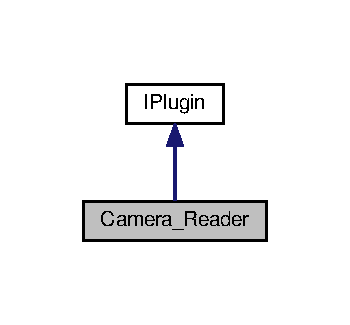
\includegraphics[width=168pt]{class_camera___reader__inherit__graph}
\end{center}
\end{figure}


Collaboration diagram for Camera\+\_\+\+Reader\+:\nopagebreak
\begin{figure}[H]
\begin{center}
\leavevmode
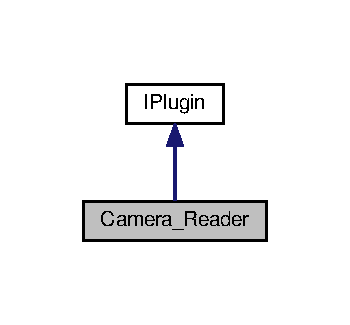
\includegraphics[width=168pt]{class_camera___reader__coll__graph}
\end{center}
\end{figure}
\subsection*{Public Member Functions}
\begin{DoxyCompactItemize}
\item 
void \hyperlink{class_camera___reader_af3fabc94e27e6ce1702d26829126b9dc}{Main} ()
\begin{DoxyCompactList}\small\item\em Main funcction of the plugin. \end{DoxyCompactList}\item 
bool \hyperlink{class_camera___reader_a63163ba2ecf2ff470ca7e6a31dcabfb6}{load\+Configuration} ()
\begin{DoxyCompactList}\small\item\em Load configuration. \end{DoxyCompactList}\item 
bool \hyperlink{class_camera___reader_a3e7d14b675846c5094311985a0c1e735}{save\+Configuration} ()
\begin{DoxyCompactList}\small\item\em Save configuration. \end{DoxyCompactList}\item 
bool \hyperlink{class_camera___reader_a752286c32bea93608d0d23d1d4b3f0ed}{Initialize\+\_\+\+Output} ()
\begin{DoxyCompactList}\small\item\em Initialize Output variables for the plugin to publish. \end{DoxyCompactList}\item 
bool \hyperlink{class_camera___reader_aa4870916d311618a5b6513f12c3e125b}{Initialize\+\_\+\+Input} ()
\begin{DoxyCompactList}\small\item\em Initialize Input variables for the plugin to publish. \end{DoxyCompactList}\item 
void \hyperlink{class_camera___reader_afac6f0a4e2c0df76cad8f1d0d20cdc59}{stop} ()
\begin{DoxyCompactList}\small\item\em Stop plugin. \end{DoxyCompactList}\item 
void \hyperlink{class_camera___reader_a3192d04dc33c238d6f779a72ffc08a5e}{run} ()
\begin{DoxyCompactList}\small\item\em Execute plugin. \end{DoxyCompactList}\end{DoxyCompactItemize}
\subsection*{Additional Inherited Members}


\subsection{Detailed Description}
\hyperlink{class_camera___reader}{Camera\+\_\+\+Reader} plugin. 

This plugin reads the input from the webcam (index 0 unless secefied in config) and publishes it as a cv\+::\+Mat under the name \char`\"{}\+Video\+\_\+\+From\+\_\+\+Camera\char`\"{}

\begin{DoxyAuthor}{Author}
Patrick Heyer, \href{mailto:patrickhey@prodigy.net.mx}{\tt patrickhey@prodigy.\+net.\+mx} 
\end{DoxyAuthor}
\begin{DoxyDate}{Date}
jul 13, 2014 
\end{DoxyDate}
\begin{DoxyVersion}{Version}
1.\+0 
\end{DoxyVersion}


Definition at line 15 of file Camera\+\_\+\+Reader.\+h.



\subsection{Member Function Documentation}
\mbox{\Hypertarget{class_camera___reader_aa4870916d311618a5b6513f12c3e125b}\label{class_camera___reader_aa4870916d311618a5b6513f12c3e125b}} 
\index{Camera\+\_\+\+Reader@{Camera\+\_\+\+Reader}!Initialize\+\_\+\+Input@{Initialize\+\_\+\+Input}}
\index{Initialize\+\_\+\+Input@{Initialize\+\_\+\+Input}!Camera\+\_\+\+Reader@{Camera\+\_\+\+Reader}}
\subsubsection{\texorpdfstring{Initialize\+\_\+\+Input()}{Initialize\_Input()}}
{\footnotesize\ttfamily bool Camera\+\_\+\+Reader\+::\+Initialize\+\_\+\+Input (\begin{DoxyParamCaption}{ }\end{DoxyParamCaption})\hspace{0.3cm}{\ttfamily [virtual]}}



Initialize Input variables for the plugin to publish. 

\begin{DoxyReturn}{Returns}
bool 
\end{DoxyReturn}


Implements \hyperlink{class_i_plugin_aa7c66743ad956d8ada57becee559af4d}{I\+Plugin}.



Definition at line 100 of file Main.\+cpp.


\begin{DoxyCode}
101 \{
102     Plugin\_ERROR = Shared\_Memory::getInstance().Register\_String\_Input(\textcolor{stringliteral}{"Plugin\_ERROR"});
103     \textcolor{keywordflow}{return} \textcolor{keyword}{true};
104 \}
\end{DoxyCode}
\mbox{\Hypertarget{class_camera___reader_a752286c32bea93608d0d23d1d4b3f0ed}\label{class_camera___reader_a752286c32bea93608d0d23d1d4b3f0ed}} 
\index{Camera\+\_\+\+Reader@{Camera\+\_\+\+Reader}!Initialize\+\_\+\+Output@{Initialize\+\_\+\+Output}}
\index{Initialize\+\_\+\+Output@{Initialize\+\_\+\+Output}!Camera\+\_\+\+Reader@{Camera\+\_\+\+Reader}}
\subsubsection{\texorpdfstring{Initialize\+\_\+\+Output()}{Initialize\_Output()}}
{\footnotesize\ttfamily bool Camera\+\_\+\+Reader\+::\+Initialize\+\_\+\+Output (\begin{DoxyParamCaption}{ }\end{DoxyParamCaption})\hspace{0.3cm}{\ttfamily [virtual]}}



Initialize Output variables for the plugin to publish. 

\begin{DoxyReturn}{Returns}
bool 
\end{DoxyReturn}


Implements \hyperlink{class_i_plugin_a0b772513fc8c4ed01240e19c4bb84068}{I\+Plugin}.



Definition at line 93 of file Main.\+cpp.


\begin{DoxyCode}
94 \{   
95 
96     Shared\_Memory::getInstance().Register\_Output(\textcolor{stringliteral}{"Video\_From\_Camera"}, &frame);
97     \textcolor{keywordflow}{return} \textcolor{keyword}{true};
98 \}
\end{DoxyCode}
\mbox{\Hypertarget{class_camera___reader_a63163ba2ecf2ff470ca7e6a31dcabfb6}\label{class_camera___reader_a63163ba2ecf2ff470ca7e6a31dcabfb6}} 
\index{Camera\+\_\+\+Reader@{Camera\+\_\+\+Reader}!load\+Configuration@{load\+Configuration}}
\index{load\+Configuration@{load\+Configuration}!Camera\+\_\+\+Reader@{Camera\+\_\+\+Reader}}
\subsubsection{\texorpdfstring{load\+Configuration()}{loadConfiguration()}}
{\footnotesize\ttfamily bool Camera\+\_\+\+Reader\+::load\+Configuration (\begin{DoxyParamCaption}{ }\end{DoxyParamCaption})\hspace{0.3cm}{\ttfamily [virtual]}}



Load configuration. 

The configuration can be loaded from file, or be hard coded into the plugin (not recomended), initialization of public and private variables should occur here

By default load\+Configuration is called during \hyperlink{class_plugin_manager_a956e653b7db36da9d034b4a93c8308d5}{Plugin\+Manager\+::\+Initialize()} by the plugin manager.

\begin{DoxyReturn}{Returns}
bool 
\end{DoxyReturn}


Implements \hyperlink{class_i_plugin_a418cff309436d3a15d9a4ce7369db6dd}{I\+Plugin}.



Definition at line 70 of file Main.\+cpp.


\begin{DoxyCode}
71 \{
72     std::stringstream path;
73     path <<\textcolor{stringliteral}{"../conf/"} << PLUGIN\_NAME;
74     \hyperlink{class_config_file}{ConfigFile} config( path.str() );
75     config.readInto(Camera\_index, \textcolor{stringliteral}{"Camera\_index"});
76     config.readInto(Visible, \textcolor{stringliteral}{"Visible"});
77     \textcolor{keywordflow}{return} \textcolor{keyword}{true};
78 \}
\end{DoxyCode}
\mbox{\Hypertarget{class_camera___reader_af3fabc94e27e6ce1702d26829126b9dc}\label{class_camera___reader_af3fabc94e27e6ce1702d26829126b9dc}} 
\index{Camera\+\_\+\+Reader@{Camera\+\_\+\+Reader}!Main@{Main}}
\index{Main@{Main}!Camera\+\_\+\+Reader@{Camera\+\_\+\+Reader}}
\subsubsection{\texorpdfstring{Main()}{Main()}}
{\footnotesize\ttfamily void Camera\+\_\+\+Reader\+::\+Main (\begin{DoxyParamCaption}{ }\end{DoxyParamCaption})\hspace{0.3cm}{\ttfamily [virtual]}}



Main funcction of the plugin. 

Started in a new thread by the Run() funcction is the most importatn funcction of the plugin. Infinite loop (generaly a while(running) function that runs undefenitly in a read/process/write cicle). \begin{DoxyReturn}{Returns}
void 
\end{DoxyReturn}


Implements \hyperlink{class_i_plugin_ab5fdb3b0f7afdcee04324dca01766749}{I\+Plugin}.



Definition at line 37 of file Main.\+cpp.


\begin{DoxyCode}
38 \{
39 
40 
41     cap.open(Camera\_index); 
42     \textcolor{keywordflow}{if} (!cap.isOpened())  \textcolor{comment}{// if not success, exit program}
43     \{
44         LOG(ERROR) << \textcolor{stringliteral}{"Can not open the web cam"};
45         *Plugin\_ERROR = \textcolor{stringliteral}{"NO\_CAMERA"};
46         \textcolor{keywordflow}{return};
47     \}
48     LOG(TRACE) << \textcolor{stringliteral}{"Web cam connected"};
49         
50     \textcolor{keywordflow}{while} (running)
51     \{
52         \textcolor{keywordtype}{double} tic = (double)cvGetTickCount();
53         \textcolor{keywordtype}{bool} bSuccess = cap.read(frame\_from\_cam); \textcolor{comment}{// read a new frame from video}
54 
55         \textcolor{keywordflow}{if} (!bSuccess) \textcolor{comment}{//if not success, break loop}
56         \{
57             LOG(WARNING) << \textcolor{stringliteral}{"Cannot read a frame from video stream"};
58         \}
59         \textcolor{keywordflow}{else} 
60         \{
61             \textcolor{keywordflow}{if}(Visible==1)
62             imshow(\textcolor{stringliteral}{"Cam"}, frame\_from\_cam);          
63         \}
64     \}
65     cap.release();
66     stoped = \textcolor{keyword}{true};
67     \textcolor{keywordflow}{return};
68 \}
\end{DoxyCode}
\mbox{\Hypertarget{class_camera___reader_a3192d04dc33c238d6f779a72ffc08a5e}\label{class_camera___reader_a3192d04dc33c238d6f779a72ffc08a5e}} 
\index{Camera\+\_\+\+Reader@{Camera\+\_\+\+Reader}!run@{run}}
\index{run@{run}!Camera\+\_\+\+Reader@{Camera\+\_\+\+Reader}}
\subsubsection{\texorpdfstring{run()}{run()}}
{\footnotesize\ttfamily void Camera\+\_\+\+Reader\+::run (\begin{DoxyParamCaption}{ }\end{DoxyParamCaption})\hspace{0.3cm}{\ttfamily [virtual]}}



Execute plugin. 

Starts a new thread and executes the plugins main() funcction. \begin{DoxyReturn}{Returns}
void 
\end{DoxyReturn}


Implements \hyperlink{class_i_plugin_a46b4ace767e77f9db9c9585e99c09039}{I\+Plugin}.



Definition at line 106 of file Main.\+cpp.



References I\+Plugin\+::\+Inc\+Wrapper().


\begin{DoxyCode}
107 \{
108     pthread\_create(&thread\_id, NULL, &\hyperlink{class_i_plugin_a62d22be2fdf66eb7f5c2f797f5f3d7f3}{IPlugin::IncWrapper}, \textcolor{keyword}{this});
109     running = \textcolor{keyword}{true};
110     stoped = \textcolor{keyword}{false};
111 \}
\end{DoxyCode}
\mbox{\Hypertarget{class_camera___reader_a3e7d14b675846c5094311985a0c1e735}\label{class_camera___reader_a3e7d14b675846c5094311985a0c1e735}} 
\index{Camera\+\_\+\+Reader@{Camera\+\_\+\+Reader}!save\+Configuration@{save\+Configuration}}
\index{save\+Configuration@{save\+Configuration}!Camera\+\_\+\+Reader@{Camera\+\_\+\+Reader}}
\subsubsection{\texorpdfstring{save\+Configuration()}{saveConfiguration()}}
{\footnotesize\ttfamily bool Camera\+\_\+\+Reader\+::save\+Configuration (\begin{DoxyParamCaption}{ }\end{DoxyParamCaption})\hspace{0.3cm}{\ttfamily [virtual]}}



Save configuration. 

The configuration should be saved to file, public and private variables that should be configured at startup should be saved.

By default save\+Configuration is called during \hyperlink{class_plugin_manager_ab651a05d6fcb92562807e9f5ecc30855}{Plugin\+Manager\+::\+Unload()} by the plugin manager.

\begin{DoxyReturn}{Returns}
bool 
\end{DoxyReturn}


Implements \hyperlink{class_i_plugin_a79b5c42b1c7b08257a6110b2091039bc}{I\+Plugin}.



Definition at line 80 of file Main.\+cpp.


\begin{DoxyCode}
81 \{
82     std::stringstream path;
83     path <<\textcolor{stringliteral}{"../conf/"} << PLUGIN\_NAME;
84     \hyperlink{class_config_file}{ConfigFile} config( path.str() );
85     config.add(\textcolor{stringliteral}{"Camera\_index"}, Camera\_index);
86     config.add(\textcolor{stringliteral}{"Visible"}, Visible);
87     std::ofstream file(path.str());
88     file << config;
89     file.close();
90     \textcolor{keywordflow}{return} \textcolor{keyword}{true};
91 \}
\end{DoxyCode}
\mbox{\Hypertarget{class_camera___reader_afac6f0a4e2c0df76cad8f1d0d20cdc59}\label{class_camera___reader_afac6f0a4e2c0df76cad8f1d0d20cdc59}} 
\index{Camera\+\_\+\+Reader@{Camera\+\_\+\+Reader}!stop@{stop}}
\index{stop@{stop}!Camera\+\_\+\+Reader@{Camera\+\_\+\+Reader}}
\subsubsection{\texorpdfstring{stop()}{stop()}}
{\footnotesize\ttfamily void Camera\+\_\+\+Reader\+::stop (\begin{DoxyParamCaption}{ }\end{DoxyParamCaption})\hspace{0.3cm}{\ttfamily [virtual]}}



Stop plugin. 

Stops the plugin \begin{DoxyReturn}{Returns}
void 
\end{DoxyReturn}


Implements \hyperlink{class_i_plugin_a86e523c283aec5c9fb21249a76e916ac}{I\+Plugin}.



Definition at line 113 of file Main.\+cpp.


\begin{DoxyCode}
114 \{
115     running = \textcolor{keyword}{false};
116 \}
\end{DoxyCode}


The documentation for this class was generated from the following files\+:\begin{DoxyCompactItemize}
\item 
/home/patrick/projects/\+Gesture\+\_\+\+Therapy\+\_\+\+Linux/src/\+Camera\+\_\+\+Reader/Camera\+\_\+\+Reader.\+h\item 
/home/patrick/projects/\+Gesture\+\_\+\+Therapy\+\_\+\+Linux/src/\+Camera\+\_\+\+Reader/Main.\+cpp\end{DoxyCompactItemize}

\hypertarget{class_c_joypad}{}\section{C\+Joypad Class Reference}
\label{class_c_joypad}\index{C\+Joypad@{C\+Joypad}}


{\ttfamily \#include $<$Joypad.\+h$>$}



Inheritance diagram for C\+Joypad\+:\nopagebreak
\begin{figure}[H]
\begin{center}
\leavevmode
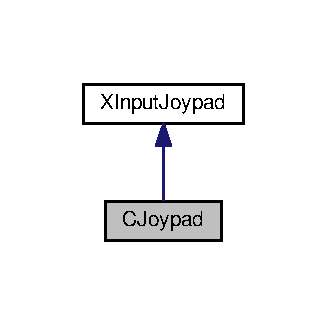
\includegraphics[width=157pt]{class_c_joypad__inherit__graph}
\end{center}
\end{figure}


Collaboration diagram for C\+Joypad\+:\nopagebreak
\begin{figure}[H]
\begin{center}
\leavevmode
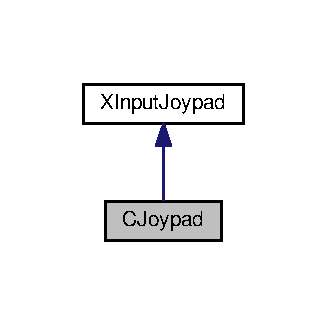
\includegraphics[width=157pt]{class_c_joypad__coll__graph}
\end{center}
\end{figure}
\subsection*{Public Member Functions}
\begin{DoxyCompactItemize}
\item 
\mbox{\Hypertarget{class_c_joypad_adb568eb312a6aeedce38fcac01168887}\label{class_c_joypad_adb568eb312a6aeedce38fcac01168887}} 
const char $\ast$const {\bfseries Instance\+Name} () const
\item 
\mbox{\Hypertarget{class_c_joypad_ac7570ddc23ec4f06d121acc0508525f4}\label{class_c_joypad_ac7570ddc23ec4f06d121acc0508525f4}} 
const char $\ast$const {\bfseries Product\+Name} () const
\item 
const unsigned short \hyperlink{class_c_joypad_ab3a3683d1b12e2071af4751afc2d749c}{Num\+Buttons} () const
\item 
const unsigned short \hyperlink{class_c_joypad_af40e2d5725c3e4d6bdc772e24bb52dca}{Num\+Povs} () const
\item 
bool \hyperlink{class_c_joypad_aad2ba56e14016ef5cd7120b6097caa8c}{HasX} () const
\item 
\mbox{\Hypertarget{class_c_joypad_a3a2f76474de1417ef6ac54c11bca17e1}\label{class_c_joypad_a3a2f76474de1417ef6ac54c11bca17e1}} 
bool {\bfseries HasY} () const
\item 
\mbox{\Hypertarget{class_c_joypad_af7518b10f992af5182eba8e83c803f3a}\label{class_c_joypad_af7518b10f992af5182eba8e83c803f3a}} 
bool {\bfseries HasZ} () const
\item 
\mbox{\Hypertarget{class_c_joypad_a04445b0a73ca1d6da9eb15d0e532b41a}\label{class_c_joypad_a04445b0a73ca1d6da9eb15d0e532b41a}} 
bool {\bfseries Has\+Xrot} () const
\item 
\mbox{\Hypertarget{class_c_joypad_a75ed9276804cd12295d1eafdd7d45c39}\label{class_c_joypad_a75ed9276804cd12295d1eafdd7d45c39}} 
bool {\bfseries Has\+Yrot} () const
\item 
\mbox{\Hypertarget{class_c_joypad_ad5037b8a70da8f60ede0fdaaae3084c7}\label{class_c_joypad_ad5037b8a70da8f60ede0fdaaae3084c7}} 
bool {\bfseries Has\+Zrot} () const
\item 
\mbox{\Hypertarget{class_c_joypad_a684cacc81bfe813f03d19b13b60dcf71}\label{class_c_joypad_a684cacc81bfe813f03d19b13b60dcf71}} 
bool {\bfseries Has\+Extra1} () const
\item 
\mbox{\Hypertarget{class_c_joypad_a4c4b332957d7871a09a214c5d1b04ff7}\label{class_c_joypad_a4c4b332957d7871a09a214c5d1b04ff7}} 
bool {\bfseries Has\+Extra2} () const
\item 
const bool \hyperlink{class_c_joypad_a0125d648a2866c9524e70e3ddeb8b675}{Button} (const unsigned int \&i) const
\item 
\mbox{\Hypertarget{class_c_joypad_a1f707897b1f4d894ced92de429fb9a40}\label{class_c_joypad_a1f707897b1f4d894ced92de429fb9a40}} 
const \hyperlink{_joypad_8h_a2a3e0cda5f1249bef6db47c5eb8e3813}{L\+O\+NG} \hyperlink{class_c_joypad_a1f707897b1f4d894ced92de429fb9a40}{Xaxis} () const
\begin{DoxyCompactList}\small\item\em X-\/axis, usually the left-\/right movement of a stick. \end{DoxyCompactList}\item 
\mbox{\Hypertarget{class_c_joypad_a17e3e401cf2e9dbf42e1f65f3b57e26a}\label{class_c_joypad_a17e3e401cf2e9dbf42e1f65f3b57e26a}} 
const \hyperlink{_joypad_8h_a2a3e0cda5f1249bef6db47c5eb8e3813}{L\+O\+NG} \hyperlink{class_c_joypad_a17e3e401cf2e9dbf42e1f65f3b57e26a}{Xvelocity} () const
\begin{DoxyCompactList}\small\item\em X-\/axis velocity. \end{DoxyCompactList}\item 
\mbox{\Hypertarget{class_c_joypad_a5af5c8672ac198b58276d66ff18aac19}\label{class_c_joypad_a5af5c8672ac198b58276d66ff18aac19}} 
const \hyperlink{_joypad_8h_a2a3e0cda5f1249bef6db47c5eb8e3813}{L\+O\+NG} \hyperlink{class_c_joypad_a5af5c8672ac198b58276d66ff18aac19}{Xacceleration} () const
\begin{DoxyCompactList}\small\item\em X-\/axis acceleration. \end{DoxyCompactList}\item 
\mbox{\Hypertarget{class_c_joypad_af51813f326c05193ff99463d2ac9b969}\label{class_c_joypad_af51813f326c05193ff99463d2ac9b969}} 
const \hyperlink{_joypad_8h_a2a3e0cda5f1249bef6db47c5eb8e3813}{L\+O\+NG} \hyperlink{class_c_joypad_af51813f326c05193ff99463d2ac9b969}{Xforce} () const
\begin{DoxyCompactList}\small\item\em X-\/axis force. \end{DoxyCompactList}\item 
\mbox{\Hypertarget{class_c_joypad_a56189bd2a74dac283c2e2811f3e43598}\label{class_c_joypad_a56189bd2a74dac283c2e2811f3e43598}} 
const \hyperlink{_joypad_8h_a2a3e0cda5f1249bef6db47c5eb8e3813}{L\+O\+NG} \hyperlink{class_c_joypad_a56189bd2a74dac283c2e2811f3e43598}{Yaxis} () const
\begin{DoxyCompactList}\small\item\em Y-\/axis, usually the forward-\/backward movement of a stick. \end{DoxyCompactList}\item 
\mbox{\Hypertarget{class_c_joypad_ac50829aebfc52b28593a3269f35b0a5c}\label{class_c_joypad_ac50829aebfc52b28593a3269f35b0a5c}} 
const \hyperlink{_joypad_8h_a2a3e0cda5f1249bef6db47c5eb8e3813}{L\+O\+NG} \hyperlink{class_c_joypad_ac50829aebfc52b28593a3269f35b0a5c}{Yvelocity} () const
\begin{DoxyCompactList}\small\item\em Y-\/axis velocity. \end{DoxyCompactList}\item 
\mbox{\Hypertarget{class_c_joypad_ab2f6e5d0f3608190036b917787deeb33}\label{class_c_joypad_ab2f6e5d0f3608190036b917787deeb33}} 
const \hyperlink{_joypad_8h_a2a3e0cda5f1249bef6db47c5eb8e3813}{L\+O\+NG} \hyperlink{class_c_joypad_ab2f6e5d0f3608190036b917787deeb33}{Yacceleration} () const
\begin{DoxyCompactList}\small\item\em Y-\/axis acceleration. \end{DoxyCompactList}\item 
\mbox{\Hypertarget{class_c_joypad_a1cceda05c254c0c9e9398cfa4351cac3}\label{class_c_joypad_a1cceda05c254c0c9e9398cfa4351cac3}} 
const \hyperlink{_joypad_8h_a2a3e0cda5f1249bef6db47c5eb8e3813}{L\+O\+NG} \hyperlink{class_c_joypad_a1cceda05c254c0c9e9398cfa4351cac3}{Yforce} () const
\begin{DoxyCompactList}\small\item\em Y-\/axis force. \end{DoxyCompactList}\item 
const \hyperlink{_joypad_8h_a2a3e0cda5f1249bef6db47c5eb8e3813}{L\+O\+NG} \hyperlink{class_c_joypad_a1ab390e90331bc036447eb4fc477e796}{Zaxis} () const
\item 
\mbox{\Hypertarget{class_c_joypad_ac1bdd6e6d030d613bc666797405b8ff6}\label{class_c_joypad_ac1bdd6e6d030d613bc666797405b8ff6}} 
const \hyperlink{_joypad_8h_a2a3e0cda5f1249bef6db47c5eb8e3813}{L\+O\+NG} \hyperlink{class_c_joypad_ac1bdd6e6d030d613bc666797405b8ff6}{Zvelocity} () const
\begin{DoxyCompactList}\small\item\em Z-\/axis velocity. \end{DoxyCompactList}\item 
\mbox{\Hypertarget{class_c_joypad_aa4853aed25405766be055bdb0c7c06a1}\label{class_c_joypad_aa4853aed25405766be055bdb0c7c06a1}} 
const \hyperlink{_joypad_8h_a2a3e0cda5f1249bef6db47c5eb8e3813}{L\+O\+NG} \hyperlink{class_c_joypad_aa4853aed25405766be055bdb0c7c06a1}{Zacceleration} () const
\begin{DoxyCompactList}\small\item\em Z-\/axis acceleration. \end{DoxyCompactList}\item 
\mbox{\Hypertarget{class_c_joypad_a1a1cbce0bc5fe196ae00796ab9355d82}\label{class_c_joypad_a1a1cbce0bc5fe196ae00796ab9355d82}} 
const \hyperlink{_joypad_8h_a2a3e0cda5f1249bef6db47c5eb8e3813}{L\+O\+NG} \hyperlink{class_c_joypad_a1a1cbce0bc5fe196ae00796ab9355d82}{Zforce} () const
\begin{DoxyCompactList}\small\item\em Z-\/axis force. \end{DoxyCompactList}\item 
\mbox{\Hypertarget{class_c_joypad_aff00728a2ebbf208309c3a7849f57596}\label{class_c_joypad_aff00728a2ebbf208309c3a7849f57596}} 
const \hyperlink{_joypad_8h_a2a3e0cda5f1249bef6db47c5eb8e3813}{L\+O\+NG} \hyperlink{class_c_joypad_aff00728a2ebbf208309c3a7849f57596}{Xrot} () const
\begin{DoxyCompactList}\small\item\em X-\/axis rotation. If the joystick does not have this axis, the value is 0. \end{DoxyCompactList}\item 
\mbox{\Hypertarget{class_c_joypad_a76360d49ea28d6232e76b577aca8c72e}\label{class_c_joypad_a76360d49ea28d6232e76b577aca8c72e}} 
const \hyperlink{_joypad_8h_a2a3e0cda5f1249bef6db47c5eb8e3813}{L\+O\+NG} \hyperlink{class_c_joypad_a76360d49ea28d6232e76b577aca8c72e}{Xrot\+Velocity} () const
\begin{DoxyCompactList}\small\item\em X-\/axis angular velocity. \end{DoxyCompactList}\item 
\mbox{\Hypertarget{class_c_joypad_ae90fe74150e87c21916058dafb9c289c}\label{class_c_joypad_ae90fe74150e87c21916058dafb9c289c}} 
const \hyperlink{_joypad_8h_a2a3e0cda5f1249bef6db47c5eb8e3813}{L\+O\+NG} \hyperlink{class_c_joypad_ae90fe74150e87c21916058dafb9c289c}{Xrot\+Acceleration} () const
\begin{DoxyCompactList}\small\item\em X-\/axis angular acceleration. \end{DoxyCompactList}\item 
\mbox{\Hypertarget{class_c_joypad_a1698ee36211a10513530a5bf13558eb9}\label{class_c_joypad_a1698ee36211a10513530a5bf13558eb9}} 
const \hyperlink{_joypad_8h_a2a3e0cda5f1249bef6db47c5eb8e3813}{L\+O\+NG} \hyperlink{class_c_joypad_a1698ee36211a10513530a5bf13558eb9}{Xrot\+Force} () const
\begin{DoxyCompactList}\small\item\em X-\/axis torque. \end{DoxyCompactList}\item 
\mbox{\Hypertarget{class_c_joypad_aa86c6d28e48661188b7e9dd605270ffa}\label{class_c_joypad_aa86c6d28e48661188b7e9dd605270ffa}} 
const \hyperlink{_joypad_8h_a2a3e0cda5f1249bef6db47c5eb8e3813}{L\+O\+NG} \hyperlink{class_c_joypad_aa86c6d28e48661188b7e9dd605270ffa}{Yrot} () const
\begin{DoxyCompactList}\small\item\em Y-\/axis rotation. If the joystick does not have this axis, the value is 0. \end{DoxyCompactList}\item 
\mbox{\Hypertarget{class_c_joypad_a6d65541f2c9059e1c90219bcd3ab8cc4}\label{class_c_joypad_a6d65541f2c9059e1c90219bcd3ab8cc4}} 
const \hyperlink{_joypad_8h_a2a3e0cda5f1249bef6db47c5eb8e3813}{L\+O\+NG} \hyperlink{class_c_joypad_a6d65541f2c9059e1c90219bcd3ab8cc4}{Yrot\+Velocity} () const
\begin{DoxyCompactList}\small\item\em Y-\/axis angular velocity. \end{DoxyCompactList}\item 
\mbox{\Hypertarget{class_c_joypad_abbba1a190c7b6ef552e8dba84969c7fe}\label{class_c_joypad_abbba1a190c7b6ef552e8dba84969c7fe}} 
const \hyperlink{_joypad_8h_a2a3e0cda5f1249bef6db47c5eb8e3813}{L\+O\+NG} \hyperlink{class_c_joypad_abbba1a190c7b6ef552e8dba84969c7fe}{Yrot\+Acceleration} () const
\begin{DoxyCompactList}\small\item\em Y-\/axis angular acceleration. \end{DoxyCompactList}\item 
\mbox{\Hypertarget{class_c_joypad_a769f8470b70666c56444d8eed5ecac10}\label{class_c_joypad_a769f8470b70666c56444d8eed5ecac10}} 
const \hyperlink{_joypad_8h_a2a3e0cda5f1249bef6db47c5eb8e3813}{L\+O\+NG} \hyperlink{class_c_joypad_a769f8470b70666c56444d8eed5ecac10}{Yrot\+Force} () const
\begin{DoxyCompactList}\small\item\em Y-\/axis torque. \end{DoxyCompactList}\item 
const \hyperlink{_joypad_8h_a2a3e0cda5f1249bef6db47c5eb8e3813}{L\+O\+NG} \hyperlink{class_c_joypad_a4cd374af62d1380af4f92156503330a7}{Zrot} () const
\item 
\mbox{\Hypertarget{class_c_joypad_aeac29a2532b14f32b80083732f4e16fc}\label{class_c_joypad_aeac29a2532b14f32b80083732f4e16fc}} 
const \hyperlink{_joypad_8h_a2a3e0cda5f1249bef6db47c5eb8e3813}{L\+O\+NG} \hyperlink{class_c_joypad_aeac29a2532b14f32b80083732f4e16fc}{Zrot\+Velocity} () const
\begin{DoxyCompactList}\small\item\em Z-\/axis angular velocity. . \end{DoxyCompactList}\item 
\mbox{\Hypertarget{class_c_joypad_aabd6bdcfe5e14fe36cc8a18695a5f526}\label{class_c_joypad_aabd6bdcfe5e14fe36cc8a18695a5f526}} 
const \hyperlink{_joypad_8h_a2a3e0cda5f1249bef6db47c5eb8e3813}{L\+O\+NG} \hyperlink{class_c_joypad_aabd6bdcfe5e14fe36cc8a18695a5f526}{Zrot\+Acceleration} () const
\begin{DoxyCompactList}\small\item\em Z-\/axis angular acceleration. \end{DoxyCompactList}\item 
\mbox{\Hypertarget{class_c_joypad_a48fe142d3b2733689c143564ffbcf16a}\label{class_c_joypad_a48fe142d3b2733689c143564ffbcf16a}} 
const \hyperlink{_joypad_8h_a2a3e0cda5f1249bef6db47c5eb8e3813}{L\+O\+NG} \hyperlink{class_c_joypad_a48fe142d3b2733689c143564ffbcf16a}{Zrot\+Force} () const
\begin{DoxyCompactList}\small\item\em Z-\/axis torque. \end{DoxyCompactList}\item 
const \hyperlink{_joypad_8h_a2a3e0cda5f1249bef6db47c5eb8e3813}{L\+O\+NG} \hyperlink{class_c_joypad_ac94bd5a534d97f4c82456397e9a01b1c}{Extra\+Axes} (const unsigned int \&i) const
\item 
\mbox{\Hypertarget{class_c_joypad_a352f2fd69c862c564b2750474b6911ee}\label{class_c_joypad_a352f2fd69c862c564b2750474b6911ee}} 
const \hyperlink{_joypad_8h_a2a3e0cda5f1249bef6db47c5eb8e3813}{L\+O\+NG} {\bfseries Extra\+Velocities} (const unsigned int \&i) const
\item 
\mbox{\Hypertarget{class_c_joypad_aa1770ea6ba770073c43b6b8169aabbba}\label{class_c_joypad_aa1770ea6ba770073c43b6b8169aabbba}} 
const \hyperlink{_joypad_8h_a2a3e0cda5f1249bef6db47c5eb8e3813}{L\+O\+NG} {\bfseries Extra\+Accelerations} (const unsigned int \&i) const
\item 
\mbox{\Hypertarget{class_c_joypad_a705e7a4f1084c37843b23c9d59addcd9}\label{class_c_joypad_a705e7a4f1084c37843b23c9d59addcd9}} 
const \hyperlink{_joypad_8h_a2a3e0cda5f1249bef6db47c5eb8e3813}{L\+O\+NG} {\bfseries Extra\+Forces} (const unsigned int \&i) const
\item 
const D\+W\+O\+RD \hyperlink{class_c_joypad_a52dad2bae4ae8ef1574d963bdd4c1a5d}{P\+OV} (const unsigned int \&i) const
\end{DoxyCompactItemize}
\subsection*{Friends}
\begin{DoxyCompactItemize}
\item 
bool \hyperlink{class_c_joypad_ab38988ebf6ab3808447c491d4f5874e0}{Init\+Input} ()
\begin{DoxyCompactList}\small\item\em Initialize the Direct\+Input variables. \end{DoxyCompactList}\item 
bool \hyperlink{class_c_joypad_a4d5dc1be49e0a6ddee2df5035bc2b56f}{Update\+Input\+State} ()
\begin{DoxyCompactList}\small\item\em You should call this to update the state of the joypad. \end{DoxyCompactList}\item 
\mbox{\Hypertarget{class_c_joypad_abdb51d74a8798e93a46d3149db9d387b}\label{class_c_joypad_abdb51d74a8798e93a46d3149db9d387b}} 
void \hyperlink{class_c_joypad_abdb51d74a8798e93a46d3149db9d387b}{Free\+Input} ()
\begin{DoxyCompactList}\small\item\em Cleans up Direct Input. \end{DoxyCompactList}\end{DoxyCompactItemize}
\subsection*{Additional Inherited Members}


\subsection{Detailed Description}
The Linux implimentation of the joypad interface class. 

Definition at line 588 of file Joypad.\+h.



\subsection{Member Function Documentation}
\mbox{\Hypertarget{class_c_joypad_a0125d648a2866c9524e70e3ddeb8b675}\label{class_c_joypad_a0125d648a2866c9524e70e3ddeb8b675}} 
\index{C\+Joypad@{C\+Joypad}!Button@{Button}}
\index{Button@{Button}!C\+Joypad@{C\+Joypad}}
\subsubsection{\texorpdfstring{Button()}{Button()}}
{\footnotesize\ttfamily const bool C\+Joypad\+::\+Button (\begin{DoxyParamCaption}\item[{const unsigned int \&}]{i }\end{DoxyParamCaption}) const\hspace{0.3cm}{\ttfamily [inline]}, {\ttfamily [virtual]}}

Array of buttons. The high-\/order bit of the byte is set if the corresponding button is down, and clear if the button is up or does not exist. 

Implements \hyperlink{struct_x_input_joypad_a13cc187aae10747b0376cb1ed3710b5a}{X\+Input\+Joypad}.



Definition at line 655 of file Joypad.\+h.


\begin{DoxyCode}
655                                                    \{
656         \textcolor{keywordflow}{return} Buttons[i] != 0;
657     \}
\end{DoxyCode}
\mbox{\Hypertarget{class_c_joypad_ac94bd5a534d97f4c82456397e9a01b1c}\label{class_c_joypad_ac94bd5a534d97f4c82456397e9a01b1c}} 
\index{C\+Joypad@{C\+Joypad}!Extra\+Axes@{Extra\+Axes}}
\index{Extra\+Axes@{Extra\+Axes}!C\+Joypad@{C\+Joypad}}
\subsubsection{\texorpdfstring{Extra\+Axes()}{ExtraAxes()}}
{\footnotesize\ttfamily const \hyperlink{_joypad_8h_a2a3e0cda5f1249bef6db47c5eb8e3813}{L\+O\+NG} C\+Joypad\+::\+Extra\+Axes (\begin{DoxyParamCaption}\item[{const unsigned int \&}]{i }\end{DoxyParamCaption}) const\hspace{0.3cm}{\ttfamily [inline]}, {\ttfamily [virtual]}}

Two additional axis values (formerly called the u-\/axis and v-\/axis) whose semantics depend on the joystick. Use the I\+Direct\+Input\+Device8\+::\+Get\+Object\+Info method to obtain semantic information about these values. 

Implements \hyperlink{struct_x_input_joypad_a074ad76f1e54b559fcee6606049bb6b7}{X\+Input\+Joypad}.



Definition at line 791 of file Joypad.\+h.


\begin{DoxyCode}
791                                                       \{
792         \textcolor{keywordflow}{return} Axes[6+i];
793     \}
\end{DoxyCode}
\mbox{\Hypertarget{class_c_joypad_aad2ba56e14016ef5cd7120b6097caa8c}\label{class_c_joypad_aad2ba56e14016ef5cd7120b6097caa8c}} 
\index{C\+Joypad@{C\+Joypad}!HasX@{HasX}}
\index{HasX@{HasX}!C\+Joypad@{C\+Joypad}}
\subsubsection{\texorpdfstring{Has\+X()}{HasX()}}
{\footnotesize\ttfamily bool C\+Joypad\+::\+HasX (\begin{DoxyParamCaption}{ }\end{DoxyParamCaption}) const\hspace{0.3cm}{\ttfamily [inline]}, {\ttfamily [virtual]}}

the following functions allow you to check to see if the specified axis is available on the joypad. 

Implements \hyperlink{struct_x_input_joypad_a9b5317808345c53bc0df5a3054dd0318}{X\+Input\+Joypad}.



Definition at line 623 of file Joypad.\+h.


\begin{DoxyCode}
623                       \{
624         \textcolor{keywordflow}{return} m\_iAxes>=1;
625     \}
\end{DoxyCode}
\mbox{\Hypertarget{class_c_joypad_ab3a3683d1b12e2071af4751afc2d749c}\label{class_c_joypad_ab3a3683d1b12e2071af4751afc2d749c}} 
\index{C\+Joypad@{C\+Joypad}!Num\+Buttons@{Num\+Buttons}}
\index{Num\+Buttons@{Num\+Buttons}!C\+Joypad@{C\+Joypad}}
\subsubsection{\texorpdfstring{Num\+Buttons()}{NumButtons()}}
{\footnotesize\ttfamily const unsigned short C\+Joypad\+::\+Num\+Buttons (\begin{DoxyParamCaption}{ }\end{DoxyParamCaption}) const\hspace{0.3cm}{\ttfamily [inline]}, {\ttfamily [virtual]}}

this function returns the number of buttons available on the joypad 

Implements \hyperlink{struct_x_input_joypad_a9bc1d9930ca27e815b05542a7fd38a39}{X\+Input\+Joypad}.



Definition at line 607 of file Joypad.\+h.


\begin{DoxyCode}
607                                             \{
608         \textcolor{keywordflow}{return} m\_nButtons;
609     \}
\end{DoxyCode}
\mbox{\Hypertarget{class_c_joypad_af40e2d5725c3e4d6bdc772e24bb52dca}\label{class_c_joypad_af40e2d5725c3e4d6bdc772e24bb52dca}} 
\index{C\+Joypad@{C\+Joypad}!Num\+Povs@{Num\+Povs}}
\index{Num\+Povs@{Num\+Povs}!C\+Joypad@{C\+Joypad}}
\subsubsection{\texorpdfstring{Num\+Povs()}{NumPovs()}}
{\footnotesize\ttfamily const unsigned short C\+Joypad\+::\+Num\+Povs (\begin{DoxyParamCaption}{ }\end{DoxyParamCaption}) const\hspace{0.3cm}{\ttfamily [inline]}, {\ttfamily [virtual]}}

this function returns the number of buttons available on the joypad 

Implements \hyperlink{struct_x_input_joypad_a715b4a23b83fa39ca3940f4e2f45c852}{X\+Input\+Joypad}.



Definition at line 614 of file Joypad.\+h.


\begin{DoxyCode}
614                                          \{
615         \textcolor{keywordflow}{return} 0;
616     \}
\end{DoxyCode}
\mbox{\Hypertarget{class_c_joypad_a52dad2bae4ae8ef1574d963bdd4c1a5d}\label{class_c_joypad_a52dad2bae4ae8ef1574d963bdd4c1a5d}} 
\index{C\+Joypad@{C\+Joypad}!P\+OV@{P\+OV}}
\index{P\+OV@{P\+OV}!C\+Joypad@{C\+Joypad}}
\subsubsection{\texorpdfstring{P\+O\+V()}{POV()}}
{\footnotesize\ttfamily const D\+W\+O\+RD C\+Joypad\+::\+P\+OV (\begin{DoxyParamCaption}\item[{const unsigned int \&}]{i }\end{DoxyParamCaption}) const\hspace{0.3cm}{\ttfamily [inline]}, {\ttfamily [virtual]}}

Direction controllers, such as point-\/of-\/view hats. The position is indicated in hundredths of a degree clockwise from north (away from the user). The center position is normally reported as -\/1; but see Remarks. For indicators that have only five positions, the value for a controller is -\/1, 0, 9,000, 18,000, or 27,000. 

Implements \hyperlink{struct_x_input_joypad_a2f270f296bcaf98089ab23f74a6e9937}{X\+Input\+Joypad}.



Definition at line 815 of file Joypad.\+h.



References Free\+Input(), Init\+Input(), and Update\+Input\+State().


\begin{DoxyCode}
815                                                  \{
816         \textcolor{keywordflow}{return} 0;
817     \}
\end{DoxyCode}
\mbox{\Hypertarget{class_c_joypad_a1ab390e90331bc036447eb4fc477e796}\label{class_c_joypad_a1ab390e90331bc036447eb4fc477e796}} 
\index{C\+Joypad@{C\+Joypad}!Zaxis@{Zaxis}}
\index{Zaxis@{Zaxis}!C\+Joypad@{C\+Joypad}}
\subsubsection{\texorpdfstring{Zaxis()}{Zaxis()}}
{\footnotesize\ttfamily const \hyperlink{_joypad_8h_a2a3e0cda5f1249bef6db47c5eb8e3813}{L\+O\+NG} C\+Joypad\+::\+Zaxis (\begin{DoxyParamCaption}{ }\end{DoxyParamCaption}) const\hspace{0.3cm}{\ttfamily [inline]}, {\ttfamily [virtual]}}

Z-\/axis, often the throttle control. If the joystick does not have this axis, the value is 0. 

Implements \hyperlink{struct_x_input_joypad_af4bfca4d8f22808a92a0ae26468cdedc}{X\+Input\+Joypad}.



Definition at line 706 of file Joypad.\+h.


\begin{DoxyCode}
706                              \{
707         \textcolor{keywordflow}{return} Axes[2];
708     \}
\end{DoxyCode}
\mbox{\Hypertarget{class_c_joypad_a4cd374af62d1380af4f92156503330a7}\label{class_c_joypad_a4cd374af62d1380af4f92156503330a7}} 
\index{C\+Joypad@{C\+Joypad}!Zrot@{Zrot}}
\index{Zrot@{Zrot}!C\+Joypad@{C\+Joypad}}
\subsubsection{\texorpdfstring{Zrot()}{Zrot()}}
{\footnotesize\ttfamily const \hyperlink{_joypad_8h_a2a3e0cda5f1249bef6db47c5eb8e3813}{L\+O\+NG} C\+Joypad\+::\+Zrot (\begin{DoxyParamCaption}{ }\end{DoxyParamCaption}) const\hspace{0.3cm}{\ttfamily [inline]}, {\ttfamily [virtual]}}

Z-\/axis rotation (often called the rudder). If the joystick does not have this axis, the value is 0. 

Implements \hyperlink{struct_x_input_joypad_a4319cae362154a8e069ebe290db8239b}{X\+Input\+Joypad}.



Definition at line 769 of file Joypad.\+h.


\begin{DoxyCode}
769                             \{
770         \textcolor{keywordflow}{return} Axes[5];
771     \}
\end{DoxyCode}


\subsection{Friends And Related Function Documentation}
\mbox{\Hypertarget{class_c_joypad_ab38988ebf6ab3808447c491d4f5874e0}\label{class_c_joypad_ab38988ebf6ab3808447c491d4f5874e0}} 
\index{C\+Joypad@{C\+Joypad}!Init\+Input@{Init\+Input}}
\index{Init\+Input@{Init\+Input}!C\+Joypad@{C\+Joypad}}
\subsubsection{\texorpdfstring{Init\+Input}{InitInput}}
{\footnotesize\ttfamily bool Init\+Input (\begin{DoxyParamCaption}{ }\end{DoxyParamCaption})\hspace{0.3cm}{\ttfamily [friend]}}



Initialize the Direct\+Input variables. 

\begin{DoxyReturn}{Returns}
true if OK

true if OK, false if it fails 
\end{DoxyReturn}


Definition at line 383 of file Joypad.\+cpp.


\begin{DoxyCode}
384 \{
385     \textcolor{keywordtype}{bool} ret=\textcolor{keyword}{false};
386     \textcolor{keywordtype}{int} fd;
387     \textcolor{keywordflow}{if} ( (fd = open(\textcolor{stringliteral}{"/dev/input/js0"}, O\_RDONLY)) > 0 ) 
388     \{
389         \hyperlink{class_c_joypad}{CJoypad}* ptr = \textcolor{keyword}{new} \hyperlink{class_c_joypad}{CJoypad};
390         ioctl(fd, JSIOCGVERSION, &ptr->version);
391         ioctl(fd, JSIOCGAXES, &ptr->m\_iAxes);
392         ioctl(fd, JSIOCGBUTTONS, &ptr->m\_nButtons);
393         ioctl(fd, JSIOCGNAME(NAME\_LENGTH), ptr->name);
394         fcntl(fd, F\_SETFL, O\_NONBLOCK);
395         ptr->fd = fd;
396         g\_aJoypads.push\_back(ptr);
397         ret=\textcolor{keyword}{true};
398     \}
399     \textcolor{keywordflow}{return} ret;
400 \}
\end{DoxyCode}
\mbox{\Hypertarget{class_c_joypad_a4d5dc1be49e0a6ddee2df5035bc2b56f}\label{class_c_joypad_a4d5dc1be49e0a6ddee2df5035bc2b56f}} 
\index{C\+Joypad@{C\+Joypad}!Update\+Input\+State@{Update\+Input\+State}}
\index{Update\+Input\+State@{Update\+Input\+State}!C\+Joypad@{C\+Joypad}}
\subsubsection{\texorpdfstring{Update\+Input\+State}{UpdateInputState}}
{\footnotesize\ttfamily bool Update\+Input\+State (\begin{DoxyParamCaption}{ }\end{DoxyParamCaption})\hspace{0.3cm}{\ttfamily [friend]}}



You should call this to update the state of the joypad. 

\begin{DoxyReturn}{Returns}
true if OK. 
\end{DoxyReturn}


Definition at line 370 of file Joypad.\+cpp.


\begin{DoxyCode}
371 \{
372     std::vector< XInputJoypad* >::iterator it = g\_aJoypads.begin();
373     \textcolor{keywordflow}{for}( ; it != g\_aJoypads.end(); ++it )
374     \{
375         (*it)->Update();
376     \}
377 \}
\end{DoxyCode}


The documentation for this class was generated from the following files\+:\begin{DoxyCompactItemize}
\item 
/home/patrick/projects/\+Gesture\+\_\+\+Therapy\+\_\+\+Linux/src/\+Joystick\+\_\+\+Reader/\hyperlink{_joypad_8h}{Joypad.\+h}\item 
/home/patrick/projects/\+Gesture\+\_\+\+Therapy\+\_\+\+Linux/src/\+Joystick\+\_\+\+Reader/Joypad.\+cpp\end{DoxyCompactItemize}

\hypertarget{class_color___tracker}{}\section{Color\+\_\+\+Tracker Class Reference}
\label{class_color___tracker}\index{Color\+\_\+\+Tracker@{Color\+\_\+\+Tracker}}


\hyperlink{class_color___tracker}{Color\+\_\+\+Tracker} plugin.  




{\ttfamily \#include $<$Color\+\_\+\+Tracker.\+h$>$}



Inheritance diagram for Color\+\_\+\+Tracker\+:\nopagebreak
\begin{figure}[H]
\begin{center}
\leavevmode
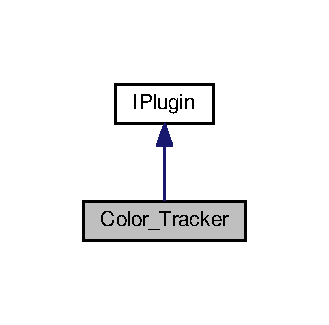
\includegraphics[width=158pt]{class_color___tracker__inherit__graph}
\end{center}
\end{figure}


Collaboration diagram for Color\+\_\+\+Tracker\+:\nopagebreak
\begin{figure}[H]
\begin{center}
\leavevmode
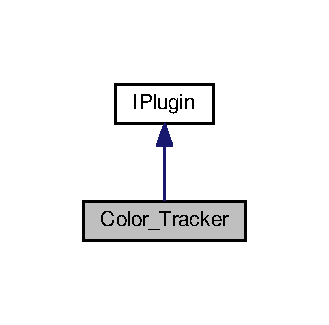
\includegraphics[width=158pt]{class_color___tracker__coll__graph}
\end{center}
\end{figure}
\subsection*{Public Member Functions}
\begin{DoxyCompactItemize}
\item 
void \hyperlink{class_color___tracker_a6d533ef7ecaea3ea1b2ae149f9336cec}{Main} ()
\begin{DoxyCompactList}\small\item\em Main funcction of the plugin. \end{DoxyCompactList}\item 
bool \hyperlink{class_color___tracker_a37bf24d89aac609cb6a773b86d4edcb6}{load\+Configuration} ()
\begin{DoxyCompactList}\small\item\em Load configuration. \end{DoxyCompactList}\item 
bool \hyperlink{class_color___tracker_a6382a354d9fa79f76c9586a195ea8674}{save\+Configuration} ()
\begin{DoxyCompactList}\small\item\em Save configuration. \end{DoxyCompactList}\item 
bool \hyperlink{class_color___tracker_a289707cab18e4af7f1353ee859da2fb5}{Initialize\+\_\+\+Output} ()
\begin{DoxyCompactList}\small\item\em Initialize Output variables for the plugin to publish. \end{DoxyCompactList}\item 
bool \hyperlink{class_color___tracker_afc447223ab3c357e66530b08acd8daea}{Initialize\+\_\+\+Input} ()
\begin{DoxyCompactList}\small\item\em Initialize Input variables for the plugin to publish. \end{DoxyCompactList}\item 
void \hyperlink{class_color___tracker_acc726eb03c58c22460c4f0440cfbc4cc}{stop} ()
\begin{DoxyCompactList}\small\item\em Stop plugin. \end{DoxyCompactList}\item 
void \hyperlink{class_color___tracker_a77d5ddbb266c0a13963fae15285ccc37}{run} ()
\begin{DoxyCompactList}\small\item\em Execute plugin. \end{DoxyCompactList}\end{DoxyCompactItemize}
\subsection*{Additional Inherited Members}


\subsection{Detailed Description}
\hyperlink{class_color___tracker}{Color\+\_\+\+Tracker} plugin. 

This plugin is an adaptation of Elias Ruiz color tracker for Gesture Therapy \begin{DoxyAuthor}{Author}
Patrick Heyer, \href{mailto:patrickhey@prodigy.net.mx}{\tt patrickhey@prodigy.\+net.\+mx} 
\end{DoxyAuthor}
\begin{DoxyDate}{Date}
jul 13, 2014 
\end{DoxyDate}
\begin{DoxyVersion}{Version}
1.\+0 
\end{DoxyVersion}


Definition at line 13 of file Color\+\_\+\+Tracker.\+h.



\subsection{Member Function Documentation}
\mbox{\Hypertarget{class_color___tracker_afc447223ab3c357e66530b08acd8daea}\label{class_color___tracker_afc447223ab3c357e66530b08acd8daea}} 
\index{Color\+\_\+\+Tracker@{Color\+\_\+\+Tracker}!Initialize\+\_\+\+Input@{Initialize\+\_\+\+Input}}
\index{Initialize\+\_\+\+Input@{Initialize\+\_\+\+Input}!Color\+\_\+\+Tracker@{Color\+\_\+\+Tracker}}
\subsubsection{\texorpdfstring{Initialize\+\_\+\+Input()}{Initialize\_Input()}}
{\footnotesize\ttfamily bool Color\+\_\+\+Tracker\+::\+Initialize\+\_\+\+Input (\begin{DoxyParamCaption}{ }\end{DoxyParamCaption})\hspace{0.3cm}{\ttfamily [virtual]}}



Initialize Input variables for the plugin to publish. 

\begin{DoxyReturn}{Returns}
bool 
\end{DoxyReturn}


Implements \hyperlink{class_i_plugin_aa7c66743ad956d8ada57becee559af4d}{I\+Plugin}.



Definition at line 156 of file Main.\+cpp.


\begin{DoxyCode}
157 \{
158     frame\_input = \textcolor{keyword}{static\_cast<}cv::Mat*\textcolor{keyword}{>}(Shared\_Memory::getInstance().Register\_Void\_Input(\textcolor{stringliteral}{"Video\_From\_Camera
      "}));
159     \textcolor{keywordflow}{return} \textcolor{keyword}{true};
160 \}
\end{DoxyCode}
\mbox{\Hypertarget{class_color___tracker_a289707cab18e4af7f1353ee859da2fb5}\label{class_color___tracker_a289707cab18e4af7f1353ee859da2fb5}} 
\index{Color\+\_\+\+Tracker@{Color\+\_\+\+Tracker}!Initialize\+\_\+\+Output@{Initialize\+\_\+\+Output}}
\index{Initialize\+\_\+\+Output@{Initialize\+\_\+\+Output}!Color\+\_\+\+Tracker@{Color\+\_\+\+Tracker}}
\subsubsection{\texorpdfstring{Initialize\+\_\+\+Output()}{Initialize\_Output()}}
{\footnotesize\ttfamily bool Color\+\_\+\+Tracker\+::\+Initialize\+\_\+\+Output (\begin{DoxyParamCaption}{ }\end{DoxyParamCaption})\hspace{0.3cm}{\ttfamily [virtual]}}



Initialize Output variables for the plugin to publish. 

\begin{DoxyReturn}{Returns}
bool 
\end{DoxyReturn}


Implements \hyperlink{class_i_plugin_a0b772513fc8c4ed01240e19c4bb84068}{I\+Plugin}.



Definition at line 151 of file Main.\+cpp.


\begin{DoxyCode}
152 \{
153     \textcolor{keywordflow}{return} \textcolor{keyword}{true};
154 \}
\end{DoxyCode}
\mbox{\Hypertarget{class_color___tracker_a37bf24d89aac609cb6a773b86d4edcb6}\label{class_color___tracker_a37bf24d89aac609cb6a773b86d4edcb6}} 
\index{Color\+\_\+\+Tracker@{Color\+\_\+\+Tracker}!load\+Configuration@{load\+Configuration}}
\index{load\+Configuration@{load\+Configuration}!Color\+\_\+\+Tracker@{Color\+\_\+\+Tracker}}
\subsubsection{\texorpdfstring{load\+Configuration()}{loadConfiguration()}}
{\footnotesize\ttfamily bool Color\+\_\+\+Tracker\+::load\+Configuration (\begin{DoxyParamCaption}{ }\end{DoxyParamCaption})\hspace{0.3cm}{\ttfamily [virtual]}}



Load configuration. 

The configuration can be loaded from file, or be hard coded into the plugin (not recomended), initialization of public and private variables should occur here

By default load\+Configuration is called during \hyperlink{class_plugin_manager_a956e653b7db36da9d034b4a93c8308d5}{Plugin\+Manager\+::\+Initialize()} by the plugin manager.

\begin{DoxyReturn}{Returns}
bool 
\end{DoxyReturn}


Implements \hyperlink{class_i_plugin_a418cff309436d3a15d9a4ce7369db6dd}{I\+Plugin}.



Definition at line 141 of file Main.\+cpp.


\begin{DoxyCode}
142 \{
143     \textcolor{keywordflow}{return} \textcolor{keyword}{true};
144 \}
\end{DoxyCode}
\mbox{\Hypertarget{class_color___tracker_a6d533ef7ecaea3ea1b2ae149f9336cec}\label{class_color___tracker_a6d533ef7ecaea3ea1b2ae149f9336cec}} 
\index{Color\+\_\+\+Tracker@{Color\+\_\+\+Tracker}!Main@{Main}}
\index{Main@{Main}!Color\+\_\+\+Tracker@{Color\+\_\+\+Tracker}}
\subsubsection{\texorpdfstring{Main()}{Main()}}
{\footnotesize\ttfamily void Color\+\_\+\+Tracker\+::\+Main (\begin{DoxyParamCaption}{ }\end{DoxyParamCaption})\hspace{0.3cm}{\ttfamily [virtual]}}



Main funcction of the plugin. 

Started in a new thread by the Run() funcction is the most importatn funcction of the plugin. Infinite loop (generaly a while(running) function that runs undefenitly in a read/process/write cicle). \begin{DoxyReturn}{Returns}
void 
\end{DoxyReturn}


Implements \hyperlink{class_i_plugin_ab5fdb3b0f7afdcee04324dca01766749}{I\+Plugin}.



Definition at line 60 of file Main.\+cpp.


\begin{DoxyCode}
61 \{
62     IplImage imgThresh;
63     \textcolor{keywordtype}{int} posX;
64     \textcolor{keywordtype}{int} posY;
65 
66     \textcolor{keywordflow}{while} (running)
67     \{
68         \textcolor{keywordflow}{if} (frame\_input->data != NULL)
69         \{
70             frame\_input->copyTo(frame);
71 
72 
73             cv::flip(frame, frame, 1);
74 
75 
76             cv::cvtColor(frame, HSV\_image, cv::COLOR\_BGR2HSV); \textcolor{comment}{//Convert the captured frame from BGR to HSV}
77             cv::inRange(HSV\_image, hsvlow, hsvhigh, HSV\_image); \textcolor{comment}{//Threshold the image}
78 
79             \textcolor{comment}{//morphological opening (removes small objects from the foreground)}
80             cv::erode(HSV\_image, HSV\_image, cv::getStructuringElement(cv::MORPH\_ELLIPSE, cv::Size(5, 5)));
81             cv::dilate(HSV\_image, HSV\_image, cv::getStructuringElement(cv::MORPH\_ELLIPSE, cv::Size(5, 5)));
82 
83             \textcolor{comment}{//morphological closing (removes small holes from the foreground)}
84             cv::dilate(HSV\_image, HSV\_image, cv::getStructuringElement(cv::MORPH\_ELLIPSE, cv::Size(5, 5)));
85             cv::erode(HSV\_image, HSV\_image, cv::getStructuringElement(cv::MORPH\_ELLIPSE, cv::Size(5, 5)));
86 
87             imgThresh = HSV\_image;
88             CvMoments *moments = (CvMoments*)malloc(\textcolor{keyword}{sizeof}(CvMoments));
89             cvMoments(&imgThresh, moments, 1);
90             \textcolor{keywordtype}{double} moment10 = cvGetSpatialMoment(moments, 1, 0);
91             \textcolor{keywordtype}{double} moment01 = cvGetSpatialMoment(moments, 0, 1);
92             \textcolor{keywordtype}{double} area = cvGetCentralMoment(moments, 0, 0);
93             cv::RNG rng(12345);
94             cv::Scalar color = cv::Scalar(rng.uniform(0, 255), rng.uniform(0, 255), rng.uniform(0, 255));
95             \textcolor{comment}{// if the area<1000, I consider that the there are no object in the image and it's because of
       the noise, the area is not zero}
96 
97 
98             cv::Point center;
99             center.x = posX;
100             center.y = posY;
101 
102             cv::circle(frame,center, sqrt(area*.5), color, 2, 8, 0);
103 
104 
105             free(moments);
106 
107             \textcolor{comment}{//cv::imshow("Thresholded Image", HSV\_image); //show the thresholded image}
108             cv::imshow(\textcolor{stringliteral}{"edges"}, frame);
109 
110             cv::setMouseCallback(\textcolor{stringliteral}{"edges"}, getHSV, 0);
111             
112 
113         \}
114         cv::waitKey(10);
115         
116     \}
117    
118 
119     stoped = \textcolor{keyword}{true};
120     \textcolor{keywordflow}{return};
121 \}
\end{DoxyCode}
\mbox{\Hypertarget{class_color___tracker_a77d5ddbb266c0a13963fae15285ccc37}\label{class_color___tracker_a77d5ddbb266c0a13963fae15285ccc37}} 
\index{Color\+\_\+\+Tracker@{Color\+\_\+\+Tracker}!run@{run}}
\index{run@{run}!Color\+\_\+\+Tracker@{Color\+\_\+\+Tracker}}
\subsubsection{\texorpdfstring{run()}{run()}}
{\footnotesize\ttfamily void Color\+\_\+\+Tracker\+::run (\begin{DoxyParamCaption}{ }\end{DoxyParamCaption})\hspace{0.3cm}{\ttfamily [virtual]}}



Execute plugin. 

Starts a new thread and executes the plugins main() funcction. \begin{DoxyReturn}{Returns}
void 
\end{DoxyReturn}


Implements \hyperlink{class_i_plugin_a46b4ace767e77f9db9c9585e99c09039}{I\+Plugin}.



Definition at line 161 of file Main.\+cpp.



References I\+Plugin\+::\+Inc\+Wrapper().


\begin{DoxyCode}
162 \{
163     pthread\_create(&thread\_id, NULL, &\hyperlink{class_i_plugin_a62d22be2fdf66eb7f5c2f797f5f3d7f3}{IPlugin::IncWrapper}, \textcolor{keyword}{this});
164     running = \textcolor{keyword}{true};
165     stoped = \textcolor{keyword}{false};
166 \}
\end{DoxyCode}
\mbox{\Hypertarget{class_color___tracker_a6382a354d9fa79f76c9586a195ea8674}\label{class_color___tracker_a6382a354d9fa79f76c9586a195ea8674}} 
\index{Color\+\_\+\+Tracker@{Color\+\_\+\+Tracker}!save\+Configuration@{save\+Configuration}}
\index{save\+Configuration@{save\+Configuration}!Color\+\_\+\+Tracker@{Color\+\_\+\+Tracker}}
\subsubsection{\texorpdfstring{save\+Configuration()}{saveConfiguration()}}
{\footnotesize\ttfamily bool Color\+\_\+\+Tracker\+::save\+Configuration (\begin{DoxyParamCaption}{ }\end{DoxyParamCaption})\hspace{0.3cm}{\ttfamily [virtual]}}



Save configuration. 

The configuration should be saved to file, public and private variables that should be configured at startup should be saved.

By default save\+Configuration is called during \hyperlink{class_plugin_manager_ab651a05d6fcb92562807e9f5ecc30855}{Plugin\+Manager\+::\+Unload()} by the plugin manager.

\begin{DoxyReturn}{Returns}
bool 
\end{DoxyReturn}


Implements \hyperlink{class_i_plugin_a79b5c42b1c7b08257a6110b2091039bc}{I\+Plugin}.



Definition at line 146 of file Main.\+cpp.


\begin{DoxyCode}
147 \{
148     \textcolor{keywordflow}{return} \textcolor{keyword}{true};
149 \}
\end{DoxyCode}
\mbox{\Hypertarget{class_color___tracker_acc726eb03c58c22460c4f0440cfbc4cc}\label{class_color___tracker_acc726eb03c58c22460c4f0440cfbc4cc}} 
\index{Color\+\_\+\+Tracker@{Color\+\_\+\+Tracker}!stop@{stop}}
\index{stop@{stop}!Color\+\_\+\+Tracker@{Color\+\_\+\+Tracker}}
\subsubsection{\texorpdfstring{stop()}{stop()}}
{\footnotesize\ttfamily void Color\+\_\+\+Tracker\+::stop (\begin{DoxyParamCaption}{ }\end{DoxyParamCaption})\hspace{0.3cm}{\ttfamily [virtual]}}



Stop plugin. 

Stops the plugin \begin{DoxyReturn}{Returns}
void 
\end{DoxyReturn}


Implements \hyperlink{class_i_plugin_a86e523c283aec5c9fb21249a76e916ac}{I\+Plugin}.



Definition at line 168 of file Main.\+cpp.


\begin{DoxyCode}
169 \{
170     running = \textcolor{keyword}{false};
171 
172 \}
\end{DoxyCode}


The documentation for this class was generated from the following files\+:\begin{DoxyCompactItemize}
\item 
/home/patrick/projects/\+Gesture\+\_\+\+Therapy\+\_\+\+Linux/src/\+Color\+\_\+\+Tracker/Color\+\_\+\+Tracker.\+h\item 
/home/patrick/projects/\+Gesture\+\_\+\+Therapy\+\_\+\+Linux/src/\+Color\+\_\+\+Tracker/Main.\+cpp\end{DoxyCompactItemize}

\hypertarget{class_config_file}{}\section{Config\+File Class Reference}
\label{class_config_file}\index{Config\+File@{Config\+File}}


Collaboration diagram for Config\+File\+:\nopagebreak
\begin{figure}[H]
\begin{center}
\leavevmode
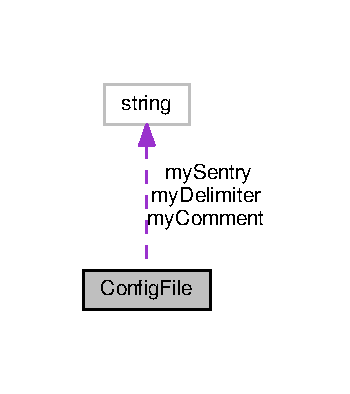
\includegraphics[width=168pt]{class_config_file__coll__graph}
\end{center}
\end{figure}
\subsection*{Classes}
\begin{DoxyCompactItemize}
\item 
struct \hyperlink{struct_config_file_1_1file__not__found}{file\+\_\+not\+\_\+found}
\item 
struct \hyperlink{struct_config_file_1_1key__not__found}{key\+\_\+not\+\_\+found}
\end{DoxyCompactItemize}
\subsection*{Public Member Functions}
\begin{DoxyCompactItemize}
\item 
\mbox{\Hypertarget{class_config_file_a2690c3c6b72869b65d168791b28264dc}\label{class_config_file_a2690c3c6b72869b65d168791b28264dc}} 
{\bfseries Config\+File} (string filename, string delimiter=\char`\"{}=\char`\"{}, string comment=\char`\"{}\#\char`\"{}, string sentry=\char`\"{}End\+Config\+File\char`\"{})
\item 
\mbox{\Hypertarget{class_config_file_af6ac80a51f87386592c346c02e7e4e50}\label{class_config_file_af6ac80a51f87386592c346c02e7e4e50}} 
{\footnotesize template$<$class T $>$ }\\T {\bfseries read} (const string \&key) const
\item 
\mbox{\Hypertarget{class_config_file_a44eba9d0ac0ec6a05bf35705a2f9dfe4}\label{class_config_file_a44eba9d0ac0ec6a05bf35705a2f9dfe4}} 
{\footnotesize template$<$class T $>$ }\\T {\bfseries read} (const string \&key, const T \&value) const
\item 
\mbox{\Hypertarget{class_config_file_a13d3da6885ae145204afff039d190a75}\label{class_config_file_a13d3da6885ae145204afff039d190a75}} 
{\footnotesize template$<$class T $>$ }\\bool {\bfseries read\+Into} (T \&var, const string \&key) const
\item 
\mbox{\Hypertarget{class_config_file_a43b40ec4b9933a2bb57655f21763d4d4}\label{class_config_file_a43b40ec4b9933a2bb57655f21763d4d4}} 
{\footnotesize template$<$class T $>$ }\\bool {\bfseries read\+Into} (T \&var, const string \&key, const T \&value) const
\item 
\mbox{\Hypertarget{class_config_file_ad82a9c27d698a5e805cf5f6f0ad1bfd5}\label{class_config_file_ad82a9c27d698a5e805cf5f6f0ad1bfd5}} 
{\footnotesize template$<$class T $>$ }\\void {\bfseries add} (string key, const T \&value)
\item 
\mbox{\Hypertarget{class_config_file_afca295f72101b138ad2702a11c342f37}\label{class_config_file_afca295f72101b138ad2702a11c342f37}} 
void {\bfseries remove} (const string \&key)
\item 
\mbox{\Hypertarget{class_config_file_a9cb492eb48dad9f2edd14b3799e5e10e}\label{class_config_file_a9cb492eb48dad9f2edd14b3799e5e10e}} 
bool {\bfseries key\+Exists} (const string \&key) const
\item 
\mbox{\Hypertarget{class_config_file_ad5c780c8af0dc1c7cc701d1bbfe39dc2}\label{class_config_file_ad5c780c8af0dc1c7cc701d1bbfe39dc2}} 
string {\bfseries get\+Delimiter} () const
\item 
\mbox{\Hypertarget{class_config_file_a37b222022f77e1837b773a2e8ebed519}\label{class_config_file_a37b222022f77e1837b773a2e8ebed519}} 
string {\bfseries get\+Comment} () const
\item 
\mbox{\Hypertarget{class_config_file_a41cd2b14758fd3c647b4591cd7ded327}\label{class_config_file_a41cd2b14758fd3c647b4591cd7ded327}} 
string {\bfseries get\+Sentry} () const
\item 
\mbox{\Hypertarget{class_config_file_af28390aba7d8f399ac734c074e659b99}\label{class_config_file_af28390aba7d8f399ac734c074e659b99}} 
string {\bfseries set\+Delimiter} (const string \&s)
\item 
\mbox{\Hypertarget{class_config_file_a2e06b3000fb45426c975b334b2cee148}\label{class_config_file_a2e06b3000fb45426c975b334b2cee148}} 
string {\bfseries set\+Comment} (const string \&s)
\end{DoxyCompactItemize}
\subsection*{Protected Types}
\begin{DoxyCompactItemize}
\item 
\mbox{\Hypertarget{class_config_file_a91de4778982f558673be7465f33750f5}\label{class_config_file_a91de4778982f558673be7465f33750f5}} 
typedef std\+::map$<$ string, string $>$\+::iterator {\bfseries mapi}
\item 
\mbox{\Hypertarget{class_config_file_af606aa032e366450b81792da67c984fc}\label{class_config_file_af606aa032e366450b81792da67c984fc}} 
typedef std\+::map$<$ string, string $>$\+::const\+\_\+iterator {\bfseries mapci}
\end{DoxyCompactItemize}
\subsection*{Protected Member Functions}
\begin{DoxyCompactItemize}
\item 
\mbox{\Hypertarget{class_config_file_a7d2b8acc0f7c2ea7892ef2e77d925ba9}\label{class_config_file_a7d2b8acc0f7c2ea7892ef2e77d925ba9}} 
{\footnotesize template$<$$>$ }\\string {\bfseries string\+\_\+as\+\_\+T} (const string \&s)
\item 
\mbox{\Hypertarget{class_config_file_adda9a4a7de5eef0151e45b5874ddf50d}\label{class_config_file_adda9a4a7de5eef0151e45b5874ddf50d}} 
{\footnotesize template$<$$>$ }\\bool {\bfseries string\+\_\+as\+\_\+T} (const string \&s)
\end{DoxyCompactItemize}
\subsection*{Static Protected Member Functions}
\begin{DoxyCompactItemize}
\item 
\mbox{\Hypertarget{class_config_file_a9855bff7ed5af9aa408ac06fc7ab4c09}\label{class_config_file_a9855bff7ed5af9aa408ac06fc7ab4c09}} 
{\footnotesize template$<$class T $>$ }\\static string {\bfseries T\+\_\+as\+\_\+string} (const T \&t)
\item 
\mbox{\Hypertarget{class_config_file_a59c6ab56cdfa23a29a38bf3eea1ededf}\label{class_config_file_a59c6ab56cdfa23a29a38bf3eea1ededf}} 
{\footnotesize template$<$class T $>$ }\\static T {\bfseries string\+\_\+as\+\_\+T} (const string \&s)
\item 
\mbox{\Hypertarget{class_config_file_a6b445b393fcf42386a804fc4077fac10}\label{class_config_file_a6b445b393fcf42386a804fc4077fac10}} 
static void {\bfseries trim} (string \&s)
\end{DoxyCompactItemize}
\subsection*{Protected Attributes}
\begin{DoxyCompactItemize}
\item 
\mbox{\Hypertarget{class_config_file_ad63f3e259f665192b64fb3e83c701425}\label{class_config_file_ad63f3e259f665192b64fb3e83c701425}} 
string {\bfseries my\+Delimiter}
\item 
\mbox{\Hypertarget{class_config_file_a2c60a141e8ad012b86a0642ec8ec638d}\label{class_config_file_a2c60a141e8ad012b86a0642ec8ec638d}} 
string {\bfseries my\+Comment}
\item 
\mbox{\Hypertarget{class_config_file_af066ec1942c50848a055350029ebbca5}\label{class_config_file_af066ec1942c50848a055350029ebbca5}} 
string {\bfseries my\+Sentry}
\item 
\mbox{\Hypertarget{class_config_file_a91b9b9e241d42bd3b1bb8b3e6355761f}\label{class_config_file_a91b9b9e241d42bd3b1bb8b3e6355761f}} 
std\+::map$<$ string, string $>$ {\bfseries my\+Contents}
\end{DoxyCompactItemize}
\subsection*{Friends}
\begin{DoxyCompactItemize}
\item 
\mbox{\Hypertarget{class_config_file_a8ccacbc37db1992a5515e2c72fc83ce6}\label{class_config_file_a8ccacbc37db1992a5515e2c72fc83ce6}} 
std\+::ostream \& {\bfseries operator$<$$<$} (std\+::ostream \&os, const \hyperlink{class_config_file}{Config\+File} \&cf)
\item 
\mbox{\Hypertarget{class_config_file_a25042475439039e70f90febe7d0e63ec}\label{class_config_file_a25042475439039e70f90febe7d0e63ec}} 
std\+::istream \& {\bfseries operator$>$$>$} (std\+::istream \&is, \hyperlink{class_config_file}{Config\+File} \&cf)
\end{DoxyCompactItemize}


\subsection{Detailed Description}


Definition at line 54 of file Config\+File.\+h.



The documentation for this class was generated from the following files\+:\begin{DoxyCompactItemize}
\item 
/home/patrick/projects/\+Gesture\+\_\+\+Therapy\+\_\+\+Linux/src/include/Config\+File.\+h\item 
/home/patrick/projects/\+Gesture\+\_\+\+Therapy\+\_\+\+Linux/src/include/Config\+File.\+cpp\end{DoxyCompactItemize}

\hypertarget{struct_config_file_1_1file__not__found}{}\section{Config\+File\+:\+:file\+\_\+not\+\_\+found Struct Reference}
\label{struct_config_file_1_1file__not__found}\index{Config\+File\+::file\+\_\+not\+\_\+found@{Config\+File\+::file\+\_\+not\+\_\+found}}


Collaboration diagram for Config\+File\+:\+:file\+\_\+not\+\_\+found\+:\nopagebreak
\begin{figure}[H]
\begin{center}
\leavevmode
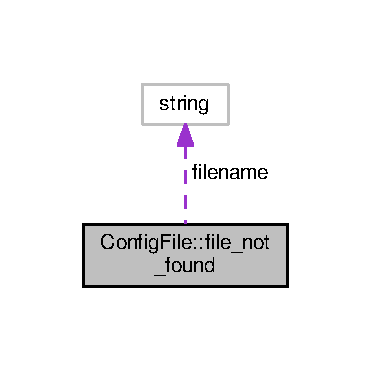
\includegraphics[width=178pt]{struct_config_file_1_1file__not__found__coll__graph}
\end{center}
\end{figure}
\subsection*{Public Member Functions}
\begin{DoxyCompactItemize}
\item 
\mbox{\Hypertarget{struct_config_file_1_1file__not__found_ab0fa2b6e7d1891136f82d4baf124725b}\label{struct_config_file_1_1file__not__found_ab0fa2b6e7d1891136f82d4baf124725b}} 
{\bfseries file\+\_\+not\+\_\+found} (const string \&filename\+\_\+=string())
\end{DoxyCompactItemize}
\subsection*{Public Attributes}
\begin{DoxyCompactItemize}
\item 
\mbox{\Hypertarget{struct_config_file_1_1file__not__found_a25e11d11b1a9b0f4ca663b21816c2a9a}\label{struct_config_file_1_1file__not__found_a25e11d11b1a9b0f4ca663b21816c2a9a}} 
string {\bfseries filename}
\end{DoxyCompactItemize}


\subsection{Detailed Description}


Definition at line 108 of file Config\+File.\+h.



The documentation for this struct was generated from the following file\+:\begin{DoxyCompactItemize}
\item 
/home/patrick/projects/\+Gesture\+\_\+\+Therapy\+\_\+\+Linux/src/include/Config\+File.\+h\end{DoxyCompactItemize}

\hypertarget{class_file___writer}{}\section{File\+\_\+\+Writer Class Reference}
\label{class_file___writer}\index{File\+\_\+\+Writer@{File\+\_\+\+Writer}}


\hyperlink{class_file___writer}{File\+\_\+\+Writer} plugin.  




{\ttfamily \#include $<$File\+\_\+\+Writer.\+h$>$}



Inheritance diagram for File\+\_\+\+Writer\+:\nopagebreak
\begin{figure}[H]
\begin{center}
\leavevmode
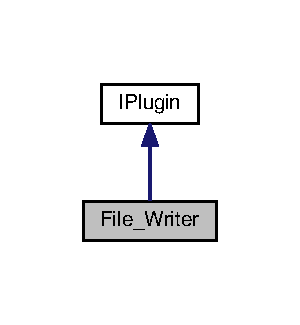
\includegraphics[width=144pt]{class_file___writer__inherit__graph}
\end{center}
\end{figure}


Collaboration diagram for File\+\_\+\+Writer\+:\nopagebreak
\begin{figure}[H]
\begin{center}
\leavevmode
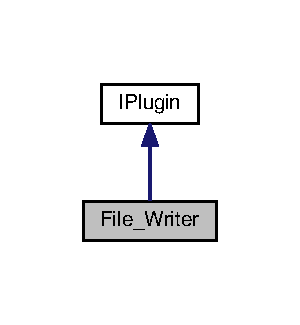
\includegraphics[width=144pt]{class_file___writer__coll__graph}
\end{center}
\end{figure}
\subsection*{Public Member Functions}
\begin{DoxyCompactItemize}
\item 
void \hyperlink{class_file___writer_a0738556056b69f64bf524fee06a6e69f}{Main} ()
\begin{DoxyCompactList}\small\item\em Main funcction of the plugin. \end{DoxyCompactList}\item 
bool \hyperlink{class_file___writer_a8f9010f501d8349bd9e8895405a8de8b}{load\+Configuration} ()
\begin{DoxyCompactList}\small\item\em Load configuration. \end{DoxyCompactList}\item 
bool \hyperlink{class_file___writer_a6561b234c4ce33315aa5931463a1cb20}{save\+Configuration} ()
\begin{DoxyCompactList}\small\item\em Save configuration. \end{DoxyCompactList}\item 
bool \hyperlink{class_file___writer_a7450494cfffa8ba1635f9121dfd955de}{Initialize\+\_\+\+Output} ()
\begin{DoxyCompactList}\small\item\em Initialize Output variables for the plugin to publish. \end{DoxyCompactList}\item 
bool \hyperlink{class_file___writer_a13697d8b3249804553ef61a54fea5ce1}{Initialize\+\_\+\+Input} ()
\begin{DoxyCompactList}\small\item\em Initialize Input variables for the plugin to publish. \end{DoxyCompactList}\item 
void \hyperlink{class_file___writer_a3a7de57b86f801257806115b54136fd7}{run} ()
\begin{DoxyCompactList}\small\item\em Execute plugin. \end{DoxyCompactList}\item 
void \hyperlink{class_file___writer_ad420a007be3af0efd8ea76bac66e2cb0}{stop} ()
\begin{DoxyCompactList}\small\item\em Stop plugin. \end{DoxyCompactList}\end{DoxyCompactItemize}
\subsection*{Additional Inherited Members}


\subsection{Detailed Description}
\hyperlink{class_file___writer}{File\+\_\+\+Writer} plugin. 

This plugin is a network server that accepts client conections to comunicate with other programs (running on the same computer or over the network) \begin{DoxyAuthor}{Author}
Patrick Heyer, \href{mailto:patrickhey@prodigy.net.mx}{\tt patrickhey@prodigy.\+net.\+mx}, Juan Herrera \href{mailto:juan_antonio_@hotmail.com}{\tt juan\+\_\+antonio\+\_\+@hotmail.\+com}, Manuel Oropeza \href{mailto:zodiacanimations@msn.com}{\tt zodiacanimations@msn.\+com} 
\end{DoxyAuthor}
\begin{DoxyDate}{Date}
jul 04, 2012 
\end{DoxyDate}
\begin{DoxyVersion}{Version}
1.\+0 
\end{DoxyVersion}


Definition at line 13 of file File\+\_\+\+Writer.\+h.



\subsection{Member Function Documentation}
\mbox{\Hypertarget{class_file___writer_a13697d8b3249804553ef61a54fea5ce1}\label{class_file___writer_a13697d8b3249804553ef61a54fea5ce1}} 
\index{File\+\_\+\+Writer@{File\+\_\+\+Writer}!Initialize\+\_\+\+Input@{Initialize\+\_\+\+Input}}
\index{Initialize\+\_\+\+Input@{Initialize\+\_\+\+Input}!File\+\_\+\+Writer@{File\+\_\+\+Writer}}
\subsubsection{\texorpdfstring{Initialize\+\_\+\+Input()}{Initialize\_Input()}}
{\footnotesize\ttfamily bool File\+\_\+\+Writer\+::\+Initialize\+\_\+\+Input (\begin{DoxyParamCaption}{ }\end{DoxyParamCaption})\hspace{0.3cm}{\ttfamily [virtual]}}



Initialize Input variables for the plugin to publish. 

\begin{DoxyReturn}{Returns}
bool 
\end{DoxyReturn}


Implements \hyperlink{class_i_plugin_aa7c66743ad956d8ada57becee559af4d}{I\+Plugin}.



Definition at line 150 of file Main.\+cpp.


\begin{DoxyCode}
151 \{
152 
153     RShoulder\_X=Shared\_Memory::getInstance().Register\_Double\_Input(\textcolor{stringliteral}{"RIGHT\_SHOULDER\_X"});
154     RShoulder\_Y=Shared\_Memory::getInstance().Register\_Double\_Input(\textcolor{stringliteral}{"RIGHT\_SHOULDER\_Y"});
155     RShoulder\_Z=Shared\_Memory::getInstance().Register\_Double\_Input(\textcolor{stringliteral}{"RIGHT\_SHOULDER\_Z"});
156     RElbow\_X=Shared\_Memory::getInstance().Register\_Double\_Input(\textcolor{stringliteral}{"RIGHT\_ELBOW\_X"});
157     RElbow\_Y=Shared\_Memory::getInstance().Register\_Double\_Input(\textcolor{stringliteral}{"RIGHT\_ELBOW\_Y"});
158     RElbow\_Z=Shared\_Memory::getInstance().Register\_Double\_Input(\textcolor{stringliteral}{"RIGHT\_ELBOW\_Z"});
159     RHand\_X=Shared\_Memory::getInstance().Register\_Double\_Input(\textcolor{stringliteral}{"RIGHT\_HAND\_X"});
160     RHand\_Y=Shared\_Memory::getInstance().Register\_Double\_Input(\textcolor{stringliteral}{"RIGHT\_HAND\_Y"});
161     RHand\_Z=Shared\_Memory::getInstance().Register\_Double\_Input(\textcolor{stringliteral}{"RIGHT\_HAND\_Z"});
162 
163     LShoulder\_X=Shared\_Memory::getInstance().Register\_Double\_Input(\textcolor{stringliteral}{"LEFT\_SHOULDER\_X"});
164     LShoulder\_Y=Shared\_Memory::getInstance().Register\_Double\_Input(\textcolor{stringliteral}{"LEFT\_SHOULDER\_Y"});
165     LShoulder\_Z=Shared\_Memory::getInstance().Register\_Double\_Input(\textcolor{stringliteral}{"LEFT\_SHOULDER\_Z"});
166     LElbow\_X=Shared\_Memory::getInstance().Register\_Double\_Input(\textcolor{stringliteral}{"LEFT\_ELBOW\_X"});
167     LElbow\_Y=Shared\_Memory::getInstance().Register\_Double\_Input(\textcolor{stringliteral}{"LEFT\_ELBOW\_Y"});
168     LElbow\_Z=Shared\_Memory::getInstance().Register\_Double\_Input(\textcolor{stringliteral}{"LEFT\_ELBOW\_Z"});
169     LHand\_X=Shared\_Memory::getInstance().Register\_Double\_Input(\textcolor{stringliteral}{"LEFT\_HAND\_X"});
170     LHand\_Y=Shared\_Memory::getInstance().Register\_Double\_Input(\textcolor{stringliteral}{"LEFT\_HAND\_Y"});
171     LHand\_Z=Shared\_Memory::getInstance().Register\_Double\_Input(\textcolor{stringliteral}{"LEFT\_HAND\_Z"});
172 
173     Torso\_X=Shared\_Memory::getInstance().Register\_Double\_Input(\textcolor{stringliteral}{"TORSO\_X"});
174     Torso\_Y=Shared\_Memory::getInstance().Register\_Double\_Input(\textcolor{stringliteral}{"TORSO\_Y"});
175     Torso\_Z=Shared\_Memory::getInstance().Register\_Double\_Input(\textcolor{stringliteral}{"TORSO\_Z"});
176 
177     Head\_X=Shared\_Memory::getInstance().Register\_Double\_Input(\textcolor{stringliteral}{"HEAD\_X"});
178     Head\_Y=Shared\_Memory::getInstance().Register\_Double\_Input(\textcolor{stringliteral}{"HEAD\_Y"});
179     Head\_Z=Shared\_Memory::getInstance().Register\_Double\_Input(\textcolor{stringliteral}{"HEAD\_Z"});
180 \textcolor{comment}{/*}
181 \textcolor{comment}{    BTGripper\_X=Shared\_Memory::getInstance().Register\_Double\_Input("BTGripper\_X");
}
182 \textcolor{comment}{    BTGripper\_Y=Shared\_Memory::getInstance().Register\_Double\_Input("BTGripper\_Y");
}
183 \textcolor{comment}{    BTGripper\_Z=Shared\_Memory::getInstance().Register\_Double\_Input("BTGripper\_Z");*/}
184 
185     LPMS\_QUAT\_W=Shared\_Memory::getInstance().Register\_Double\_Input(\textcolor{stringliteral}{"LPMS\_QUAT\_W"});
186     LPMS\_QUAT\_X=Shared\_Memory::getInstance().Register\_Double\_Input(\textcolor{stringliteral}{"LPMS\_QUAT\_X"});
187     LPMS\_QUAT\_Y=Shared\_Memory::getInstance().Register\_Double\_Input(\textcolor{stringliteral}{"LPMS\_QUAT\_Y"});
188     LPMS\_QUAT\_Z=Shared\_Memory::getInstance().Register\_Double\_Input(\textcolor{stringliteral}{"LPMS\_QUAT\_Z"});
189 
190 
191     LPMS\_QUAT\_W=Shared\_Memory::getInstance().Register\_Double\_Input(\textcolor{stringliteral}{"LPMS\_QUAT\_W"});
192     LPMS\_QUAT\_X=Shared\_Memory::getInstance().Register\_Double\_Input(\textcolor{stringliteral}{"LPMS\_QUAT\_X"});
193     LPMS\_QUAT\_Y=Shared\_Memory::getInstance().Register\_Double\_Input(\textcolor{stringliteral}{"LPMS\_QUAT\_Y"});
194     LPMS\_QUAT\_Z=Shared\_Memory::getInstance().Register\_Double\_Input(\textcolor{stringliteral}{"LPMS\_QUAT\_Z"});
195 
196     LPMS\_ACCEL\_RAW\_X=Shared\_Memory::getInstance().Register\_Double\_Input(\textcolor{stringliteral}{"LPMS\_ACCEL\_RAW\_X"});
197     LPMS\_ACCEL\_RAW\_Y=Shared\_Memory::getInstance().Register\_Double\_Input(\textcolor{stringliteral}{"LPMS\_ACCEL\_RAW\_Y"});
198     LPMS\_ACCEL\_RAW\_Z=Shared\_Memory::getInstance().Register\_Double\_Input(\textcolor{stringliteral}{"LPMS\_ACCEL\_RAW\_Z"});
199 
200     LPMS\_GYRO\_RAW\_X=Shared\_Memory::getInstance().Register\_Double\_Input(\textcolor{stringliteral}{"LPMS\_GYRO\_RAW\_X"});
201     LPMS\_GYRO\_RAW\_Y=Shared\_Memory::getInstance().Register\_Double\_Input(\textcolor{stringliteral}{"LPMS\_GYRO\_RAW\_Y"});
202     LPMS\_GYRO\_RAW\_Z=Shared\_Memory::getInstance().Register\_Double\_Input(\textcolor{stringliteral}{"LPMS\_GYRO\_RAW\_Z"});
203 
204     LPMS\_MAT\_11=Shared\_Memory::getInstance().Register\_Double\_Input(\textcolor{stringliteral}{"LPMS\_MAT\_11"});
205     LPMS\_MAT\_12=Shared\_Memory::getInstance().Register\_Double\_Input(\textcolor{stringliteral}{"LPMS\_MAT\_12"});
206     LPMS\_MAT\_13=Shared\_Memory::getInstance().Register\_Double\_Input(\textcolor{stringliteral}{"LPMS\_MAT\_13"});
207     LPMS\_MAT\_21=Shared\_Memory::getInstance().Register\_Double\_Input(\textcolor{stringliteral}{"LPMS\_MAT\_21"});
208     LPMS\_MAT\_22=Shared\_Memory::getInstance().Register\_Double\_Input(\textcolor{stringliteral}{"LPMS\_MAT\_22"});
209     LPMS\_MAT\_23=Shared\_Memory::getInstance().Register\_Double\_Input(\textcolor{stringliteral}{"LPMS\_MAT\_23"});
210     LPMS\_MAT\_31=Shared\_Memory::getInstance().Register\_Double\_Input(\textcolor{stringliteral}{"LPMS\_MAT\_31"});
211     LPMS\_MAT\_32=Shared\_Memory::getInstance().Register\_Double\_Input(\textcolor{stringliteral}{"LPMS\_MAT\_32"});
212     LPMS\_MAT\_33=Shared\_Memory::getInstance().Register\_Double\_Input(\textcolor{stringliteral}{"LPMS\_MAT\_33"});
213 
214     LPMS\_MAT\_OFFSET\_11=Shared\_Memory::getInstance().Register\_Double\_Input(\textcolor{stringliteral}{"LPMS\_MAT\_OFFSET\_11"});
215     LPMS\_MAT\_OFFSET\_12=Shared\_Memory::getInstance().Register\_Double\_Input(\textcolor{stringliteral}{"LPMS\_MAT\_OFFSET\_12"});
216     LPMS\_MAT\_OFFSET\_13=Shared\_Memory::getInstance().Register\_Double\_Input(\textcolor{stringliteral}{"LPMS\_MAT\_OFFSET\_13"});
217     LPMS\_MAT\_OFFSET\_21=Shared\_Memory::getInstance().Register\_Double\_Input(\textcolor{stringliteral}{"LPMS\_MAT\_OFFSET\_21"});
218     LPMS\_MAT\_OFFSET\_22=Shared\_Memory::getInstance().Register\_Double\_Input(\textcolor{stringliteral}{"LPMS\_MAT\_OFFSET\_22"});
219     LPMS\_MAT\_OFFSET\_23=Shared\_Memory::getInstance().Register\_Double\_Input(\textcolor{stringliteral}{"LPMS\_MAT\_OFFSET\_23"});
220     LPMS\_MAT\_OFFSET\_31=Shared\_Memory::getInstance().Register\_Double\_Input(\textcolor{stringliteral}{"LPMS\_MAT\_OFFSET\_31"});
221     LPMS\_MAT\_OFFSET\_32=Shared\_Memory::getInstance().Register\_Double\_Input(\textcolor{stringliteral}{"LPMS\_MAT\_OFFSET\_32"});
222     LPMS\_MAT\_OFFSET\_33=Shared\_Memory::getInstance().Register\_Double\_Input(\textcolor{stringliteral}{"LPMS\_MAT\_OFFSET\_33"});
223 
224     \textcolor{keywordflow}{return} \textcolor{keyword}{true};
225 \}
\end{DoxyCode}
\mbox{\Hypertarget{class_file___writer_a7450494cfffa8ba1635f9121dfd955de}\label{class_file___writer_a7450494cfffa8ba1635f9121dfd955de}} 
\index{File\+\_\+\+Writer@{File\+\_\+\+Writer}!Initialize\+\_\+\+Output@{Initialize\+\_\+\+Output}}
\index{Initialize\+\_\+\+Output@{Initialize\+\_\+\+Output}!File\+\_\+\+Writer@{File\+\_\+\+Writer}}
\subsubsection{\texorpdfstring{Initialize\+\_\+\+Output()}{Initialize\_Output()}}
{\footnotesize\ttfamily bool File\+\_\+\+Writer\+::\+Initialize\+\_\+\+Output (\begin{DoxyParamCaption}{ }\end{DoxyParamCaption})\hspace{0.3cm}{\ttfamily [virtual]}}



Initialize Output variables for the plugin to publish. 

\begin{DoxyReturn}{Returns}
bool 
\end{DoxyReturn}


Implements \hyperlink{class_i_plugin_a0b772513fc8c4ed01240e19c4bb84068}{I\+Plugin}.



Definition at line 145 of file Main.\+cpp.


\begin{DoxyCode}
146 \{
147     \textcolor{keywordflow}{return} \textcolor{keyword}{true};
148 \}
\end{DoxyCode}
\mbox{\Hypertarget{class_file___writer_a8f9010f501d8349bd9e8895405a8de8b}\label{class_file___writer_a8f9010f501d8349bd9e8895405a8de8b}} 
\index{File\+\_\+\+Writer@{File\+\_\+\+Writer}!load\+Configuration@{load\+Configuration}}
\index{load\+Configuration@{load\+Configuration}!File\+\_\+\+Writer@{File\+\_\+\+Writer}}
\subsubsection{\texorpdfstring{load\+Configuration()}{loadConfiguration()}}
{\footnotesize\ttfamily bool File\+\_\+\+Writer\+::load\+Configuration (\begin{DoxyParamCaption}{ }\end{DoxyParamCaption})\hspace{0.3cm}{\ttfamily [virtual]}}



Load configuration. 

The configuration can be loaded from file, or be hard coded into the plugin (not recomended), initialization of public and private variables should occur here

By default load\+Configuration is called during \hyperlink{class_plugin_manager_a956e653b7db36da9d034b4a93c8308d5}{Plugin\+Manager\+::\+Initialize()} by the plugin manager.

\begin{DoxyReturn}{Returns}
bool 
\end{DoxyReturn}


Implements \hyperlink{class_i_plugin_a418cff309436d3a15d9a4ce7369db6dd}{I\+Plugin}.



Definition at line 126 of file Main.\+cpp.


\begin{DoxyCode}
127 \{
128     std::stringstream path;
129     path <<\textcolor{stringliteral}{"../conf/"} << PLUGIN\_NAME;
130     \hyperlink{class_config_file}{ConfigFile} config( path.str() );
131     \textcolor{keywordflow}{return} \textcolor{keyword}{true};
132 \}
\end{DoxyCode}
\mbox{\Hypertarget{class_file___writer_a0738556056b69f64bf524fee06a6e69f}\label{class_file___writer_a0738556056b69f64bf524fee06a6e69f}} 
\index{File\+\_\+\+Writer@{File\+\_\+\+Writer}!Main@{Main}}
\index{Main@{Main}!File\+\_\+\+Writer@{File\+\_\+\+Writer}}
\subsubsection{\texorpdfstring{Main()}{Main()}}
{\footnotesize\ttfamily void File\+\_\+\+Writer\+::\+Main (\begin{DoxyParamCaption}{ }\end{DoxyParamCaption})\hspace{0.3cm}{\ttfamily [virtual]}}



Main funcction of the plugin. 

Started in a new thread by the Run() funcction is the most importatn funcction of the plugin. Infinite loop (generaly a while(running) function that runs undefenitly in a read/process/write cicle). \begin{DoxyReturn}{Returns}
void 
\end{DoxyReturn}


Implements \hyperlink{class_i_plugin_ab5fdb3b0f7afdcee04324dca01766749}{I\+Plugin}.



Definition at line 49 of file Main.\+cpp.



References save\+Configuration().


\begin{DoxyCode}
50 \{
51 \textcolor{preprocessor}{    #ifdef OPENGL\_GUI
}
52     
53     Gui::getInstance();
54     Tab *pluginTab;
55     
56     pluginTab = \textcolor{keyword}{new} Tab(\textcolor{stringliteral}{"File\_Writer"});
57     Gui::getInstance().setActiveTab(\textcolor{stringliteral}{"File\_Writer"});
58 \textcolor{preprocessor}{    #endif
}
59     
60     std::ofstream myfile;
61 
62 
63     \textcolor{keywordflow}{while}(running)
64     \{
65         \textcolor{keywordflow}{if}(InputSingleton::getInstance().key==32)
66         \{
67             InputSingleton::getInstance().key=NULL;
68             \textcolor{keywordflow}{if}(recording==\textcolor{keyword}{false})
69             \{
70                 recording=\textcolor{keyword}{true};
71                 std::cout << \textcolor{stringliteral}{"Start Recording "} << std::endl;
72                 std::stringstream sstm;
73                 sstm << name << User\_ID << \textcolor{stringliteral}{"\_"} << counter << \textcolor{stringliteral}{".csv"};
74                 counter++;
75 
76                 myfile.open (sstm.str().c\_str(), std::ios::out| std::ios::trunc );
77                 sstm.str(\textcolor{stringliteral}{" "});
78                 myfile << \textcolor{stringliteral}{"RShoulder\_X,RShoulder\_Y,RShoulder\_Z,RElbow\_X,RElbow\_Y,RElbow\_Z
       ,RHand\_X,RHand\_Y,RHand\_Z,"} <<
79                        \textcolor{stringliteral}{"LShoulder\_X,LShoulder\_Y,LShoulder\_Z,LElbow\_X,LElbow\_Y,LElbow\_Z
       ,LHand\_X,LHand\_Y,LHand\_Z,"} <<
80                        \textcolor{stringliteral}{"Torso\_X,Torso\_Y,Torso\_Z,Head\_X,Head\_Y,Head\_Z,"} <<
81 \textcolor{comment}{//                        "BTGripper\_X,BTGripper\_Y,BTGripper\_Z," <<}
82                        \textcolor{stringliteral}{"LPMS\_QUAT\_W,LPMS\_QUAT\_X,LPMS\_QUAT\_Y,LPMS\_QUAT\_Z,"} <<
83                        \textcolor{stringliteral}{"LPMS\_ACCEL\_RAW\_X,LPMS\_ACCEL\_RAW\_Y,LPMS\_ACCEL\_RAW\_Z,"}<<
84                        \textcolor{stringliteral}{"LPMS\_GYRO\_RAW\_X,LPMS\_GYRO\_RAW\_Y,LPMS\_GYRO\_RAW\_Z,"} <<
85                        \textcolor{stringliteral}{"
      LPMS\_MAT\_11,LPMS\_MAT\_12,LPMS\_MAT\_13,LPMS\_MAT\_21,LPMS\_MAT\_22,LPMS\_MAT\_23,LPMS\_MAT\_31,LPMS\_MAT\_32,LPMS\_MAT\_33,"} <<
86                        \textcolor{stringliteral}{"
      LPMS\_MAT\_OFFSET\_11,LPMS\_MAT\_OFFSET\_12,LPMS\_MAT\_OFFSET\_13,LPMS\_MAT\_OFFSET\_21,LPMS\_MAT\_OFFSET\_22,LPMS\_MAT\_OFFSET\_23,"} <<
87                        \textcolor{stringliteral}{"LPMS\_MAT\_OFFSET\_31,LPMS\_MAT\_OFFSET\_32,LPMS\_MAT\_OFFSET\_33\(\backslash\)n"};
88 
89 
90             \}
91             \textcolor{keywordflow}{else}
92             \{
93                 recording=\textcolor{keyword}{false};
94                 std::cout << \textcolor{stringliteral}{"Stop Recording "} << std::endl;
95                 myfile.close();
96             \}
97         \}
98 
99         \textcolor{keywordflow}{if}(recording==\textcolor{keyword}{true})
100         \{
101             myfile << *RShoulder\_X << \textcolor{stringliteral}{","} << *RShoulder\_Y << \textcolor{stringliteral}{","} << *RShoulder\_Z << \textcolor{stringliteral}{","} << *RElbow\_X << \textcolor{stringliteral}{","}
       << *RElbow\_Y << \textcolor{stringliteral}{","} << *RElbow\_Z  << \textcolor{stringliteral}{","} << *RHand\_X << \textcolor{stringliteral}{","} << *RHand\_Y << \textcolor{stringliteral}{","} << *RHand\_Z << \textcolor{stringliteral}{","} ;
102             myfile << *LShoulder\_X << \textcolor{stringliteral}{","} << *LShoulder\_Y << \textcolor{stringliteral}{","} << *LShoulder\_Z << \textcolor{stringliteral}{","} << *LElbow\_X << \textcolor{stringliteral}{","}
       << *LElbow\_Y << \textcolor{stringliteral}{","} << *LElbow\_Z  << \textcolor{stringliteral}{","} << *LHand\_X << \textcolor{stringliteral}{","} << *LHand\_Y << \textcolor{stringliteral}{","} << *LHand\_Z << \textcolor{stringliteral}{","} ;
103             myfile << *Torso\_X << \textcolor{stringliteral}{","} << *Torso\_Y << \textcolor{stringliteral}{","} << *Torso\_Z << \textcolor{stringliteral}{","} << *Head\_X << \textcolor{stringliteral}{","} << *Head\_Y <<
       \textcolor{stringliteral}{","} << *Head\_Z << \textcolor{stringliteral}{","} ;
104 \textcolor{comment}{//             myfile << *BTGripper\_X << "," << *BTGripper\_Y << "," << *BTGripper\_Z << "," ;}
105             myfile << *LPMS\_QUAT\_W << \textcolor{stringliteral}{","} << *LPMS\_QUAT\_X << \textcolor{stringliteral}{","} << *LPMS\_QUAT\_Y << \textcolor{stringliteral}{","} << *LPMS\_QUAT\_Z << \textcolor{stringliteral}{
      ","} ;
106             myfile << *LPMS\_ACCEL\_RAW\_X << \textcolor{stringliteral}{","} << *LPMS\_ACCEL\_RAW\_Y << \textcolor{stringliteral}{","} << *LPMS\_ACCEL\_RAW\_Z << \textcolor{stringliteral}{","} ;
107             myfile << *LPMS\_GYRO\_RAW\_X << \textcolor{stringliteral}{","} << *LPMS\_GYRO\_RAW\_Y << \textcolor{stringliteral}{","} << *LPMS\_GYRO\_RAW\_Z << \textcolor{stringliteral}{","} ;
108             myfile << *LPMS\_MAT\_11 << \textcolor{stringliteral}{","} << *LPMS\_MAT\_12 << \textcolor{stringliteral}{","} << *LPMS\_MAT\_13 << \textcolor{stringliteral}{","} ;
109             myfile << *LPMS\_MAT\_21 << \textcolor{stringliteral}{","} << *LPMS\_MAT\_22 << \textcolor{stringliteral}{","} << *LPMS\_MAT\_23 << \textcolor{stringliteral}{","} ;
110             myfile << *LPMS\_MAT\_31 << \textcolor{stringliteral}{","} << *LPMS\_MAT\_32 << \textcolor{stringliteral}{","} << *LPMS\_MAT\_33 << \textcolor{stringliteral}{","} ;
111             myfile << *LPMS\_MAT\_OFFSET\_11 << \textcolor{stringliteral}{","} << *LPMS\_MAT\_OFFSET\_12 << \textcolor{stringliteral}{","} << *LPMS\_MAT\_OFFSET\_13 << \textcolor{stringliteral}{",
      "} ;
112             myfile << *LPMS\_MAT\_OFFSET\_21 << \textcolor{stringliteral}{","} << *LPMS\_MAT\_OFFSET\_22 << \textcolor{stringliteral}{","} << *LPMS\_MAT\_OFFSET\_23 << \textcolor{stringliteral}{",
      "} ;
113             myfile << *LPMS\_MAT\_OFFSET\_31 << \textcolor{stringliteral}{","} << *LPMS\_MAT\_OFFSET\_32 << \textcolor{stringliteral}{","} << *LPMS\_MAT\_OFFSET\_33 << \textcolor{stringliteral}{"
      \(\backslash\)n"};
114         \}
115 
116         \textcolor{comment}{//Shared\_Memory::getInstance().Print\_Double\_Values();}
117         usleep(500);
118     \}
119     \hyperlink{class_file___writer_a6561b234c4ce33315aa5931463a1cb20}{saveConfiguration}();
120     myfile.close();
121     stoped=\textcolor{keyword}{true};
122     \textcolor{keywordflow}{return};
123 \}
\end{DoxyCode}
\mbox{\Hypertarget{class_file___writer_a3a7de57b86f801257806115b54136fd7}\label{class_file___writer_a3a7de57b86f801257806115b54136fd7}} 
\index{File\+\_\+\+Writer@{File\+\_\+\+Writer}!run@{run}}
\index{run@{run}!File\+\_\+\+Writer@{File\+\_\+\+Writer}}
\subsubsection{\texorpdfstring{run()}{run()}}
{\footnotesize\ttfamily void File\+\_\+\+Writer\+::run (\begin{DoxyParamCaption}{ }\end{DoxyParamCaption})\hspace{0.3cm}{\ttfamily [virtual]}}



Execute plugin. 

Starts a new thread and executes the plugins main() funcction. \begin{DoxyReturn}{Returns}
void 
\end{DoxyReturn}


Implements \hyperlink{class_i_plugin_a46b4ace767e77f9db9c9585e99c09039}{I\+Plugin}.



Definition at line 227 of file Main.\+cpp.



References I\+Plugin\+::\+Inc\+Wrapper().


\begin{DoxyCode}
228 \{
229     pthread\_create(&thread\_id, NULL, &\hyperlink{class_i_plugin_a62d22be2fdf66eb7f5c2f797f5f3d7f3}{IPlugin::IncWrapper}, \textcolor{keyword}{this});
230     running = \textcolor{keyword}{true};
231     stoped = \textcolor{keyword}{false};
232 \}
\end{DoxyCode}
\mbox{\Hypertarget{class_file___writer_a6561b234c4ce33315aa5931463a1cb20}\label{class_file___writer_a6561b234c4ce33315aa5931463a1cb20}} 
\index{File\+\_\+\+Writer@{File\+\_\+\+Writer}!save\+Configuration@{save\+Configuration}}
\index{save\+Configuration@{save\+Configuration}!File\+\_\+\+Writer@{File\+\_\+\+Writer}}
\subsubsection{\texorpdfstring{save\+Configuration()}{saveConfiguration()}}
{\footnotesize\ttfamily bool File\+\_\+\+Writer\+::save\+Configuration (\begin{DoxyParamCaption}{ }\end{DoxyParamCaption})\hspace{0.3cm}{\ttfamily [virtual]}}



Save configuration. 

The configuration should be saved to file, public and private variables that should be configured at startup should be saved.

By default save\+Configuration is called during \hyperlink{class_plugin_manager_ab651a05d6fcb92562807e9f5ecc30855}{Plugin\+Manager\+::\+Unload()} by the plugin manager.

\begin{DoxyReturn}{Returns}
bool 
\end{DoxyReturn}


Implements \hyperlink{class_i_plugin_a79b5c42b1c7b08257a6110b2091039bc}{I\+Plugin}.



Definition at line 134 of file Main.\+cpp.



Referenced by Main().


\begin{DoxyCode}
135 \{
136     std::stringstream path;
137     path <<\textcolor{stringliteral}{"../conf/"} << PLUGIN\_NAME;
138     \hyperlink{class_config_file}{ConfigFile} config( path.str() );
139     std::ofstream file(path.str());
140     file << config;
141     file.close();
142     \textcolor{keywordflow}{return} \textcolor{keyword}{true};
143 \}
\end{DoxyCode}
\mbox{\Hypertarget{class_file___writer_ad420a007be3af0efd8ea76bac66e2cb0}\label{class_file___writer_ad420a007be3af0efd8ea76bac66e2cb0}} 
\index{File\+\_\+\+Writer@{File\+\_\+\+Writer}!stop@{stop}}
\index{stop@{stop}!File\+\_\+\+Writer@{File\+\_\+\+Writer}}
\subsubsection{\texorpdfstring{stop()}{stop()}}
{\footnotesize\ttfamily void File\+\_\+\+Writer\+::stop (\begin{DoxyParamCaption}{ }\end{DoxyParamCaption})\hspace{0.3cm}{\ttfamily [virtual]}}



Stop plugin. 

Stops the plugin \begin{DoxyReturn}{Returns}
void 
\end{DoxyReturn}


Implements \hyperlink{class_i_plugin_a86e523c283aec5c9fb21249a76e916ac}{I\+Plugin}.



Definition at line 234 of file Main.\+cpp.


\begin{DoxyCode}
235 \{
236     running = \textcolor{keyword}{false};
237 \}
\end{DoxyCode}


The documentation for this class was generated from the following files\+:\begin{DoxyCompactItemize}
\item 
/home/patrick/projects/\+Gesture\+\_\+\+Therapy\+\_\+\+Linux/src/\+File\+\_\+\+Writer/File\+\_\+\+Writer.\+h\item 
/home/patrick/projects/\+Gesture\+\_\+\+Therapy\+\_\+\+Linux/src/\+File\+\_\+\+Writer/Main.\+cpp\end{DoxyCompactItemize}

\hypertarget{class_function___caller}{}\section{Function\+\_\+\+Caller Class Reference}
\label{class_function___caller}\index{Function\+\_\+\+Caller@{Function\+\_\+\+Caller}}


\hyperlink{class_function___caller}{Function\+\_\+\+Caller} plugin.  




{\ttfamily \#include $<$Function\+\_\+\+Caller.\+h$>$}



Inheritance diagram for Function\+\_\+\+Caller\+:\nopagebreak
\begin{figure}[H]
\begin{center}
\leavevmode
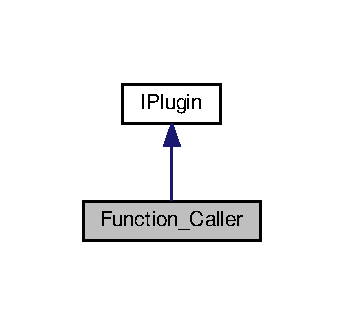
\includegraphics[width=165pt]{class_function___caller__inherit__graph}
\end{center}
\end{figure}


Collaboration diagram for Function\+\_\+\+Caller\+:\nopagebreak
\begin{figure}[H]
\begin{center}
\leavevmode
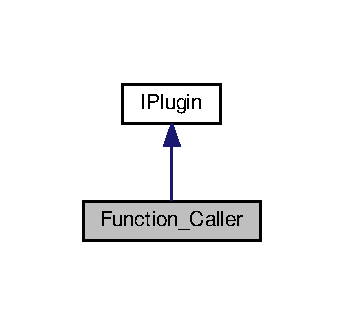
\includegraphics[width=165pt]{class_function___caller__coll__graph}
\end{center}
\end{figure}
\subsection*{Public Member Functions}
\begin{DoxyCompactItemize}
\item 
void \hyperlink{class_function___caller_a4c39451baadbdc89f6f7e212638cb811}{Main} ()
\begin{DoxyCompactList}\small\item\em Main funcction of the plugin. \end{DoxyCompactList}\item 
bool \hyperlink{class_function___caller_a6ce3a356b5eb30c51d39f2ce0ecb9128}{load\+Configuration} ()
\begin{DoxyCompactList}\small\item\em Load configuration. \end{DoxyCompactList}\item 
bool \hyperlink{class_function___caller_a639edde2994f2317a922c2a80083ce54}{save\+Configuration} ()
\begin{DoxyCompactList}\small\item\em Save configuration. \end{DoxyCompactList}\item 
bool \hyperlink{class_function___caller_a6499f7bae56266b6372351da555f316f}{Initialize\+\_\+\+Output} ()
\begin{DoxyCompactList}\small\item\em Initialize Output variables for the plugin to publish. \end{DoxyCompactList}\item 
bool \hyperlink{class_function___caller_a9b879313b891d3e60b105f94e3fd71cf}{Initialize\+\_\+\+Input} ()
\begin{DoxyCompactList}\small\item\em Initialize Input variables for the plugin to publish. \end{DoxyCompactList}\item 
void \hyperlink{class_function___caller_af099d310156da34103de5486995b00e2}{stop} ()
\begin{DoxyCompactList}\small\item\em Stop plugin. \end{DoxyCompactList}\item 
void \hyperlink{class_function___caller_a508165a2fab0cb3f77d89135994f342d}{run} ()
\begin{DoxyCompactList}\small\item\em Execute plugin. \end{DoxyCompactList}\end{DoxyCompactItemize}
\subsection*{Additional Inherited Members}


\subsection{Detailed Description}
\hyperlink{class_function___caller}{Function\+\_\+\+Caller} plugin. 

This plugin is a test to add function calls to the \hyperlink{class_shared___memory}{Shared\+\_\+\+Memory}, the functions have 2 std\+::vectors string as parameters. Each function is responsible for parsing the imput to map it to shared variables \begin{DoxyAuthor}{Author}
Patrick Heyer, \href{mailto:patrickhey@prodigy.net.mx}{\tt patrickhey@prodigy.\+net.\+mx} 
\end{DoxyAuthor}
\begin{DoxyDate}{Date}
jul 13, 2014 
\end{DoxyDate}
\begin{DoxyVersion}{Version}
1.\+0 
\end{DoxyVersion}


Definition at line 14 of file Function\+\_\+\+Caller.\+h.



\subsection{Member Function Documentation}
\mbox{\Hypertarget{class_function___caller_a9b879313b891d3e60b105f94e3fd71cf}\label{class_function___caller_a9b879313b891d3e60b105f94e3fd71cf}} 
\index{Function\+\_\+\+Caller@{Function\+\_\+\+Caller}!Initialize\+\_\+\+Input@{Initialize\+\_\+\+Input}}
\index{Initialize\+\_\+\+Input@{Initialize\+\_\+\+Input}!Function\+\_\+\+Caller@{Function\+\_\+\+Caller}}
\subsubsection{\texorpdfstring{Initialize\+\_\+\+Input()}{Initialize\_Input()}}
{\footnotesize\ttfamily bool Function\+\_\+\+Caller\+::\+Initialize\+\_\+\+Input (\begin{DoxyParamCaption}{ }\end{DoxyParamCaption})\hspace{0.3cm}{\ttfamily [virtual]}}



Initialize Input variables for the plugin to publish. 

\begin{DoxyReturn}{Returns}
bool 
\end{DoxyReturn}


Implements \hyperlink{class_i_plugin_aa7c66743ad956d8ada57becee559af4d}{I\+Plugin}.



Definition at line 91 of file Main.\+cpp.


\begin{DoxyCode}
92 \{
93     empty\_call = Shared\_Memory::getInstance().Register\_Func\_Input(\textcolor{stringliteral}{"published\_empty\_function"});
94     input\_call = Shared\_Memory::getInstance().Register\_Func\_Input(\textcolor{stringliteral}{"published\_input\_function"});
95     output\_call = Shared\_Memory::getInstance().Register\_Func\_Input(\textcolor{stringliteral}{"published\_output\_function"});
96     IO\_call = Shared\_Memory::getInstance().Register\_Func\_Input(\textcolor{stringliteral}{"published\_IO\_function"});
97     \textcolor{keywordflow}{return} \textcolor{keyword}{true};
98 \}
\end{DoxyCode}
\mbox{\Hypertarget{class_function___caller_a6499f7bae56266b6372351da555f316f}\label{class_function___caller_a6499f7bae56266b6372351da555f316f}} 
\index{Function\+\_\+\+Caller@{Function\+\_\+\+Caller}!Initialize\+\_\+\+Output@{Initialize\+\_\+\+Output}}
\index{Initialize\+\_\+\+Output@{Initialize\+\_\+\+Output}!Function\+\_\+\+Caller@{Function\+\_\+\+Caller}}
\subsubsection{\texorpdfstring{Initialize\+\_\+\+Output()}{Initialize\_Output()}}
{\footnotesize\ttfamily bool Function\+\_\+\+Caller\+::\+Initialize\+\_\+\+Output (\begin{DoxyParamCaption}{ }\end{DoxyParamCaption})\hspace{0.3cm}{\ttfamily [virtual]}}



Initialize Output variables for the plugin to publish. 

\begin{DoxyReturn}{Returns}
bool 
\end{DoxyReturn}


Implements \hyperlink{class_i_plugin_a0b772513fc8c4ed01240e19c4bb84068}{I\+Plugin}.



Definition at line 85 of file Main.\+cpp.


\begin{DoxyCode}
86 \{
87 
88     \textcolor{keywordflow}{return} \textcolor{keyword}{true};
89 \}
\end{DoxyCode}
\mbox{\Hypertarget{class_function___caller_a6ce3a356b5eb30c51d39f2ce0ecb9128}\label{class_function___caller_a6ce3a356b5eb30c51d39f2ce0ecb9128}} 
\index{Function\+\_\+\+Caller@{Function\+\_\+\+Caller}!load\+Configuration@{load\+Configuration}}
\index{load\+Configuration@{load\+Configuration}!Function\+\_\+\+Caller@{Function\+\_\+\+Caller}}
\subsubsection{\texorpdfstring{load\+Configuration()}{loadConfiguration()}}
{\footnotesize\ttfamily bool Function\+\_\+\+Caller\+::load\+Configuration (\begin{DoxyParamCaption}{ }\end{DoxyParamCaption})\hspace{0.3cm}{\ttfamily [virtual]}}



Load configuration. 

The configuration can be loaded from file, or be hard coded into the plugin (not recomended), initialization of public and private variables should occur here

By default load\+Configuration is called during \hyperlink{class_plugin_manager_a956e653b7db36da9d034b4a93c8308d5}{Plugin\+Manager\+::\+Initialize()} by the plugin manager.

\begin{DoxyReturn}{Returns}
bool 
\end{DoxyReturn}


Implements \hyperlink{class_i_plugin_a418cff309436d3a15d9a4ce7369db6dd}{I\+Plugin}.



Definition at line 75 of file Main.\+cpp.


\begin{DoxyCode}
76 \{
77     \textcolor{keywordflow}{return} \textcolor{keyword}{true};
78 \}
\end{DoxyCode}
\mbox{\Hypertarget{class_function___caller_a4c39451baadbdc89f6f7e212638cb811}\label{class_function___caller_a4c39451baadbdc89f6f7e212638cb811}} 
\index{Function\+\_\+\+Caller@{Function\+\_\+\+Caller}!Main@{Main}}
\index{Main@{Main}!Function\+\_\+\+Caller@{Function\+\_\+\+Caller}}
\subsubsection{\texorpdfstring{Main()}{Main()}}
{\footnotesize\ttfamily void Function\+\_\+\+Caller\+::\+Main (\begin{DoxyParamCaption}{ }\end{DoxyParamCaption})\hspace{0.3cm}{\ttfamily [virtual]}}



Main funcction of the plugin. 

Started in a new thread by the Run() funcction is the most importatn funcction of the plugin. Infinite loop (generaly a while(running) function that runs undefenitly in a read/process/write cicle). \begin{DoxyReturn}{Returns}
void 
\end{DoxyReturn}


Implements \hyperlink{class_i_plugin_ab5fdb3b0f7afdcee04324dca01766749}{I\+Plugin}.



Definition at line 53 of file Main.\+cpp.


\begin{DoxyCode}
54 \{
55     std::vector<std::string> i\_empty;
56     std::vector<std::string> o\_empty;
57     std::vector<std::string> i\_input= \{\textcolor{stringliteral}{"INPUT\_1"}, \textcolor{stringliteral}{"INPUT\_2"}, \textcolor{stringliteral}{"INPUT\_3"}, \textcolor{stringliteral}{"INPUT\_4"}\};
58     std::vector<std::string> o\_input= \{\textcolor{stringliteral}{"OUTPUT\_1"}, \textcolor{stringliteral}{"OUTPUT\_2"}, \textcolor{stringliteral}{"OUTPUT\_3"}, \textcolor{stringliteral}{"OUTPUT\_4"}\};
59     
60     \textcolor{keywordflow}{for}(\textcolor{keywordtype}{int} o=0; o<10000; o++)
61     \{
62         usleep(500);
63     \}
64     
65     empty\_call(i\_empty,o\_empty);
66     input\_call(i\_input,o\_empty);
67     output\_call(i\_empty,o\_input);
68     IO\_call(i\_input,o\_input);
69 
70     stoped=\textcolor{keyword}{true};
71     \textcolor{keywordflow}{return};
72 \}
\end{DoxyCode}
\mbox{\Hypertarget{class_function___caller_a508165a2fab0cb3f77d89135994f342d}\label{class_function___caller_a508165a2fab0cb3f77d89135994f342d}} 
\index{Function\+\_\+\+Caller@{Function\+\_\+\+Caller}!run@{run}}
\index{run@{run}!Function\+\_\+\+Caller@{Function\+\_\+\+Caller}}
\subsubsection{\texorpdfstring{run()}{run()}}
{\footnotesize\ttfamily void Function\+\_\+\+Caller\+::run (\begin{DoxyParamCaption}{ }\end{DoxyParamCaption})\hspace{0.3cm}{\ttfamily [virtual]}}



Execute plugin. 

Starts a new thread and executes the plugins main() funcction. \begin{DoxyReturn}{Returns}
void 
\end{DoxyReturn}


Implements \hyperlink{class_i_plugin_a46b4ace767e77f9db9c9585e99c09039}{I\+Plugin}.



Definition at line 99 of file Main.\+cpp.



References I\+Plugin\+::\+Inc\+Wrapper().


\begin{DoxyCode}
100 \{
101     pthread\_create(&thread\_id, NULL, &\hyperlink{class_i_plugin_a62d22be2fdf66eb7f5c2f797f5f3d7f3}{IPlugin::IncWrapper}, \textcolor{keyword}{this});
102     running = \textcolor{keyword}{true};
103     stoped = \textcolor{keyword}{false};
104 \}
\end{DoxyCode}
\mbox{\Hypertarget{class_function___caller_a639edde2994f2317a922c2a80083ce54}\label{class_function___caller_a639edde2994f2317a922c2a80083ce54}} 
\index{Function\+\_\+\+Caller@{Function\+\_\+\+Caller}!save\+Configuration@{save\+Configuration}}
\index{save\+Configuration@{save\+Configuration}!Function\+\_\+\+Caller@{Function\+\_\+\+Caller}}
\subsubsection{\texorpdfstring{save\+Configuration()}{saveConfiguration()}}
{\footnotesize\ttfamily bool Function\+\_\+\+Caller\+::save\+Configuration (\begin{DoxyParamCaption}{ }\end{DoxyParamCaption})\hspace{0.3cm}{\ttfamily [virtual]}}



Save configuration. 

The configuration should be saved to file, public and private variables that should be configured at startup should be saved.

By default save\+Configuration is called during \hyperlink{class_plugin_manager_ab651a05d6fcb92562807e9f5ecc30855}{Plugin\+Manager\+::\+Unload()} by the plugin manager.

\begin{DoxyReturn}{Returns}
bool 
\end{DoxyReturn}


Implements \hyperlink{class_i_plugin_a79b5c42b1c7b08257a6110b2091039bc}{I\+Plugin}.



Definition at line 80 of file Main.\+cpp.


\begin{DoxyCode}
81 \{
82     \textcolor{keywordflow}{return} \textcolor{keyword}{true};
83 \}
\end{DoxyCode}
\mbox{\Hypertarget{class_function___caller_af099d310156da34103de5486995b00e2}\label{class_function___caller_af099d310156da34103de5486995b00e2}} 
\index{Function\+\_\+\+Caller@{Function\+\_\+\+Caller}!stop@{stop}}
\index{stop@{stop}!Function\+\_\+\+Caller@{Function\+\_\+\+Caller}}
\subsubsection{\texorpdfstring{stop()}{stop()}}
{\footnotesize\ttfamily void Function\+\_\+\+Caller\+::stop (\begin{DoxyParamCaption}{ }\end{DoxyParamCaption})\hspace{0.3cm}{\ttfamily [virtual]}}



Stop plugin. 

Stops the plugin \begin{DoxyReturn}{Returns}
void 
\end{DoxyReturn}


Implements \hyperlink{class_i_plugin_a86e523c283aec5c9fb21249a76e916ac}{I\+Plugin}.



Definition at line 106 of file Main.\+cpp.


\begin{DoxyCode}
107 \{
108     running = \textcolor{keyword}{false};
109 \}
\end{DoxyCode}


The documentation for this class was generated from the following files\+:\begin{DoxyCompactItemize}
\item 
/home/patrick/projects/\+Gesture\+\_\+\+Therapy\+\_\+\+Linux/src/\+Function\+\_\+\+Caller/Function\+\_\+\+Caller.\+h\item 
/home/patrick/projects/\+Gesture\+\_\+\+Therapy\+\_\+\+Linux/src/\+Function\+\_\+\+Caller/Main.\+cpp\end{DoxyCompactItemize}

\hypertarget{class_function___test}{}\section{Function\+\_\+\+Test Class Reference}
\label{class_function___test}\index{Function\+\_\+\+Test@{Function\+\_\+\+Test}}


\hyperlink{class_function___test}{Function\+\_\+\+Test} plugin.  




{\ttfamily \#include $<$Function\+\_\+\+Test.\+h$>$}



Inheritance diagram for Function\+\_\+\+Test\+:\nopagebreak
\begin{figure}[H]
\begin{center}
\leavevmode
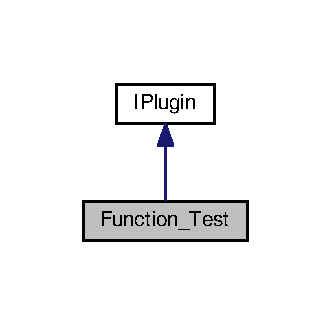
\includegraphics[width=159pt]{class_function___test__inherit__graph}
\end{center}
\end{figure}


Collaboration diagram for Function\+\_\+\+Test\+:\nopagebreak
\begin{figure}[H]
\begin{center}
\leavevmode
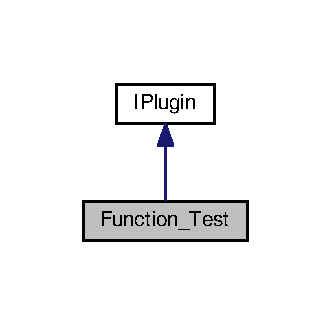
\includegraphics[width=159pt]{class_function___test__coll__graph}
\end{center}
\end{figure}
\subsection*{Public Member Functions}
\begin{DoxyCompactItemize}
\item 
void \hyperlink{class_function___test_a87d81cc4014216aa2523ef69c5b35dff}{Main} ()
\begin{DoxyCompactList}\small\item\em Main funcction of the plugin. \end{DoxyCompactList}\item 
bool \hyperlink{class_function___test_ab2f00495eb55e7edf061498dcf7aaa4f}{load\+Configuration} ()
\begin{DoxyCompactList}\small\item\em Load configuration. \end{DoxyCompactList}\item 
bool \hyperlink{class_function___test_a6d8832ce28b9b659c85db0e32183abc9}{save\+Configuration} ()
\begin{DoxyCompactList}\small\item\em Save configuration. \end{DoxyCompactList}\item 
bool \hyperlink{class_function___test_afffb9c39e5b1178774cc3a1191124409}{Initialize\+\_\+\+Output} ()
\begin{DoxyCompactList}\small\item\em Initialize Output variables for the plugin to publish. \end{DoxyCompactList}\item 
bool \hyperlink{class_function___test_a4d937dda611ec1b3bbdd70cdad6d76d2}{Initialize\+\_\+\+Input} ()
\begin{DoxyCompactList}\small\item\em Initialize Input variables for the plugin to publish. \end{DoxyCompactList}\item 
void \hyperlink{class_function___test_ac4a090ec1f44393fc7a8e851cb76fb29}{stop} ()
\begin{DoxyCompactList}\small\item\em Stop plugin. \end{DoxyCompactList}\item 
void \hyperlink{class_function___test_ae9c552f668d5f2dad706677908d9e623}{run} ()
\begin{DoxyCompactList}\small\item\em Execute plugin. \end{DoxyCompactList}\end{DoxyCompactItemize}
\subsection*{Additional Inherited Members}


\subsection{Detailed Description}
\hyperlink{class_function___test}{Function\+\_\+\+Test} plugin. 

This plugin is a test to add function calls to the \hyperlink{class_shared___memory}{Shared\+\_\+\+Memory}, the functions have 2 std\+::vectors string as parameters. Each function is responsible for parsing the imput to map it to shared variables \begin{DoxyAuthor}{Author}
Patrick Heyer, \href{mailto:patrickhey@prodigy.net.mx}{\tt patrickhey@prodigy.\+net.\+mx} 
\end{DoxyAuthor}
\begin{DoxyDate}{Date}
jul 13, 2014 
\end{DoxyDate}
\begin{DoxyVersion}{Version}
1.\+0 
\end{DoxyVersion}


Definition at line 14 of file Function\+\_\+\+Test.\+h.



\subsection{Member Function Documentation}
\mbox{\Hypertarget{class_function___test_a4d937dda611ec1b3bbdd70cdad6d76d2}\label{class_function___test_a4d937dda611ec1b3bbdd70cdad6d76d2}} 
\index{Function\+\_\+\+Test@{Function\+\_\+\+Test}!Initialize\+\_\+\+Input@{Initialize\+\_\+\+Input}}
\index{Initialize\+\_\+\+Input@{Initialize\+\_\+\+Input}!Function\+\_\+\+Test@{Function\+\_\+\+Test}}
\subsubsection{\texorpdfstring{Initialize\+\_\+\+Input()}{Initialize\_Input()}}
{\footnotesize\ttfamily bool Function\+\_\+\+Test\+::\+Initialize\+\_\+\+Input (\begin{DoxyParamCaption}{ }\end{DoxyParamCaption})\hspace{0.3cm}{\ttfamily [virtual]}}



Initialize Input variables for the plugin to publish. 

\begin{DoxyReturn}{Returns}
bool 
\end{DoxyReturn}


Implements \hyperlink{class_i_plugin_aa7c66743ad956d8ada57becee559af4d}{I\+Plugin}.



Definition at line 138 of file Main.\+cpp.


\begin{DoxyCode}
139 \{
140     \textcolor{keywordflow}{return} \textcolor{keyword}{true};
141 \}
\end{DoxyCode}
\mbox{\Hypertarget{class_function___test_afffb9c39e5b1178774cc3a1191124409}\label{class_function___test_afffb9c39e5b1178774cc3a1191124409}} 
\index{Function\+\_\+\+Test@{Function\+\_\+\+Test}!Initialize\+\_\+\+Output@{Initialize\+\_\+\+Output}}
\index{Initialize\+\_\+\+Output@{Initialize\+\_\+\+Output}!Function\+\_\+\+Test@{Function\+\_\+\+Test}}
\subsubsection{\texorpdfstring{Initialize\+\_\+\+Output()}{Initialize\_Output()}}
{\footnotesize\ttfamily bool Function\+\_\+\+Test\+::\+Initialize\+\_\+\+Output (\begin{DoxyParamCaption}{ }\end{DoxyParamCaption})\hspace{0.3cm}{\ttfamily [virtual]}}



Initialize Output variables for the plugin to publish. 

\begin{DoxyReturn}{Returns}
bool 
\end{DoxyReturn}


Implements \hyperlink{class_i_plugin_a0b772513fc8c4ed01240e19c4bb84068}{I\+Plugin}.



Definition at line 122 of file Main.\+cpp.


\begin{DoxyCode}
123 \{
124     std::function<void(std::vector<std::string> i\_params, std::vector<std::string> o\_params)> 
      published\_empty = empty\_function;
125     Shared\_Memory::getInstance().Register\_Output(\textcolor{stringliteral}{"published\_empty\_function"}, published\_empty);
126     
127     std::function<void(std::vector<std::string> i\_params, std::vector<std::string> o\_params)> 
      published\_input = input\_function;
128     Shared\_Memory::getInstance().Register\_Output(\textcolor{stringliteral}{"published\_input\_function"}, published\_input);
129     
130     std::function<void(std::vector<std::string> i\_params, std::vector<std::string> o\_params)> 
      published\_output = output\_function;
131     Shared\_Memory::getInstance().Register\_Output(\textcolor{stringliteral}{"published\_output\_function"}, published\_output);
132     
133     std::function<void(std::vector<std::string> i\_params, std::vector<std::string> o\_params)> published\_IO 
      = IO\_function;
134     Shared\_Memory::getInstance().Register\_Output(\textcolor{stringliteral}{"published\_IO\_function"}, published\_IO);
135     \textcolor{keywordflow}{return} \textcolor{keyword}{true};
136 \}
\end{DoxyCode}
\mbox{\Hypertarget{class_function___test_ab2f00495eb55e7edf061498dcf7aaa4f}\label{class_function___test_ab2f00495eb55e7edf061498dcf7aaa4f}} 
\index{Function\+\_\+\+Test@{Function\+\_\+\+Test}!load\+Configuration@{load\+Configuration}}
\index{load\+Configuration@{load\+Configuration}!Function\+\_\+\+Test@{Function\+\_\+\+Test}}
\subsubsection{\texorpdfstring{load\+Configuration()}{loadConfiguration()}}
{\footnotesize\ttfamily bool Function\+\_\+\+Test\+::load\+Configuration (\begin{DoxyParamCaption}{ }\end{DoxyParamCaption})\hspace{0.3cm}{\ttfamily [virtual]}}



Load configuration. 

The configuration can be loaded from file, or be hard coded into the plugin (not recomended), initialization of public and private variables should occur here

By default load\+Configuration is called during \hyperlink{class_plugin_manager_a956e653b7db36da9d034b4a93c8308d5}{Plugin\+Manager\+::\+Initialize()} by the plugin manager.

\begin{DoxyReturn}{Returns}
bool 
\end{DoxyReturn}


Implements \hyperlink{class_i_plugin_a418cff309436d3a15d9a4ce7369db6dd}{I\+Plugin}.



Definition at line 112 of file Main.\+cpp.


\begin{DoxyCode}
113 \{
114     \textcolor{keywordflow}{return} \textcolor{keyword}{true};
115 \}
\end{DoxyCode}
\mbox{\Hypertarget{class_function___test_a87d81cc4014216aa2523ef69c5b35dff}\label{class_function___test_a87d81cc4014216aa2523ef69c5b35dff}} 
\index{Function\+\_\+\+Test@{Function\+\_\+\+Test}!Main@{Main}}
\index{Main@{Main}!Function\+\_\+\+Test@{Function\+\_\+\+Test}}
\subsubsection{\texorpdfstring{Main()}{Main()}}
{\footnotesize\ttfamily void Function\+\_\+\+Test\+::\+Main (\begin{DoxyParamCaption}{ }\end{DoxyParamCaption})\hspace{0.3cm}{\ttfamily [virtual]}}



Main funcction of the plugin. 

Started in a new thread by the Run() funcction is the most importatn funcction of the plugin. Infinite loop (generaly a while(running) function that runs undefenitly in a read/process/write cicle). \begin{DoxyReturn}{Returns}
void 
\end{DoxyReturn}


Implements \hyperlink{class_i_plugin_ab5fdb3b0f7afdcee04324dca01766749}{I\+Plugin}.



Definition at line 107 of file Main.\+cpp.


\begin{DoxyCode}
108 \{
109     \textcolor{keywordflow}{return};
110 \}
\end{DoxyCode}
\mbox{\Hypertarget{class_function___test_ae9c552f668d5f2dad706677908d9e623}\label{class_function___test_ae9c552f668d5f2dad706677908d9e623}} 
\index{Function\+\_\+\+Test@{Function\+\_\+\+Test}!run@{run}}
\index{run@{run}!Function\+\_\+\+Test@{Function\+\_\+\+Test}}
\subsubsection{\texorpdfstring{run()}{run()}}
{\footnotesize\ttfamily void Function\+\_\+\+Test\+::run (\begin{DoxyParamCaption}{ }\end{DoxyParamCaption})\hspace{0.3cm}{\ttfamily [virtual]}}



Execute plugin. 

Starts a new thread and executes the plugins main() funcction. \begin{DoxyReturn}{Returns}
void 
\end{DoxyReturn}


Implements \hyperlink{class_i_plugin_a46b4ace767e77f9db9c9585e99c09039}{I\+Plugin}.



Definition at line 142 of file Main.\+cpp.


\begin{DoxyCode}
143 \{
144     stoped = \textcolor{keyword}{true};
145 \}
\end{DoxyCode}
\mbox{\Hypertarget{class_function___test_a6d8832ce28b9b659c85db0e32183abc9}\label{class_function___test_a6d8832ce28b9b659c85db0e32183abc9}} 
\index{Function\+\_\+\+Test@{Function\+\_\+\+Test}!save\+Configuration@{save\+Configuration}}
\index{save\+Configuration@{save\+Configuration}!Function\+\_\+\+Test@{Function\+\_\+\+Test}}
\subsubsection{\texorpdfstring{save\+Configuration()}{saveConfiguration()}}
{\footnotesize\ttfamily bool Function\+\_\+\+Test\+::save\+Configuration (\begin{DoxyParamCaption}{ }\end{DoxyParamCaption})\hspace{0.3cm}{\ttfamily [virtual]}}



Save configuration. 

The configuration should be saved to file, public and private variables that should be configured at startup should be saved.

By default save\+Configuration is called during \hyperlink{class_plugin_manager_ab651a05d6fcb92562807e9f5ecc30855}{Plugin\+Manager\+::\+Unload()} by the plugin manager.

\begin{DoxyReturn}{Returns}
bool 
\end{DoxyReturn}


Implements \hyperlink{class_i_plugin_a79b5c42b1c7b08257a6110b2091039bc}{I\+Plugin}.



Definition at line 117 of file Main.\+cpp.


\begin{DoxyCode}
118 \{
119     \textcolor{keywordflow}{return} \textcolor{keyword}{true};
120 \}
\end{DoxyCode}
\mbox{\Hypertarget{class_function___test_ac4a090ec1f44393fc7a8e851cb76fb29}\label{class_function___test_ac4a090ec1f44393fc7a8e851cb76fb29}} 
\index{Function\+\_\+\+Test@{Function\+\_\+\+Test}!stop@{stop}}
\index{stop@{stop}!Function\+\_\+\+Test@{Function\+\_\+\+Test}}
\subsubsection{\texorpdfstring{stop()}{stop()}}
{\footnotesize\ttfamily void Function\+\_\+\+Test\+::stop (\begin{DoxyParamCaption}{ }\end{DoxyParamCaption})\hspace{0.3cm}{\ttfamily [virtual]}}



Stop plugin. 

Stops the plugin \begin{DoxyReturn}{Returns}
void 
\end{DoxyReturn}


Implements \hyperlink{class_i_plugin_a86e523c283aec5c9fb21249a76e916ac}{I\+Plugin}.



Definition at line 147 of file Main.\+cpp.


\begin{DoxyCode}
148 \{
149     running = \textcolor{keyword}{false};
150 \}
\end{DoxyCode}


The documentation for this class was generated from the following files\+:\begin{DoxyCompactItemize}
\item 
/home/patrick/projects/\+Gesture\+\_\+\+Therapy\+\_\+\+Linux/src/\+Function\+\_\+\+Test/Function\+\_\+\+Test.\+h\item 
/home/patrick/projects/\+Gesture\+\_\+\+Therapy\+\_\+\+Linux/src/\+Function\+\_\+\+Test/Main.\+cpp\end{DoxyCompactItemize}

\hypertarget{class_plugin_instance_1_1_impl}{}\section{Plugin\+Instance\+:\+:Impl Class Reference}
\label{class_plugin_instance_1_1_impl}\index{Plugin\+Instance\+::\+Impl@{Plugin\+Instance\+::\+Impl}}


Collaboration diagram for Plugin\+Instance\+:\+:Impl\+:\nopagebreak
\begin{figure}[H]
\begin{center}
\leavevmode
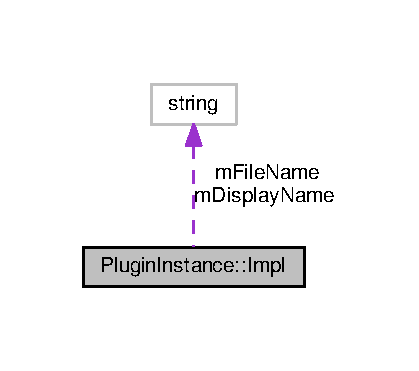
\includegraphics[width=201pt]{class_plugin_instance_1_1_impl__coll__graph}
\end{center}
\end{figure}
\subsection*{Public Types}
\begin{DoxyCompactItemize}
\item 
\mbox{\Hypertarget{class_plugin_instance_1_1_impl_a03b4108cd0fcdd2fb9b3309b1287b19d}\label{class_plugin_instance_1_1_impl_a03b4108cd0fcdd2fb9b3309b1287b19d}} 
typedef void($\ast$ {\bfseries Plugin\+Func}) ()
\end{DoxyCompactItemize}
\subsection*{Public Member Functions}
\begin{DoxyCompactItemize}
\item 
\mbox{\Hypertarget{class_plugin_instance_1_1_impl_a26ed51baaf9ab8c93406fa904680f964}\label{class_plugin_instance_1_1_impl_a26ed51baaf9ab8c93406fa904680f964}} 
bool {\bfseries Load} ()
\item 
\mbox{\Hypertarget{class_plugin_instance_1_1_impl_a0d52897125a93cc6ebf60d3f92f60434}\label{class_plugin_instance_1_1_impl_a0d52897125a93cc6ebf60d3f92f60434}} 
bool {\bfseries Unload} ()
\item 
\mbox{\Hypertarget{class_plugin_instance_1_1_impl_a9266ef053cc13f8115ec56e900bf6742}\label{class_plugin_instance_1_1_impl_a9266ef053cc13f8115ec56e900bf6742}} 
Plugin\+Func {\bfseries Get\+Function} (const std\+::string \&name)
\end{DoxyCompactItemize}
\subsection*{Public Attributes}
\begin{DoxyCompactItemize}
\item 
\mbox{\Hypertarget{class_plugin_instance_1_1_impl_a8bc5c813f43b69836978cca9bdd9ac5d}\label{class_plugin_instance_1_1_impl_a8bc5c813f43b69836978cca9bdd9ac5d}} 
std\+::string {\bfseries m\+File\+Name}
\item 
\mbox{\Hypertarget{class_plugin_instance_1_1_impl_a834bb1cd6c65432f8e2764f2f922dc89}\label{class_plugin_instance_1_1_impl_a834bb1cd6c65432f8e2764f2f922dc89}} 
std\+::string {\bfseries m\+Display\+Name}
\item 
\mbox{\Hypertarget{class_plugin_instance_1_1_impl_aff0dafb151cc128f05914b2838a8fa1f}\label{class_plugin_instance_1_1_impl_aff0dafb151cc128f05914b2838a8fa1f}} 
void $\ast$ {\bfseries handle}
\end{DoxyCompactItemize}


\subsection{Detailed Description}


Definition at line 23 of file pluginmanager.\+cpp.



The documentation for this class was generated from the following file\+:\begin{DoxyCompactItemize}
\item 
/home/patrick/projects/\+Gesture\+\_\+\+Therapy\+\_\+\+Linux/src/\+Plugin\+\_\+\+A\+P\+I/pluginmanager.\+cpp\end{DoxyCompactItemize}

\hypertarget{class_i_plugin}{}\section{I\+Plugin Class Reference}
\label{class_i_plugin}\index{I\+Plugin@{I\+Plugin}}


{\ttfamily \#include $<$plugin.\+h$>$}



Inheritance diagram for I\+Plugin\+:\nopagebreak
\begin{figure}[H]
\begin{center}
\leavevmode
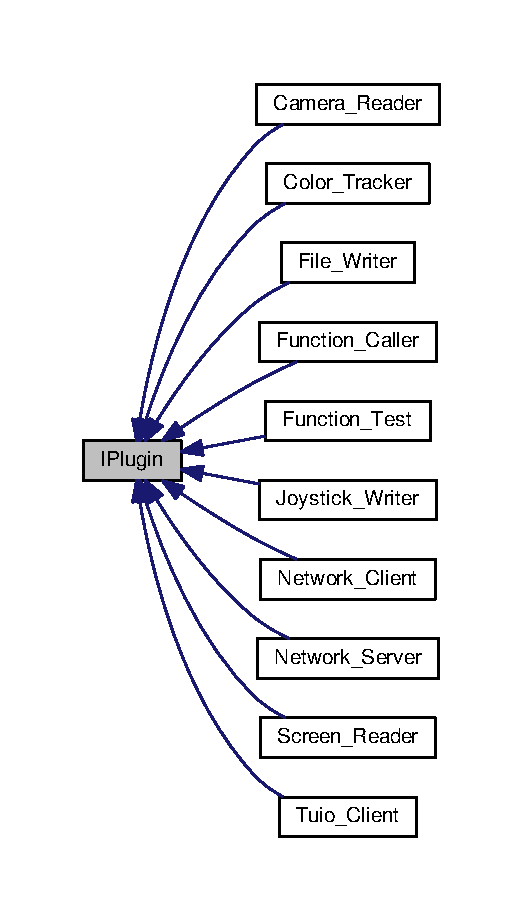
\includegraphics[width=251pt]{class_i_plugin__inherit__graph}
\end{center}
\end{figure}
\subsection*{Public Member Functions}
\begin{DoxyCompactItemize}
\item 
virtual bool \hyperlink{class_i_plugin_a0b772513fc8c4ed01240e19c4bb84068}{Initialize\+\_\+\+Output} ()=0
\begin{DoxyCompactList}\small\item\em Initialize Output variables for the plugin to publish. \end{DoxyCompactList}\item 
virtual bool \hyperlink{class_i_plugin_aa7c66743ad956d8ada57becee559af4d}{Initialize\+\_\+\+Input} ()=0
\begin{DoxyCompactList}\small\item\em Initialize Input variables for the plugin to publish. \end{DoxyCompactList}\item 
virtual void \hyperlink{class_i_plugin_ab5fdb3b0f7afdcee04324dca01766749}{Main} ()=0
\begin{DoxyCompactList}\small\item\em Main funcction of the plugin. \end{DoxyCompactList}\item 
virtual bool \hyperlink{class_i_plugin_a418cff309436d3a15d9a4ce7369db6dd}{load\+Configuration} ()=0
\begin{DoxyCompactList}\small\item\em Load configuration. \end{DoxyCompactList}\item 
virtual bool \hyperlink{class_i_plugin_a79b5c42b1c7b08257a6110b2091039bc}{save\+Configuration} ()=0
\begin{DoxyCompactList}\small\item\em Save configuration. \end{DoxyCompactList}\item 
virtual void \hyperlink{class_i_plugin_a46b4ace767e77f9db9c9585e99c09039}{run} ()=0
\begin{DoxyCompactList}\small\item\em Execute plugin. \end{DoxyCompactList}\item 
virtual void \hyperlink{class_i_plugin_a86e523c283aec5c9fb21249a76e916ac}{stop} ()=0
\begin{DoxyCompactList}\small\item\em Stop plugin. \end{DoxyCompactList}\end{DoxyCompactItemize}
\subsection*{Static Public Member Functions}
\begin{DoxyCompactItemize}
\item 
static void $\ast$ \hyperlink{class_i_plugin_a62d22be2fdf66eb7f5c2f797f5f3d7f3}{Inc\+Wrapper} (void $\ast$this\+Ptr)
\begin{DoxyCompactList}\small\item\em Wrapps the Main function of the plugin object to A\+N\+SI C to be pased as a parameter to pthread\+\_\+create. \end{DoxyCompactList}\end{DoxyCompactItemize}
\subsection*{Public Attributes}
\begin{DoxyCompactItemize}
\item 
\mbox{\Hypertarget{class_i_plugin_a2b6bd7ba10e171049c50cfee4f7510b4}\label{class_i_plugin_a2b6bd7ba10e171049c50cfee4f7510b4}} 
pthread\+\_\+t {\bfseries thread\+\_\+id}
\item 
\mbox{\Hypertarget{class_i_plugin_ae20c05c87269f8d66a50d6995dfb3f66}\label{class_i_plugin_ae20c05c87269f8d66a50d6995dfb3f66}} 
bool {\bfseries running}
\item 
\mbox{\Hypertarget{class_i_plugin_a9a89c705a50372eb079ac8e6f7a9286a}\label{class_i_plugin_a9a89c705a50372eb079ac8e6f7a9286a}} 
bool {\bfseries stoped}
\end{DoxyCompactItemize}


\subsection{Detailed Description}
An abstract interface for plugins to create new plugins. 

Definition at line 18 of file plugin.\+h.



\subsection{Member Function Documentation}
\mbox{\Hypertarget{class_i_plugin_a62d22be2fdf66eb7f5c2f797f5f3d7f3}\label{class_i_plugin_a62d22be2fdf66eb7f5c2f797f5f3d7f3}} 
\index{I\+Plugin@{I\+Plugin}!Inc\+Wrapper@{Inc\+Wrapper}}
\index{Inc\+Wrapper@{Inc\+Wrapper}!I\+Plugin@{I\+Plugin}}
\subsubsection{\texorpdfstring{Inc\+Wrapper()}{IncWrapper()}}
{\footnotesize\ttfamily static void$\ast$ I\+Plugin\+::\+Inc\+Wrapper (\begin{DoxyParamCaption}\item[{void $\ast$}]{this\+Ptr }\end{DoxyParamCaption})\hspace{0.3cm}{\ttfamily [inline]}, {\ttfamily [static]}}



Wrapps the Main function of the plugin object to A\+N\+SI C to be pased as a parameter to pthread\+\_\+create. 

This process alows plugins to be running in a new thread each (don\textquotesingle{}t change this unless you know what you are doing)

\begin{DoxyReturn}{Returns}
static void 
\end{DoxyReturn}


Definition at line 94 of file plugin.\+h.



Referenced by Color\+\_\+\+Tracker\+::run(), File\+\_\+\+Writer\+::run(), Function\+\_\+\+Caller\+::run(), Camera\+\_\+\+Reader\+::run(), Joystick\+\_\+\+Writer\+::run(), Network\+\_\+\+Client\+::run(), Network\+\_\+\+Server\+::run(), Screen\+\_\+\+Reader\+::run(), and Tuio\+\_\+\+Client\+::run().


\begin{DoxyCode}
95     \{
96       ((\hyperlink{class_i_plugin}{IPlugin}*) thisPtr)->Main();
97       \textcolor{keywordflow}{return} NULL;
98     \}
\end{DoxyCode}
\mbox{\Hypertarget{class_i_plugin_aa7c66743ad956d8ada57becee559af4d}\label{class_i_plugin_aa7c66743ad956d8ada57becee559af4d}} 
\index{I\+Plugin@{I\+Plugin}!Initialize\+\_\+\+Input@{Initialize\+\_\+\+Input}}
\index{Initialize\+\_\+\+Input@{Initialize\+\_\+\+Input}!I\+Plugin@{I\+Plugin}}
\subsubsection{\texorpdfstring{Initialize\+\_\+\+Input()}{Initialize\_Input()}}
{\footnotesize\ttfamily virtual bool I\+Plugin\+::\+Initialize\+\_\+\+Input (\begin{DoxyParamCaption}{ }\end{DoxyParamCaption})\hspace{0.3cm}{\ttfamily [pure virtual]}}



Initialize Input variables for the plugin to publish. 

\begin{DoxyReturn}{Returns}
bool 
\end{DoxyReturn}


Implemented in \hyperlink{class_tuio___client_a66bd1d9dc23405e7589d899ef6c5d892}{Tuio\+\_\+\+Client}, \hyperlink{class_screen___reader_a40c7e767ec368074d63ba4d4e5e3e0bc}{Screen\+\_\+\+Reader}, \hyperlink{class_network___server_ad5129bb2f3bcf2480a33a42a36cd5352}{Network\+\_\+\+Server}, \hyperlink{class_network___client_a429b34311701bc58b617c7e0675e70fa}{Network\+\_\+\+Client}, \hyperlink{class_camera___reader_aa4870916d311618a5b6513f12c3e125b}{Camera\+\_\+\+Reader}, \hyperlink{class_joystick___writer_a4f7355cdbd819e5ce41575e152c98660}{Joystick\+\_\+\+Writer}, \hyperlink{class_function___caller_a9b879313b891d3e60b105f94e3fd71cf}{Function\+\_\+\+Caller}, \hyperlink{class_function___test_a4d937dda611ec1b3bbdd70cdad6d76d2}{Function\+\_\+\+Test}, \hyperlink{class_color___tracker_afc447223ab3c357e66530b08acd8daea}{Color\+\_\+\+Tracker}, and \hyperlink{class_file___writer_a13697d8b3249804553ef61a54fea5ce1}{File\+\_\+\+Writer}.

\mbox{\Hypertarget{class_i_plugin_a0b772513fc8c4ed01240e19c4bb84068}\label{class_i_plugin_a0b772513fc8c4ed01240e19c4bb84068}} 
\index{I\+Plugin@{I\+Plugin}!Initialize\+\_\+\+Output@{Initialize\+\_\+\+Output}}
\index{Initialize\+\_\+\+Output@{Initialize\+\_\+\+Output}!I\+Plugin@{I\+Plugin}}
\subsubsection{\texorpdfstring{Initialize\+\_\+\+Output()}{Initialize\_Output()}}
{\footnotesize\ttfamily virtual bool I\+Plugin\+::\+Initialize\+\_\+\+Output (\begin{DoxyParamCaption}{ }\end{DoxyParamCaption})\hspace{0.3cm}{\ttfamily [pure virtual]}}



Initialize Output variables for the plugin to publish. 

\begin{DoxyReturn}{Returns}
bool 
\end{DoxyReturn}


Implemented in \hyperlink{class_tuio___client_a170015752bb0bb4c7815a08150a42620}{Tuio\+\_\+\+Client}, \hyperlink{class_screen___reader_ab6219f6991a1574fb20b5f96953da62e}{Screen\+\_\+\+Reader}, \hyperlink{class_network___server_a9ddcc321be18d2a6c28f51a3b94983ff}{Network\+\_\+\+Server}, \hyperlink{class_network___client_ae7279167c7343c8a8304f55a5f24c802}{Network\+\_\+\+Client}, \hyperlink{class_camera___reader_a752286c32bea93608d0d23d1d4b3f0ed}{Camera\+\_\+\+Reader}, \hyperlink{class_joystick___writer_a3b341bb82658ee52172b22d90a18628f}{Joystick\+\_\+\+Writer}, \hyperlink{class_function___caller_a6499f7bae56266b6372351da555f316f}{Function\+\_\+\+Caller}, \hyperlink{class_function___test_afffb9c39e5b1178774cc3a1191124409}{Function\+\_\+\+Test}, \hyperlink{class_color___tracker_a289707cab18e4af7f1353ee859da2fb5}{Color\+\_\+\+Tracker}, and \hyperlink{class_file___writer_a7450494cfffa8ba1635f9121dfd955de}{File\+\_\+\+Writer}.



Referenced by Plugin\+Manager\+::\+Initialize(), and Plugin\+Manager\+::\+Initialize\+All().

\mbox{\Hypertarget{class_i_plugin_a418cff309436d3a15d9a4ce7369db6dd}\label{class_i_plugin_a418cff309436d3a15d9a4ce7369db6dd}} 
\index{I\+Plugin@{I\+Plugin}!load\+Configuration@{load\+Configuration}}
\index{load\+Configuration@{load\+Configuration}!I\+Plugin@{I\+Plugin}}
\subsubsection{\texorpdfstring{load\+Configuration()}{loadConfiguration()}}
{\footnotesize\ttfamily virtual bool I\+Plugin\+::load\+Configuration (\begin{DoxyParamCaption}{ }\end{DoxyParamCaption})\hspace{0.3cm}{\ttfamily [pure virtual]}}



Load configuration. 

The configuration can be loaded from file, or be hard coded into the plugin (not recomended), initialization of public and private variables should occur here

By default load\+Configuration is called during \hyperlink{class_plugin_manager_a956e653b7db36da9d034b4a93c8308d5}{Plugin\+Manager\+::\+Initialize()} by the plugin manager.

\begin{DoxyReturn}{Returns}
bool 
\end{DoxyReturn}


Implemented in \hyperlink{class_tuio___client_aef7de42628eef1f5c0fb3ff83b26de8b}{Tuio\+\_\+\+Client}, \hyperlink{class_screen___reader_aaae80932d8f6af903ca93846eb4de234}{Screen\+\_\+\+Reader}, \hyperlink{class_network___server_a60edfbf13d3812f66381dca40fbe0801}{Network\+\_\+\+Server}, \hyperlink{class_network___client_a02e30223901e61514ee59eccec70dddf}{Network\+\_\+\+Client}, \hyperlink{class_camera___reader_a63163ba2ecf2ff470ca7e6a31dcabfb6}{Camera\+\_\+\+Reader}, \hyperlink{class_joystick___writer_a8c8c94397bbbb2058685ad6e0f92b4b1}{Joystick\+\_\+\+Writer}, \hyperlink{class_function___caller_a6ce3a356b5eb30c51d39f2ce0ecb9128}{Function\+\_\+\+Caller}, \hyperlink{class_function___test_ab2f00495eb55e7edf061498dcf7aaa4f}{Function\+\_\+\+Test}, \hyperlink{class_color___tracker_a37bf24d89aac609cb6a773b86d4edcb6}{Color\+\_\+\+Tracker}, and \hyperlink{class_file___writer_a8f9010f501d8349bd9e8895405a8de8b}{File\+\_\+\+Writer}.

\mbox{\Hypertarget{class_i_plugin_ab5fdb3b0f7afdcee04324dca01766749}\label{class_i_plugin_ab5fdb3b0f7afdcee04324dca01766749}} 
\index{I\+Plugin@{I\+Plugin}!Main@{Main}}
\index{Main@{Main}!I\+Plugin@{I\+Plugin}}
\subsubsection{\texorpdfstring{Main()}{Main()}}
{\footnotesize\ttfamily virtual void I\+Plugin\+::\+Main (\begin{DoxyParamCaption}{ }\end{DoxyParamCaption})\hspace{0.3cm}{\ttfamily [pure virtual]}}



Main funcction of the plugin. 

Started in a new thread by the Run() funcction is the most importatn funcction of the plugin. Infinite loop (generaly a while(running) function that runs undefenitly in a read/process/write cicle). \begin{DoxyReturn}{Returns}
void 
\end{DoxyReturn}


Implemented in \hyperlink{class_tuio___client_a13aed5267c36dd0bc9b4dcf6939194d5}{Tuio\+\_\+\+Client}, \hyperlink{class_screen___reader_add5cdfdc432ed5e8baa6683213c6daba}{Screen\+\_\+\+Reader}, \hyperlink{class_network___server_aa9d6cd53b5c62355518ad0a32ba1444b}{Network\+\_\+\+Server}, \hyperlink{class_network___client_a711e61f7233983449a1f4a50a4009b87}{Network\+\_\+\+Client}, \hyperlink{class_camera___reader_af3fabc94e27e6ce1702d26829126b9dc}{Camera\+\_\+\+Reader}, \hyperlink{class_joystick___writer_aeb9c03f2389a5ed060b9c2a46fb84316}{Joystick\+\_\+\+Writer}, \hyperlink{class_function___caller_a4c39451baadbdc89f6f7e212638cb811}{Function\+\_\+\+Caller}, \hyperlink{class_function___test_a87d81cc4014216aa2523ef69c5b35dff}{Function\+\_\+\+Test}, \hyperlink{class_color___tracker_a6d533ef7ecaea3ea1b2ae149f9336cec}{Color\+\_\+\+Tracker}, and \hyperlink{class_file___writer_a0738556056b69f64bf524fee06a6e69f}{File\+\_\+\+Writer}.

\mbox{\Hypertarget{class_i_plugin_a46b4ace767e77f9db9c9585e99c09039}\label{class_i_plugin_a46b4ace767e77f9db9c9585e99c09039}} 
\index{I\+Plugin@{I\+Plugin}!run@{run}}
\index{run@{run}!I\+Plugin@{I\+Plugin}}
\subsubsection{\texorpdfstring{run()}{run()}}
{\footnotesize\ttfamily virtual void I\+Plugin\+::run (\begin{DoxyParamCaption}{ }\end{DoxyParamCaption})\hspace{0.3cm}{\ttfamily [pure virtual]}}



Execute plugin. 

Starts a new thread and executes the plugins main() funcction. \begin{DoxyReturn}{Returns}
void 
\end{DoxyReturn}


Implemented in \hyperlink{class_tuio___client_ae326548bc87892e62dbe5f0a5a8b27cc}{Tuio\+\_\+\+Client}, \hyperlink{class_screen___reader_a9c716b5a3b6f94e1cf89eee7823ecd60}{Screen\+\_\+\+Reader}, \hyperlink{class_network___server_ac8778efb5b94041cafa3e57d57e8d9a2}{Network\+\_\+\+Server}, \hyperlink{class_network___client_a8831a63a0892de0f975e61b3d68473c7}{Network\+\_\+\+Client}, \hyperlink{class_joystick___writer_aa1ab2778180c281887758883622b78bf}{Joystick\+\_\+\+Writer}, \hyperlink{class_camera___reader_a3192d04dc33c238d6f779a72ffc08a5e}{Camera\+\_\+\+Reader}, \hyperlink{class_function___caller_a508165a2fab0cb3f77d89135994f342d}{Function\+\_\+\+Caller}, \hyperlink{class_function___test_ae9c552f668d5f2dad706677908d9e623}{Function\+\_\+\+Test}, \hyperlink{class_color___tracker_a77d5ddbb266c0a13963fae15285ccc37}{Color\+\_\+\+Tracker}, and \hyperlink{class_file___writer_a3a7de57b86f801257806115b54136fd7}{File\+\_\+\+Writer}.

\mbox{\Hypertarget{class_i_plugin_a79b5c42b1c7b08257a6110b2091039bc}\label{class_i_plugin_a79b5c42b1c7b08257a6110b2091039bc}} 
\index{I\+Plugin@{I\+Plugin}!save\+Configuration@{save\+Configuration}}
\index{save\+Configuration@{save\+Configuration}!I\+Plugin@{I\+Plugin}}
\subsubsection{\texorpdfstring{save\+Configuration()}{saveConfiguration()}}
{\footnotesize\ttfamily virtual bool I\+Plugin\+::save\+Configuration (\begin{DoxyParamCaption}{ }\end{DoxyParamCaption})\hspace{0.3cm}{\ttfamily [pure virtual]}}



Save configuration. 

The configuration should be saved to file, public and private variables that should be configured at startup should be saved.

By default save\+Configuration is called during \hyperlink{class_plugin_manager_ab651a05d6fcb92562807e9f5ecc30855}{Plugin\+Manager\+::\+Unload()} by the plugin manager.

\begin{DoxyReturn}{Returns}
bool 
\end{DoxyReturn}


Implemented in \hyperlink{class_tuio___client_a56700c6b7cf9447fde0e3828e90cd55f}{Tuio\+\_\+\+Client}, \hyperlink{class_screen___reader_a6d211f9c63493fbc1b18fd780f61dcdc}{Screen\+\_\+\+Reader}, \hyperlink{class_network___server_a859ab976d5a6f1761f49e3e7abc6bb73}{Network\+\_\+\+Server}, \hyperlink{class_network___client_aeaa8dcaafdecc5a9f417dc07060d6261}{Network\+\_\+\+Client}, \hyperlink{class_camera___reader_a3e7d14b675846c5094311985a0c1e735}{Camera\+\_\+\+Reader}, \hyperlink{class_joystick___writer_a67a56e0ae63ad59657f4745dcac2f7a3}{Joystick\+\_\+\+Writer}, \hyperlink{class_function___caller_a639edde2994f2317a922c2a80083ce54}{Function\+\_\+\+Caller}, \hyperlink{class_function___test_a6d8832ce28b9b659c85db0e32183abc9}{Function\+\_\+\+Test}, \hyperlink{class_color___tracker_a6382a354d9fa79f76c9586a195ea8674}{Color\+\_\+\+Tracker}, and \hyperlink{class_file___writer_a6561b234c4ce33315aa5931463a1cb20}{File\+\_\+\+Writer}.

\mbox{\Hypertarget{class_i_plugin_a86e523c283aec5c9fb21249a76e916ac}\label{class_i_plugin_a86e523c283aec5c9fb21249a76e916ac}} 
\index{I\+Plugin@{I\+Plugin}!stop@{stop}}
\index{stop@{stop}!I\+Plugin@{I\+Plugin}}
\subsubsection{\texorpdfstring{stop()}{stop()}}
{\footnotesize\ttfamily virtual void I\+Plugin\+::stop (\begin{DoxyParamCaption}{ }\end{DoxyParamCaption})\hspace{0.3cm}{\ttfamily [pure virtual]}}



Stop plugin. 

Stops the plugin \begin{DoxyReturn}{Returns}
void 
\end{DoxyReturn}


Implemented in \hyperlink{class_tuio___client_a2df126802294be8dc168c409af801779}{Tuio\+\_\+\+Client}, \hyperlink{class_screen___reader_a40e260696012cdb8ab05d65511b7de6e}{Screen\+\_\+\+Reader}, \hyperlink{class_network___server_a9a4400df0ce8da4c24c8758201b68562}{Network\+\_\+\+Server}, \hyperlink{class_network___client_ad54dbc2ec20d9fbabcb5265401d072c2}{Network\+\_\+\+Client}, \hyperlink{class_joystick___writer_a3c606f3961eea4b6a371146479ca26da}{Joystick\+\_\+\+Writer}, \hyperlink{class_camera___reader_afac6f0a4e2c0df76cad8f1d0d20cdc59}{Camera\+\_\+\+Reader}, \hyperlink{class_file___writer_ad420a007be3af0efd8ea76bac66e2cb0}{File\+\_\+\+Writer}, \hyperlink{class_function___caller_af099d310156da34103de5486995b00e2}{Function\+\_\+\+Caller}, \hyperlink{class_function___test_ac4a090ec1f44393fc7a8e851cb76fb29}{Function\+\_\+\+Test}, and \hyperlink{class_color___tracker_acc726eb03c58c22460c4f0440cfbc4cc}{Color\+\_\+\+Tracker}.



The documentation for this class was generated from the following file\+:\begin{DoxyCompactItemize}
\item 
/home/patrick/projects/\+Gesture\+\_\+\+Therapy\+\_\+\+Linux/src/\+Plugin\+\_\+\+A\+P\+I/\hyperlink{plugin_8h}{plugin.\+h}\end{DoxyCompactItemize}

\hypertarget{class_joystick___writer}{}\section{Joystick\+\_\+\+Writer Class Reference}
\label{class_joystick___writer}\index{Joystick\+\_\+\+Writer@{Joystick\+\_\+\+Writer}}


\hyperlink{class_joystick___writer}{Joystick\+\_\+\+Writer} plugin.  




{\ttfamily \#include $<$Joystick\+\_\+\+Writer.\+h$>$}



Inheritance diagram for Joystick\+\_\+\+Writer\+:\nopagebreak
\begin{figure}[H]
\begin{center}
\leavevmode
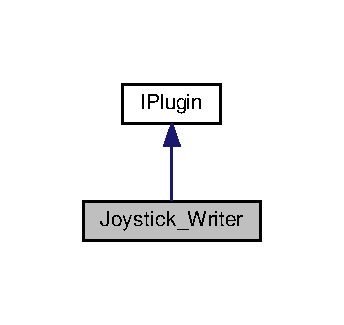
\includegraphics[width=165pt]{class_joystick___writer__inherit__graph}
\end{center}
\end{figure}


Collaboration diagram for Joystick\+\_\+\+Writer\+:\nopagebreak
\begin{figure}[H]
\begin{center}
\leavevmode
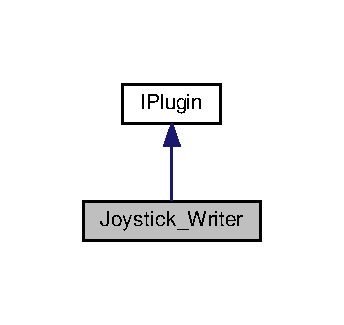
\includegraphics[width=165pt]{class_joystick___writer__coll__graph}
\end{center}
\end{figure}
\subsection*{Public Member Functions}
\begin{DoxyCompactItemize}
\item 
void \hyperlink{class_joystick___writer_aeb9c03f2389a5ed060b9c2a46fb84316}{Main} ()
\begin{DoxyCompactList}\small\item\em Main funcction of the plugin. \end{DoxyCompactList}\item 
bool \hyperlink{class_joystick___writer_a8c8c94397bbbb2058685ad6e0f92b4b1}{load\+Configuration} ()
\begin{DoxyCompactList}\small\item\em Load configuration. \end{DoxyCompactList}\item 
bool \hyperlink{class_joystick___writer_a67a56e0ae63ad59657f4745dcac2f7a3}{save\+Configuration} ()
\begin{DoxyCompactList}\small\item\em Save configuration. \end{DoxyCompactList}\item 
bool \hyperlink{class_joystick___writer_a3b341bb82658ee52172b22d90a18628f}{Initialize\+\_\+\+Output} ()
\begin{DoxyCompactList}\small\item\em Initialize Output variables for the plugin to publish. \end{DoxyCompactList}\item 
bool \hyperlink{class_joystick___writer_a4f7355cdbd819e5ce41575e152c98660}{Initialize\+\_\+\+Input} ()
\begin{DoxyCompactList}\small\item\em Initialize Input variables for the plugin to publish. \end{DoxyCompactList}\item 
\mbox{\Hypertarget{class_joystick___writer_a4bf2e08d435de90408c97e32dce88c45}\label{class_joystick___writer_a4bf2e08d435de90408c97e32dce88c45}} 
void {\bfseries Init\+\_\+\+Joy} ()
\item 
void \hyperlink{class_joystick___writer_aa1ab2778180c281887758883622b78bf}{run} ()
\begin{DoxyCompactList}\small\item\em Execute plugin. \end{DoxyCompactList}\item 
void \hyperlink{class_joystick___writer_a3c606f3961eea4b6a371146479ca26da}{stop} ()
\begin{DoxyCompactList}\small\item\em Stop plugin. \end{DoxyCompactList}\end{DoxyCompactItemize}
\subsection*{Additional Inherited Members}


\subsection{Detailed Description}
\hyperlink{class_joystick___writer}{Joystick\+\_\+\+Writer} plugin. 

This plugin is a legacy wrapper that alows us to use Hocoma\textquotesingle{}s games with this architecture it writes output to a shared memory segment defined by hocoma that can not be changed \begin{DoxyAuthor}{Author}
Patrick Heyer, \href{mailto:patrickhey@prodigy.net.mx}{\tt patrickhey@prodigy.\+net.\+mx} 
\end{DoxyAuthor}
\begin{DoxyDate}{Date}
jul 13, 2014 
\end{DoxyDate}
\begin{DoxyVersion}{Version}
1.\+0 
\end{DoxyVersion}


Definition at line 15 of file Joystick\+\_\+\+Writer.\+h.



\subsection{Member Function Documentation}
\mbox{\Hypertarget{class_joystick___writer_a4f7355cdbd819e5ce41575e152c98660}\label{class_joystick___writer_a4f7355cdbd819e5ce41575e152c98660}} 
\index{Joystick\+\_\+\+Writer@{Joystick\+\_\+\+Writer}!Initialize\+\_\+\+Input@{Initialize\+\_\+\+Input}}
\index{Initialize\+\_\+\+Input@{Initialize\+\_\+\+Input}!Joystick\+\_\+\+Writer@{Joystick\+\_\+\+Writer}}
\subsubsection{\texorpdfstring{Initialize\+\_\+\+Input()}{Initialize\_Input()}}
{\footnotesize\ttfamily bool Joystick\+\_\+\+Writer\+::\+Initialize\+\_\+\+Input (\begin{DoxyParamCaption}{ }\end{DoxyParamCaption})\hspace{0.3cm}{\ttfamily [virtual]}}



Initialize Input variables for the plugin to publish. 

\begin{DoxyReturn}{Returns}
bool 
\end{DoxyReturn}


Implements \hyperlink{class_i_plugin_aa7c66743ad956d8ada57becee559af4d}{I\+Plugin}.



Definition at line 134 of file Main.\+cpp.


\begin{DoxyCode}
135 \{
136     X\_axis=Shared\_Memory::getInstance().Register\_Double\_Input(\textcolor{stringliteral}{"Tracker\_X"});
137     Y\_axis=Shared\_Memory::getInstance().Register\_Double\_Input(\textcolor{stringliteral}{"Tracker\_Y"});
138     Z\_axis=Shared\_Memory::getInstance().Register\_Double\_Input(\textcolor{stringliteral}{"Tracker\_Z"});
139     RX\_axis=Shared\_Memory::getInstance().Register\_Double\_Input(\textcolor{stringliteral}{"Position\_For\_Game\_RX"});
140     RY\_axis=Shared\_Memory::getInstance().Register\_Double\_Input(\textcolor{stringliteral}{"Position\_For\_Game\_RY"});
141     RZ\_axis=Shared\_Memory::getInstance().Register\_Double\_Input(\textcolor{stringliteral}{"Position\_For\_Game\_RZ"});
142     \textcolor{keywordflow}{return} \textcolor{keyword}{true};
143 \}
\end{DoxyCode}
\mbox{\Hypertarget{class_joystick___writer_a3b341bb82658ee52172b22d90a18628f}\label{class_joystick___writer_a3b341bb82658ee52172b22d90a18628f}} 
\index{Joystick\+\_\+\+Writer@{Joystick\+\_\+\+Writer}!Initialize\+\_\+\+Output@{Initialize\+\_\+\+Output}}
\index{Initialize\+\_\+\+Output@{Initialize\+\_\+\+Output}!Joystick\+\_\+\+Writer@{Joystick\+\_\+\+Writer}}
\subsubsection{\texorpdfstring{Initialize\+\_\+\+Output()}{Initialize\_Output()}}
{\footnotesize\ttfamily bool Joystick\+\_\+\+Writer\+::\+Initialize\+\_\+\+Output (\begin{DoxyParamCaption}{ }\end{DoxyParamCaption})\hspace{0.3cm}{\ttfamily [virtual]}}



Initialize Output variables for the plugin to publish. 

\begin{DoxyReturn}{Returns}
bool 
\end{DoxyReturn}


Implements \hyperlink{class_i_plugin_a0b772513fc8c4ed01240e19c4bb84068}{I\+Plugin}.



Definition at line 129 of file Main.\+cpp.


\begin{DoxyCode}
130 \{
131     \textcolor{keywordflow}{return} \textcolor{keyword}{true};
132 \}
\end{DoxyCode}
\mbox{\Hypertarget{class_joystick___writer_a8c8c94397bbbb2058685ad6e0f92b4b1}\label{class_joystick___writer_a8c8c94397bbbb2058685ad6e0f92b4b1}} 
\index{Joystick\+\_\+\+Writer@{Joystick\+\_\+\+Writer}!load\+Configuration@{load\+Configuration}}
\index{load\+Configuration@{load\+Configuration}!Joystick\+\_\+\+Writer@{Joystick\+\_\+\+Writer}}
\subsubsection{\texorpdfstring{load\+Configuration()}{loadConfiguration()}}
{\footnotesize\ttfamily bool Joystick\+\_\+\+Writer\+::load\+Configuration (\begin{DoxyParamCaption}{ }\end{DoxyParamCaption})\hspace{0.3cm}{\ttfamily [virtual]}}



Load configuration. 

The configuration can be loaded from file, or be hard coded into the plugin (not recomended), initialization of public and private variables should occur here

By default load\+Configuration is called during \hyperlink{class_plugin_manager_a956e653b7db36da9d034b4a93c8308d5}{Plugin\+Manager\+::\+Initialize()} by the plugin manager.

\begin{DoxyReturn}{Returns}
bool 
\end{DoxyReturn}


Implements \hyperlink{class_i_plugin_a418cff309436d3a15d9a4ce7369db6dd}{I\+Plugin}.



Definition at line 119 of file Main.\+cpp.


\begin{DoxyCode}
120 \{
121     \textcolor{keywordflow}{return} \textcolor{keyword}{true};
122 \}
\end{DoxyCode}
\mbox{\Hypertarget{class_joystick___writer_aeb9c03f2389a5ed060b9c2a46fb84316}\label{class_joystick___writer_aeb9c03f2389a5ed060b9c2a46fb84316}} 
\index{Joystick\+\_\+\+Writer@{Joystick\+\_\+\+Writer}!Main@{Main}}
\index{Main@{Main}!Joystick\+\_\+\+Writer@{Joystick\+\_\+\+Writer}}
\subsubsection{\texorpdfstring{Main()}{Main()}}
{\footnotesize\ttfamily void Joystick\+\_\+\+Writer\+::\+Main (\begin{DoxyParamCaption}{ }\end{DoxyParamCaption})\hspace{0.3cm}{\ttfamily [virtual]}}



Main funcction of the plugin. 

Started in a new thread by the Run() funcction is the most importatn funcction of the plugin. Infinite loop (generaly a while(running) function that runs undefenitly in a read/process/write cicle). \begin{DoxyReturn}{Returns}
void 
\end{DoxyReturn}


Implements \hyperlink{class_i_plugin_ab5fdb3b0f7afdcee04324dca01766749}{I\+Plugin}.



Definition at line 57 of file Main.\+cpp.



References stop().


\begin{DoxyCode}
58 \{
59     \textcolor{keyword}{struct }uinput\_user\_dev uidev;
60 
61     \textcolor{keywordtype}{int}                    i;
62     \textcolor{keywordtype}{int}                    fd;
63 
64     fd = open(\textcolor{stringliteral}{"/dev/uinput"}, O\_WRONLY | O\_NONBLOCK);
65     \textcolor{keywordflow}{if}(fd < 0)
66         die(\textcolor{stringliteral}{"error: open"});
67 
68     memset(&uidev, 0, \textcolor{keyword}{sizeof}(uidev));
69     snprintf(uidev.name, UINPUT\_MAX\_NAME\_SIZE, \textcolor{stringliteral}{"Virtual\_joystick"});
70     uidev.id.bustype = BUS\_USB;
71     uidev.id.vendor  = 0x1;
72     uidev.id.product = 0x1;
73     uidev.id.version = 1;
74 
75     ioctl (fd, UI\_SET\_EVBIT, EV\_SYN);
76     ioctl (fd, UI\_SET\_EVBIT, EV\_ABS);
77     ioctl (fd, UI\_SET\_EVBIT, EV\_KEY);
78 
79     ioctl (fd, UI\_SET\_ABSBIT, ABS\_X);
80     ioctl (fd, UI\_SET\_ABSBIT, ABS\_Y);
81     ioctl (fd, UI\_SET\_ABSBIT, ABS\_Z);
82     ioctl (fd, UI\_SET\_ABSBIT, ABS\_RX);
83     ioctl (fd, UI\_SET\_ABSBIT, ABS\_RY);
84     ioctl (fd, UI\_SET\_ABSBIT, ABS\_RZ);
85     ioctl (fd, UI\_SET\_ABSBIT, ABS\_RT);
86     ioctl (fd, UI\_SET\_ABSBIT, ABS\_MAX);
87 
88     \textcolor{keywordflow}{for}(i = 0; i < ABS\_MAX; ++i)
89     \{
90         uidev.absmax[i] = 511;
91         uidev.absmin[i] = -512;
92     \}
93 
94     \textcolor{comment}{// Create device}
95     write (fd, &uidev, \textcolor{keyword}{sizeof} (uidev));
96     \textcolor{keywordflow}{if} (ioctl (fd, UI\_DEV\_CREATE))
97     \{
98         LOG(WARNING) << \textcolor{stringliteral}{"Unable to create UIDEVUT device."};
99         LOG(ERROR) << PluginDisplayName << \textcolor{stringliteral}{" will NOT keep executing"};
100         \hyperlink{class_joystick___writer_a3c606f3961eea4b6a371146479ca26da}{stop}();
101     running=\textcolor{keyword}{false};
102     stoped = \textcolor{keyword}{true};
103     \textcolor{keywordflow}{return};
104     \}
105 
106     \textcolor{keywordflow}{while}(running)
107     \{
108         do\_uinput(fd,ABS\_X,*X\_axis*32767, EV\_ABS);
109         do\_uinput(fd,ABS\_Y,*Y\_axis*32767, EV\_ABS);
110         do\_uinput(fd,ABS\_Z,*Z\_axis*32767, EV\_ABS);
111         do\_uinput(fd,ABS\_RX,*RX\_axis*32767, EV\_ABS);
112         do\_uinput(fd,ABS\_RY,*RY\_axis*32767, EV\_ABS);
113         do\_uinput(fd,ABS\_RZ,*RZ\_axis*32767, EV\_ABS);
114     \}
115     stoped = \textcolor{keyword}{true};
116     \textcolor{keywordflow}{return};
117 \}
\end{DoxyCode}
\mbox{\Hypertarget{class_joystick___writer_aa1ab2778180c281887758883622b78bf}\label{class_joystick___writer_aa1ab2778180c281887758883622b78bf}} 
\index{Joystick\+\_\+\+Writer@{Joystick\+\_\+\+Writer}!run@{run}}
\index{run@{run}!Joystick\+\_\+\+Writer@{Joystick\+\_\+\+Writer}}
\subsubsection{\texorpdfstring{run()}{run()}}
{\footnotesize\ttfamily void Joystick\+\_\+\+Writer\+::run (\begin{DoxyParamCaption}{ }\end{DoxyParamCaption})\hspace{0.3cm}{\ttfamily [virtual]}}



Execute plugin. 

Starts a new thread and executes the plugins main() funcction. \begin{DoxyReturn}{Returns}
void 
\end{DoxyReturn}


Implements \hyperlink{class_i_plugin_a46b4ace767e77f9db9c9585e99c09039}{I\+Plugin}.



Definition at line 145 of file Main.\+cpp.



References I\+Plugin\+::\+Inc\+Wrapper().


\begin{DoxyCode}
146 \{
147     pthread\_create(&thread\_id, NULL, &\hyperlink{class_i_plugin_a62d22be2fdf66eb7f5c2f797f5f3d7f3}{IPlugin::IncWrapper}, \textcolor{keyword}{this});
148     running = \textcolor{keyword}{true};
149     stoped = \textcolor{keyword}{false};
150 \}
\end{DoxyCode}
\mbox{\Hypertarget{class_joystick___writer_a67a56e0ae63ad59657f4745dcac2f7a3}\label{class_joystick___writer_a67a56e0ae63ad59657f4745dcac2f7a3}} 
\index{Joystick\+\_\+\+Writer@{Joystick\+\_\+\+Writer}!save\+Configuration@{save\+Configuration}}
\index{save\+Configuration@{save\+Configuration}!Joystick\+\_\+\+Writer@{Joystick\+\_\+\+Writer}}
\subsubsection{\texorpdfstring{save\+Configuration()}{saveConfiguration()}}
{\footnotesize\ttfamily bool Joystick\+\_\+\+Writer\+::save\+Configuration (\begin{DoxyParamCaption}{ }\end{DoxyParamCaption})\hspace{0.3cm}{\ttfamily [virtual]}}



Save configuration. 

The configuration should be saved to file, public and private variables that should be configured at startup should be saved.

By default save\+Configuration is called during \hyperlink{class_plugin_manager_ab651a05d6fcb92562807e9f5ecc30855}{Plugin\+Manager\+::\+Unload()} by the plugin manager.

\begin{DoxyReturn}{Returns}
bool 
\end{DoxyReturn}


Implements \hyperlink{class_i_plugin_a79b5c42b1c7b08257a6110b2091039bc}{I\+Plugin}.



Definition at line 124 of file Main.\+cpp.


\begin{DoxyCode}
125 \{
126     \textcolor{keywordflow}{return} \textcolor{keyword}{true};
127 \}
\end{DoxyCode}
\mbox{\Hypertarget{class_joystick___writer_a3c606f3961eea4b6a371146479ca26da}\label{class_joystick___writer_a3c606f3961eea4b6a371146479ca26da}} 
\index{Joystick\+\_\+\+Writer@{Joystick\+\_\+\+Writer}!stop@{stop}}
\index{stop@{stop}!Joystick\+\_\+\+Writer@{Joystick\+\_\+\+Writer}}
\subsubsection{\texorpdfstring{stop()}{stop()}}
{\footnotesize\ttfamily void Joystick\+\_\+\+Writer\+::stop (\begin{DoxyParamCaption}{ }\end{DoxyParamCaption})\hspace{0.3cm}{\ttfamily [virtual]}}



Stop plugin. 

Stops the plugin \begin{DoxyReturn}{Returns}
void 
\end{DoxyReturn}


Implements \hyperlink{class_i_plugin_a86e523c283aec5c9fb21249a76e916ac}{I\+Plugin}.



Definition at line 153 of file Main.\+cpp.



Referenced by Main().


\begin{DoxyCode}
154 \{
155     running = \textcolor{keyword}{false};
156 \}
\end{DoxyCode}


The documentation for this class was generated from the following files\+:\begin{DoxyCompactItemize}
\item 
/home/patrick/projects/\+Gesture\+\_\+\+Therapy\+\_\+\+Linux/src/\+Joystick\+\_\+\+Writer/Joystick\+\_\+\+Writer.\+h\item 
/home/patrick/projects/\+Gesture\+\_\+\+Therapy\+\_\+\+Linux/src/\+Joystick\+\_\+\+Writer/Main.\+cpp\end{DoxyCompactItemize}

\hypertarget{struct_config_file_1_1key__not__found}{}\section{Config\+File\+:\+:key\+\_\+not\+\_\+found Struct Reference}
\label{struct_config_file_1_1key__not__found}\index{Config\+File\+::key\+\_\+not\+\_\+found@{Config\+File\+::key\+\_\+not\+\_\+found}}


Collaboration diagram for Config\+File\+:\+:key\+\_\+not\+\_\+found\+:\nopagebreak
\begin{figure}[H]
\begin{center}
\leavevmode
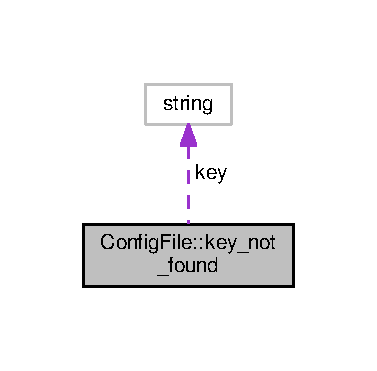
\includegraphics[width=181pt]{struct_config_file_1_1key__not__found__coll__graph}
\end{center}
\end{figure}
\subsection*{Public Member Functions}
\begin{DoxyCompactItemize}
\item 
\mbox{\Hypertarget{struct_config_file_1_1key__not__found_aedacf2df70a4aa179448706b4862d768}\label{struct_config_file_1_1key__not__found_aedacf2df70a4aa179448706b4862d768}} 
{\bfseries key\+\_\+not\+\_\+found} (const string \&key\+\_\+=string())
\end{DoxyCompactItemize}
\subsection*{Public Attributes}
\begin{DoxyCompactItemize}
\item 
\mbox{\Hypertarget{struct_config_file_1_1key__not__found_a2872cbeb5ab860f357b3a58dd867b90b}\label{struct_config_file_1_1key__not__found_a2872cbeb5ab860f357b3a58dd867b90b}} 
string {\bfseries key}
\end{DoxyCompactItemize}


\subsection{Detailed Description}


Definition at line 112 of file Config\+File.\+h.



The documentation for this struct was generated from the following file\+:\begin{DoxyCompactItemize}
\item 
/home/patrick/projects/\+Gesture\+\_\+\+Therapy\+\_\+\+Linux/src/include/Config\+File.\+h\end{DoxyCompactItemize}

\hypertarget{class_network___client}{}\section{Network\+\_\+\+Client Class Reference}
\label{class_network___client}\index{Network\+\_\+\+Client@{Network\+\_\+\+Client}}


\hyperlink{class_network___client}{Network\+\_\+\+Client} plugin.  




Inheritance diagram for Network\+\_\+\+Client\+:\nopagebreak
\begin{figure}[H]
\begin{center}
\leavevmode
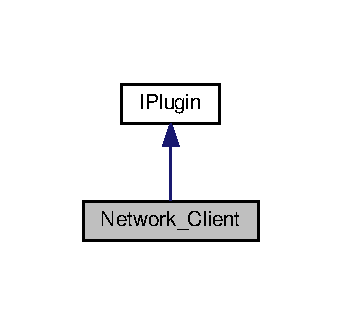
\includegraphics[width=164pt]{class_network___client__inherit__graph}
\end{center}
\end{figure}


Collaboration diagram for Network\+\_\+\+Client\+:\nopagebreak
\begin{figure}[H]
\begin{center}
\leavevmode
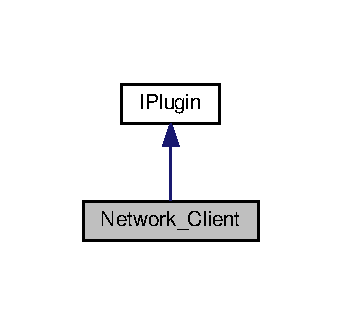
\includegraphics[width=164pt]{class_network___client__coll__graph}
\end{center}
\end{figure}
\subsection*{Public Member Functions}
\begin{DoxyCompactItemize}
\item 
void \hyperlink{class_network___client_a711e61f7233983449a1f4a50a4009b87}{Main} ()
\begin{DoxyCompactList}\small\item\em Main funcction of the plugin. \end{DoxyCompactList}\item 
bool \hyperlink{class_network___client_a02e30223901e61514ee59eccec70dddf}{load\+Configuration} ()
\begin{DoxyCompactList}\small\item\em Load configuration. \end{DoxyCompactList}\item 
bool \hyperlink{class_network___client_aeaa8dcaafdecc5a9f417dc07060d6261}{save\+Configuration} ()
\begin{DoxyCompactList}\small\item\em Save configuration. \end{DoxyCompactList}\item 
bool \hyperlink{class_network___client_ae7279167c7343c8a8304f55a5f24c802}{Initialize\+\_\+\+Output} ()
\begin{DoxyCompactList}\small\item\em Initialize Output variables for the plugin to publish. \end{DoxyCompactList}\item 
bool \hyperlink{class_network___client_a429b34311701bc58b617c7e0675e70fa}{Initialize\+\_\+\+Input} ()
\begin{DoxyCompactList}\small\item\em Initialize Input variables for the plugin to publish. \end{DoxyCompactList}\item 
void \hyperlink{class_network___client_a8831a63a0892de0f975e61b3d68473c7}{run} ()
\begin{DoxyCompactList}\small\item\em Execute plugin. \end{DoxyCompactList}\item 
void \hyperlink{class_network___client_ad54dbc2ec20d9fbabcb5265401d072c2}{stop} ()
\begin{DoxyCompactList}\small\item\em Stop plugin. \end{DoxyCompactList}\end{DoxyCompactItemize}
\subsection*{Additional Inherited Members}


\subsection{Detailed Description}
\hyperlink{class_network___client}{Network\+\_\+\+Client} plugin. 

This plugin is a network server that accepts client conections to comunicate with other programs (running on the same computer or over the network) \begin{DoxyAuthor}{Author}
Patrick Heyer, \href{mailto:patrickhey@prodigy.net.mx}{\tt patrickhey@prodigy.\+net.\+mx}, Juan Herrera \href{mailto:juan_antonio_@hotmail.com}{\tt juan\+\_\+antonio\+\_\+@hotmail.\+com}, Manuel Oropeza \href{mailto:zodiacanimations@msn.com}{\tt zodiacanimations@msn.\+com} 
\end{DoxyAuthor}
\begin{DoxyDate}{Date}
jul 04, 2012 
\end{DoxyDate}
\begin{DoxyVersion}{Version}
1.\+0 
\end{DoxyVersion}


Definition at line 33 of file Main.\+cpp.



\subsection{Member Function Documentation}
\mbox{\Hypertarget{class_network___client_a429b34311701bc58b617c7e0675e70fa}\label{class_network___client_a429b34311701bc58b617c7e0675e70fa}} 
\index{Network\+\_\+\+Client@{Network\+\_\+\+Client}!Initialize\+\_\+\+Input@{Initialize\+\_\+\+Input}}
\index{Initialize\+\_\+\+Input@{Initialize\+\_\+\+Input}!Network\+\_\+\+Client@{Network\+\_\+\+Client}}
\subsubsection{\texorpdfstring{Initialize\+\_\+\+Input()}{Initialize\_Input()}}
{\footnotesize\ttfamily bool Network\+\_\+\+Client\+::\+Initialize\+\_\+\+Input (\begin{DoxyParamCaption}{ }\end{DoxyParamCaption})\hspace{0.3cm}{\ttfamily [virtual]}}



Initialize Input variables for the plugin to publish. 

\begin{DoxyReturn}{Returns}
bool 
\end{DoxyReturn}


Implements \hyperlink{class_i_plugin_aa7c66743ad956d8ada57becee559af4d}{I\+Plugin}.



Definition at line 106 of file Main.\+cpp.


\begin{DoxyCode}
107 \{
108     \textcolor{keywordflow}{return} \textcolor{keyword}{true};
109 \}
\end{DoxyCode}
\mbox{\Hypertarget{class_network___client_ae7279167c7343c8a8304f55a5f24c802}\label{class_network___client_ae7279167c7343c8a8304f55a5f24c802}} 
\index{Network\+\_\+\+Client@{Network\+\_\+\+Client}!Initialize\+\_\+\+Output@{Initialize\+\_\+\+Output}}
\index{Initialize\+\_\+\+Output@{Initialize\+\_\+\+Output}!Network\+\_\+\+Client@{Network\+\_\+\+Client}}
\subsubsection{\texorpdfstring{Initialize\+\_\+\+Output()}{Initialize\_Output()}}
{\footnotesize\ttfamily bool Network\+\_\+\+Client\+::\+Initialize\+\_\+\+Output (\begin{DoxyParamCaption}{ }\end{DoxyParamCaption})\hspace{0.3cm}{\ttfamily [virtual]}}



Initialize Output variables for the plugin to publish. 

\begin{DoxyReturn}{Returns}
bool 
\end{DoxyReturn}


Implements \hyperlink{class_i_plugin_a0b772513fc8c4ed01240e19c4bb84068}{I\+Plugin}.



Definition at line 100 of file Main.\+cpp.


\begin{DoxyCode}
101 \{
102 
103     \textcolor{keywordflow}{return} \textcolor{keyword}{true};
104 \}
\end{DoxyCode}
\mbox{\Hypertarget{class_network___client_a02e30223901e61514ee59eccec70dddf}\label{class_network___client_a02e30223901e61514ee59eccec70dddf}} 
\index{Network\+\_\+\+Client@{Network\+\_\+\+Client}!load\+Configuration@{load\+Configuration}}
\index{load\+Configuration@{load\+Configuration}!Network\+\_\+\+Client@{Network\+\_\+\+Client}}
\subsubsection{\texorpdfstring{load\+Configuration()}{loadConfiguration()}}
{\footnotesize\ttfamily bool Network\+\_\+\+Client\+::load\+Configuration (\begin{DoxyParamCaption}{ }\end{DoxyParamCaption})\hspace{0.3cm}{\ttfamily [virtual]}}



Load configuration. 

The configuration can be loaded from file, or be hard coded into the plugin (not recomended), initialization of public and private variables should occur here

By default load\+Configuration is called during \hyperlink{class_plugin_manager_a956e653b7db36da9d034b4a93c8308d5}{Plugin\+Manager\+::\+Initialize()} by the plugin manager.

\begin{DoxyReturn}{Returns}
bool 
\end{DoxyReturn}


Implements \hyperlink{class_i_plugin_a418cff309436d3a15d9a4ce7369db6dd}{I\+Plugin}.



Definition at line 90 of file Main.\+cpp.


\begin{DoxyCode}
91 \{
92     \textcolor{keywordflow}{return} \textcolor{keyword}{true};
93 \}
\end{DoxyCode}
\mbox{\Hypertarget{class_network___client_a711e61f7233983449a1f4a50a4009b87}\label{class_network___client_a711e61f7233983449a1f4a50a4009b87}} 
\index{Network\+\_\+\+Client@{Network\+\_\+\+Client}!Main@{Main}}
\index{Main@{Main}!Network\+\_\+\+Client@{Network\+\_\+\+Client}}
\subsubsection{\texorpdfstring{Main()}{Main()}}
{\footnotesize\ttfamily void Network\+\_\+\+Client\+::\+Main (\begin{DoxyParamCaption}{ }\end{DoxyParamCaption})\hspace{0.3cm}{\ttfamily [virtual]}}



Main funcction of the plugin. 

Started in a new thread by the Run() funcction is the most importatn funcction of the plugin. Infinite loop (generaly a while(running) function that runs undefenitly in a read/process/write cicle). \begin{DoxyReturn}{Returns}
void 
\end{DoxyReturn}


Implements \hyperlink{class_i_plugin_ab5fdb3b0f7afdcee04324dca01766749}{I\+Plugin}.



Definition at line 67 of file Main.\+cpp.


\begin{DoxyCode}
68 \{
69     sleep(5);
70     NetThread *net = \textcolor{keyword}{new}  NetThread();
71     net->SetOutputStream(stdout);
72     net->OpenOutputAddress(\textcolor{stringliteral}{"localhost"}, 2070);
73     net->Write(\textcolor{stringliteral}{"send"});
74     \textcolor{keywordflow}{while}(running)
75     \{
76         net->Read();
77         \textcolor{keywordflow}{if}(net->GetStatus()>0)
78         \{
79             \textcolor{keywordtype}{string} s = net->GetIncoming();
80             \textcolor{keywordflow}{if} (s.find(\textcolor{stringliteral}{"recived"})!=s.npos)
81             \{
82                 net->messages.clear();
83                 net->Write(\textcolor{stringliteral}{"send"});
84             \}
85         \}
86     \}
87     stoped=\textcolor{keyword}{true};
88 \}
\end{DoxyCode}
\mbox{\Hypertarget{class_network___client_a8831a63a0892de0f975e61b3d68473c7}\label{class_network___client_a8831a63a0892de0f975e61b3d68473c7}} 
\index{Network\+\_\+\+Client@{Network\+\_\+\+Client}!run@{run}}
\index{run@{run}!Network\+\_\+\+Client@{Network\+\_\+\+Client}}
\subsubsection{\texorpdfstring{run()}{run()}}
{\footnotesize\ttfamily void Network\+\_\+\+Client\+::run (\begin{DoxyParamCaption}{ }\end{DoxyParamCaption})\hspace{0.3cm}{\ttfamily [virtual]}}



Execute plugin. 

Starts a new thread and executes the plugins main() funcction. \begin{DoxyReturn}{Returns}
void 
\end{DoxyReturn}


Implements \hyperlink{class_i_plugin_a46b4ace767e77f9db9c9585e99c09039}{I\+Plugin}.



Definition at line 111 of file Main.\+cpp.



References I\+Plugin\+::\+Inc\+Wrapper().


\begin{DoxyCode}
112 \{
113     pthread\_create(&thread\_id, NULL, &\hyperlink{class_i_plugin_a62d22be2fdf66eb7f5c2f797f5f3d7f3}{IPlugin::IncWrapper}, \textcolor{keyword}{this});
114     running = \textcolor{keyword}{true};
115     stoped = \textcolor{keyword}{false};
116 \}
\end{DoxyCode}
\mbox{\Hypertarget{class_network___client_aeaa8dcaafdecc5a9f417dc07060d6261}\label{class_network___client_aeaa8dcaafdecc5a9f417dc07060d6261}} 
\index{Network\+\_\+\+Client@{Network\+\_\+\+Client}!save\+Configuration@{save\+Configuration}}
\index{save\+Configuration@{save\+Configuration}!Network\+\_\+\+Client@{Network\+\_\+\+Client}}
\subsubsection{\texorpdfstring{save\+Configuration()}{saveConfiguration()}}
{\footnotesize\ttfamily bool Network\+\_\+\+Client\+::save\+Configuration (\begin{DoxyParamCaption}{ }\end{DoxyParamCaption})\hspace{0.3cm}{\ttfamily [virtual]}}



Save configuration. 

The configuration should be saved to file, public and private variables that should be configured at startup should be saved.

By default save\+Configuration is called during \hyperlink{class_plugin_manager_ab651a05d6fcb92562807e9f5ecc30855}{Plugin\+Manager\+::\+Unload()} by the plugin manager.

\begin{DoxyReturn}{Returns}
bool 
\end{DoxyReturn}


Implements \hyperlink{class_i_plugin_a79b5c42b1c7b08257a6110b2091039bc}{I\+Plugin}.



Definition at line 95 of file Main.\+cpp.


\begin{DoxyCode}
96 \{
97     \textcolor{keywordflow}{return} \textcolor{keyword}{true};
98 \}
\end{DoxyCode}
\mbox{\Hypertarget{class_network___client_ad54dbc2ec20d9fbabcb5265401d072c2}\label{class_network___client_ad54dbc2ec20d9fbabcb5265401d072c2}} 
\index{Network\+\_\+\+Client@{Network\+\_\+\+Client}!stop@{stop}}
\index{stop@{stop}!Network\+\_\+\+Client@{Network\+\_\+\+Client}}
\subsubsection{\texorpdfstring{stop()}{stop()}}
{\footnotesize\ttfamily void Network\+\_\+\+Client\+::stop (\begin{DoxyParamCaption}{ }\end{DoxyParamCaption})\hspace{0.3cm}{\ttfamily [virtual]}}



Stop plugin. 

Stops the plugin \begin{DoxyReturn}{Returns}
void 
\end{DoxyReturn}


Implements \hyperlink{class_i_plugin_a86e523c283aec5c9fb21249a76e916ac}{I\+Plugin}.



Definition at line 118 of file Main.\+cpp.


\begin{DoxyCode}
119 \{
120     running = \textcolor{keyword}{false};
121 \}
\end{DoxyCode}


The documentation for this class was generated from the following file\+:\begin{DoxyCompactItemize}
\item 
/home/patrick/projects/\+Gesture\+\_\+\+Therapy\+\_\+\+Linux/src/\+Network\+\_\+\+Client/Main.\+cpp\end{DoxyCompactItemize}

\hypertarget{class_network___server}{}\section{Network\+\_\+\+Server Class Reference}
\label{class_network___server}\index{Network\+\_\+\+Server@{Network\+\_\+\+Server}}


\hyperlink{class_network___server}{Network\+\_\+\+Server} plugin.  




Inheritance diagram for Network\+\_\+\+Server\+:\nopagebreak
\begin{figure}[H]
\begin{center}
\leavevmode
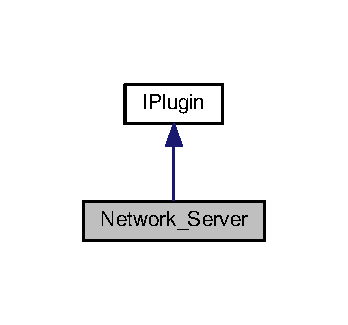
\includegraphics[width=167pt]{class_network___server__inherit__graph}
\end{center}
\end{figure}


Collaboration diagram for Network\+\_\+\+Server\+:\nopagebreak
\begin{figure}[H]
\begin{center}
\leavevmode
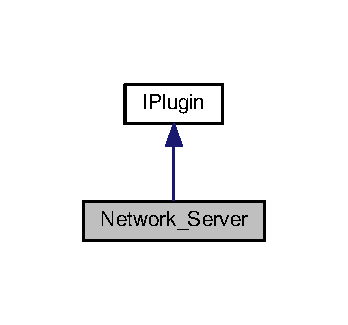
\includegraphics[width=167pt]{class_network___server__coll__graph}
\end{center}
\end{figure}
\subsection*{Public Member Functions}
\begin{DoxyCompactItemize}
\item 
void \hyperlink{class_network___server_aa9d6cd53b5c62355518ad0a32ba1444b}{Main} ()
\begin{DoxyCompactList}\small\item\em Main funcction of the plugin. \end{DoxyCompactList}\item 
bool \hyperlink{class_network___server_a60edfbf13d3812f66381dca40fbe0801}{load\+Configuration} ()
\begin{DoxyCompactList}\small\item\em Load configuration. \end{DoxyCompactList}\item 
bool \hyperlink{class_network___server_a859ab976d5a6f1761f49e3e7abc6bb73}{save\+Configuration} ()
\begin{DoxyCompactList}\small\item\em Save configuration. \end{DoxyCompactList}\item 
bool \hyperlink{class_network___server_a9ddcc321be18d2a6c28f51a3b94983ff}{Initialize\+\_\+\+Output} ()
\begin{DoxyCompactList}\small\item\em Initialize Output variables for the plugin to publish. \end{DoxyCompactList}\item 
bool \hyperlink{class_network___server_ad5129bb2f3bcf2480a33a42a36cd5352}{Initialize\+\_\+\+Input} ()
\begin{DoxyCompactList}\small\item\em Initialize Input variables for the plugin to publish. \end{DoxyCompactList}\item 
void \hyperlink{class_network___server_ac8778efb5b94041cafa3e57d57e8d9a2}{run} ()
\begin{DoxyCompactList}\small\item\em Execute plugin. \end{DoxyCompactList}\item 
void \hyperlink{class_network___server_a9a4400df0ce8da4c24c8758201b68562}{stop} ()
\begin{DoxyCompactList}\small\item\em Stop plugin. \end{DoxyCompactList}\end{DoxyCompactItemize}
\subsection*{Additional Inherited Members}


\subsection{Detailed Description}
\hyperlink{class_network___server}{Network\+\_\+\+Server} plugin. 

This plugin is a network server that accepts client conections to comunicate with other programs (running on the same computer or over the network) \begin{DoxyAuthor}{Author}
Patrick Heyer, \href{mailto:patrickhey@prodigy.net.mx}{\tt patrickhey@prodigy.\+net.\+mx}, Juan Herrera \href{mailto:juan_antonio_@hotmail.com}{\tt juan\+\_\+antonio\+\_\+@hotmail.\+com}, Manuel Oropeza \href{mailto:zodiacanimations@msn.com}{\tt zodiacanimations@msn.\+com} 
\end{DoxyAuthor}
\begin{DoxyDate}{Date}
jul 04, 2012 
\end{DoxyDate}
\begin{DoxyVersion}{Version}
1.\+0 
\end{DoxyVersion}


Definition at line 35 of file Main.\+cpp.



\subsection{Member Function Documentation}
\mbox{\Hypertarget{class_network___server_ad5129bb2f3bcf2480a33a42a36cd5352}\label{class_network___server_ad5129bb2f3bcf2480a33a42a36cd5352}} 
\index{Network\+\_\+\+Server@{Network\+\_\+\+Server}!Initialize\+\_\+\+Input@{Initialize\+\_\+\+Input}}
\index{Initialize\+\_\+\+Input@{Initialize\+\_\+\+Input}!Network\+\_\+\+Server@{Network\+\_\+\+Server}}
\subsubsection{\texorpdfstring{Initialize\+\_\+\+Input()}{Initialize\_Input()}}
{\footnotesize\ttfamily bool Network\+\_\+\+Server\+::\+Initialize\+\_\+\+Input (\begin{DoxyParamCaption}{ }\end{DoxyParamCaption})\hspace{0.3cm}{\ttfamily [virtual]}}



Initialize Input variables for the plugin to publish. 

\begin{DoxyReturn}{Returns}
bool 
\end{DoxyReturn}


Implements \hyperlink{class_i_plugin_aa7c66743ad956d8ada57becee559af4d}{I\+Plugin}.



Definition at line 132 of file Main.\+cpp.


\begin{DoxyCode}
133 \{
134     \textcolor{keywordflow}{return} \textcolor{keyword}{true};
135 \}
\end{DoxyCode}
\mbox{\Hypertarget{class_network___server_a9ddcc321be18d2a6c28f51a3b94983ff}\label{class_network___server_a9ddcc321be18d2a6c28f51a3b94983ff}} 
\index{Network\+\_\+\+Server@{Network\+\_\+\+Server}!Initialize\+\_\+\+Output@{Initialize\+\_\+\+Output}}
\index{Initialize\+\_\+\+Output@{Initialize\+\_\+\+Output}!Network\+\_\+\+Server@{Network\+\_\+\+Server}}
\subsubsection{\texorpdfstring{Initialize\+\_\+\+Output()}{Initialize\_Output()}}
{\footnotesize\ttfamily bool Network\+\_\+\+Server\+::\+Initialize\+\_\+\+Output (\begin{DoxyParamCaption}{ }\end{DoxyParamCaption})\hspace{0.3cm}{\ttfamily [virtual]}}



Initialize Output variables for the plugin to publish. 

\begin{DoxyReturn}{Returns}
bool 
\end{DoxyReturn}


Implements \hyperlink{class_i_plugin_a0b772513fc8c4ed01240e19c4bb84068}{I\+Plugin}.



Definition at line 126 of file Main.\+cpp.


\begin{DoxyCode}
127 \{
128     Shared\_Memory::getInstance().Register\_Output(\textcolor{stringliteral}{"Server\_Phrase"}, &phrase);
129     \textcolor{keywordflow}{return} \textcolor{keyword}{true};
130 \}
\end{DoxyCode}
\mbox{\Hypertarget{class_network___server_a60edfbf13d3812f66381dca40fbe0801}\label{class_network___server_a60edfbf13d3812f66381dca40fbe0801}} 
\index{Network\+\_\+\+Server@{Network\+\_\+\+Server}!load\+Configuration@{load\+Configuration}}
\index{load\+Configuration@{load\+Configuration}!Network\+\_\+\+Server@{Network\+\_\+\+Server}}
\subsubsection{\texorpdfstring{load\+Configuration()}{loadConfiguration()}}
{\footnotesize\ttfamily bool Network\+\_\+\+Server\+::load\+Configuration (\begin{DoxyParamCaption}{ }\end{DoxyParamCaption})\hspace{0.3cm}{\ttfamily [virtual]}}



Load configuration. 

The configuration can be loaded from file, or be hard coded into the plugin (not recomended), initialization of public and private variables should occur here

By default load\+Configuration is called during \hyperlink{class_plugin_manager_a956e653b7db36da9d034b4a93c8308d5}{Plugin\+Manager\+::\+Initialize()} by the plugin manager.

\begin{DoxyReturn}{Returns}
bool 
\end{DoxyReturn}


Implements \hyperlink{class_i_plugin_a418cff309436d3a15d9a4ce7369db6dd}{I\+Plugin}.



Definition at line 116 of file Main.\+cpp.


\begin{DoxyCode}
117 \{
118     \textcolor{keywordflow}{return} \textcolor{keyword}{true};
119 \}
\end{DoxyCode}
\mbox{\Hypertarget{class_network___server_aa9d6cd53b5c62355518ad0a32ba1444b}\label{class_network___server_aa9d6cd53b5c62355518ad0a32ba1444b}} 
\index{Network\+\_\+\+Server@{Network\+\_\+\+Server}!Main@{Main}}
\index{Main@{Main}!Network\+\_\+\+Server@{Network\+\_\+\+Server}}
\subsubsection{\texorpdfstring{Main()}{Main()}}
{\footnotesize\ttfamily void Network\+\_\+\+Server\+::\+Main (\begin{DoxyParamCaption}{ }\end{DoxyParamCaption})\hspace{0.3cm}{\ttfamily [virtual]}}



Main funcction of the plugin. 

Started in a new thread by the Run() funcction is the most importatn funcction of the plugin. Infinite loop (generaly a while(running) function that runs undefenitly in a read/process/write cicle). \begin{DoxyReturn}{Returns}
void 
\end{DoxyReturn}


Implements \hyperlink{class_i_plugin_ab5fdb3b0f7afdcee04324dca01766749}{I\+Plugin}.



Definition at line 73 of file Main.\+cpp.


\begin{DoxyCode}
74 \{
75     NetThread *net = \textcolor{keyword}{new} NetThread();
76     phrase=\textcolor{stringliteral}{" "};
77     net->SetOutputStream(stdout);
78     net->OpenReadPort(2070);
79     net->start();
80     net->Accept();
81 
82     std::string respuesta;
83     
84     \textcolor{keywordflow}{while}(running)
85     \{
86         net->Read();
87         \textcolor{keywordflow}{if}(net->GetStatus()>0)
88         \{
89             phrase = net->GetIncoming();
90             std::cout << \textcolor{stringliteral}{"client says "} << phrase << std::endl;
91             \textcolor{keywordflow}{if}(phrase==\textcolor{stringliteral}{"Connecting"})
92             \{
93                 net->messages.clear();
94                 net->Write(\textcolor{stringliteral}{"Connected"});
95             \}
96             \textcolor{keywordflow}{if}(phrase==\textcolor{stringliteral}{"next\_target"})
97             \{
98                 net->messages.clear();
99                 net->Write(\textcolor{stringliteral}{"Target\_Bed\_Upstairs"});
100                 std::cout << \textcolor{stringliteral}{"enviado a Target\_Bed\_Upstairs"} << std::endl;
101             \}
102         \}
103         \textcolor{keywordflow}{else}
104         \{
105             phrase=\textcolor{stringliteral}{" "};
106             
107         \}
108         usleep(500);
109         
110     \}
111     stoped=\textcolor{keyword}{true};
112 
113 \}
\end{DoxyCode}
\mbox{\Hypertarget{class_network___server_ac8778efb5b94041cafa3e57d57e8d9a2}\label{class_network___server_ac8778efb5b94041cafa3e57d57e8d9a2}} 
\index{Network\+\_\+\+Server@{Network\+\_\+\+Server}!run@{run}}
\index{run@{run}!Network\+\_\+\+Server@{Network\+\_\+\+Server}}
\subsubsection{\texorpdfstring{run()}{run()}}
{\footnotesize\ttfamily void Network\+\_\+\+Server\+::run (\begin{DoxyParamCaption}{ }\end{DoxyParamCaption})\hspace{0.3cm}{\ttfamily [virtual]}}



Execute plugin. 

Starts a new thread and executes the plugins main() funcction. \begin{DoxyReturn}{Returns}
void 
\end{DoxyReturn}


Implements \hyperlink{class_i_plugin_a46b4ace767e77f9db9c9585e99c09039}{I\+Plugin}.



Definition at line 137 of file Main.\+cpp.



References I\+Plugin\+::\+Inc\+Wrapper().


\begin{DoxyCode}
138 \{
139     pthread\_create(&thread\_id, NULL, &\hyperlink{class_i_plugin_a62d22be2fdf66eb7f5c2f797f5f3d7f3}{IPlugin::IncWrapper}, \textcolor{keyword}{this});
140     running = \textcolor{keyword}{true};
141     stoped = \textcolor{keyword}{false};
142 \}
\end{DoxyCode}
\mbox{\Hypertarget{class_network___server_a859ab976d5a6f1761f49e3e7abc6bb73}\label{class_network___server_a859ab976d5a6f1761f49e3e7abc6bb73}} 
\index{Network\+\_\+\+Server@{Network\+\_\+\+Server}!save\+Configuration@{save\+Configuration}}
\index{save\+Configuration@{save\+Configuration}!Network\+\_\+\+Server@{Network\+\_\+\+Server}}
\subsubsection{\texorpdfstring{save\+Configuration()}{saveConfiguration()}}
{\footnotesize\ttfamily bool Network\+\_\+\+Server\+::save\+Configuration (\begin{DoxyParamCaption}{ }\end{DoxyParamCaption})\hspace{0.3cm}{\ttfamily [virtual]}}



Save configuration. 

The configuration should be saved to file, public and private variables that should be configured at startup should be saved.

By default save\+Configuration is called during \hyperlink{class_plugin_manager_ab651a05d6fcb92562807e9f5ecc30855}{Plugin\+Manager\+::\+Unload()} by the plugin manager.

\begin{DoxyReturn}{Returns}
bool 
\end{DoxyReturn}


Implements \hyperlink{class_i_plugin_a79b5c42b1c7b08257a6110b2091039bc}{I\+Plugin}.



Definition at line 121 of file Main.\+cpp.


\begin{DoxyCode}
122 \{
123     \textcolor{keywordflow}{return} \textcolor{keyword}{true};
124 \}
\end{DoxyCode}
\mbox{\Hypertarget{class_network___server_a9a4400df0ce8da4c24c8758201b68562}\label{class_network___server_a9a4400df0ce8da4c24c8758201b68562}} 
\index{Network\+\_\+\+Server@{Network\+\_\+\+Server}!stop@{stop}}
\index{stop@{stop}!Network\+\_\+\+Server@{Network\+\_\+\+Server}}
\subsubsection{\texorpdfstring{stop()}{stop()}}
{\footnotesize\ttfamily void Network\+\_\+\+Server\+::stop (\begin{DoxyParamCaption}{ }\end{DoxyParamCaption})\hspace{0.3cm}{\ttfamily [virtual]}}



Stop plugin. 

Stops the plugin \begin{DoxyReturn}{Returns}
void 
\end{DoxyReturn}


Implements \hyperlink{class_i_plugin_a86e523c283aec5c9fb21249a76e916ac}{I\+Plugin}.



Definition at line 144 of file Main.\+cpp.


\begin{DoxyCode}
145 \{
146     running = \textcolor{keyword}{false};
147 \}
\end{DoxyCode}


The documentation for this class was generated from the following file\+:\begin{DoxyCompactItemize}
\item 
/home/patrick/projects/\+Gesture\+\_\+\+Therapy\+\_\+\+Linux/src/\+Network\+\_\+\+Server/Main.\+cpp\end{DoxyCompactItemize}

\hypertarget{class_plugin_factory}{}\section{Plugin\+Factory Class Reference}
\label{class_plugin_factory}\index{Plugin\+Factory@{Plugin\+Factory}}


{\ttfamily \#include $<$coreapi.\+h$>$}

\subsection*{Public Types}
\begin{DoxyCompactItemize}
\item 
\mbox{\Hypertarget{class_plugin_factory_a41c268ee65f48bf9b26bdcb7e4935450}\label{class_plugin_factory_a41c268ee65f48bf9b26bdcb7e4935450}} 
typedef \hyperlink{class_i_plugin}{I\+Plugin} $\ast$($\ast$ {\bfseries Create\+Callback}) ()
\end{DoxyCompactItemize}
\subsection*{Static Public Member Functions}
\begin{DoxyCompactItemize}
\item 
\mbox{\Hypertarget{class_plugin_factory_a360ceed22a62ac005d2b848ffa0a9955}\label{class_plugin_factory_a360ceed22a62ac005d2b848ffa0a9955}} 
static void {\bfseries Register\+Plugin} (const std\+::string \&type, Create\+Callback cb)
\item 
\mbox{\Hypertarget{class_plugin_factory_a7ae6fd89d1c98a27010ea9dc64d4adfc}\label{class_plugin_factory_a7ae6fd89d1c98a27010ea9dc64d4adfc}} 
static void {\bfseries Unregister\+Plugin} (const std\+::string \&type)
\item 
\mbox{\Hypertarget{class_plugin_factory_ab85d7d514d60732ecb335561effdf886}\label{class_plugin_factory_ab85d7d514d60732ecb335561effdf886}} 
static \hyperlink{class_i_plugin}{I\+Plugin} $\ast$ {\bfseries Create\+Plugin} (const std\+::string \&type)
\end{DoxyCompactItemize}


\subsection{Detailed Description}
A factory object in the Core A\+PI 

Definition at line 19 of file coreapi.\+h.



The documentation for this class was generated from the following files\+:\begin{DoxyCompactItemize}
\item 
/home/patrick/projects/\+Gesture\+\_\+\+Therapy\+\_\+\+Linux/src/\+Plugin\+\_\+\+A\+P\+I/\hyperlink{coreapi_8h}{coreapi.\+h}\item 
/home/patrick/projects/\+Gesture\+\_\+\+Therapy\+\_\+\+Linux/src/\+Plugin\+\_\+\+A\+P\+I/coreapi.\+cpp\end{DoxyCompactItemize}

\hypertarget{class_plugin_instance}{}\section{Plugin\+Instance Class Reference}
\label{class_plugin_instance}\index{Plugin\+Instance@{Plugin\+Instance}}


C\+O\+R\+E\+\_\+\+A\+PI \hyperlink{class_plugin_instance}{Plugin\+Instance}.  




{\ttfamily \#include $<$pluginmanager.\+h$>$}



Collaboration diagram for Plugin\+Instance\+:\nopagebreak
\begin{figure}[H]
\begin{center}
\leavevmode
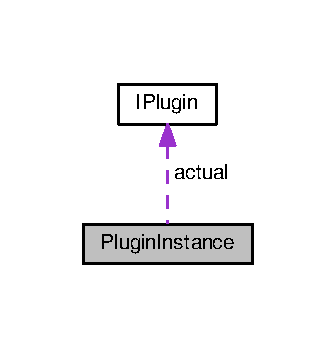
\includegraphics[width=161pt]{class_plugin_instance__coll__graph}
\end{center}
\end{figure}
\subsection*{Classes}
\begin{DoxyCompactItemize}
\item 
class \hyperlink{class_plugin_instance_1_1_impl}{Impl}
\end{DoxyCompactItemize}
\subsection*{Public Member Functions}
\begin{DoxyCompactItemize}
\item 
\mbox{\Hypertarget{class_plugin_instance_a07bf9ea0de251fd6435c8744cc1e90ec}\label{class_plugin_instance_a07bf9ea0de251fd6435c8744cc1e90ec}} 
{\bfseries Plugin\+Instance} (const std\+::string \&name)
\item 
\mbox{\Hypertarget{class_plugin_instance_a1323b013242884d9537f9e1f04b2b108}\label{class_plugin_instance_a1323b013242884d9537f9e1f04b2b108}} 
bool \hyperlink{class_plugin_instance_a1323b013242884d9537f9e1f04b2b108}{Load} ()
\begin{DoxyCompactList}\small\item\em Load the plugin. \end{DoxyCompactList}\item 
\mbox{\Hypertarget{class_plugin_instance_aab005c3fdaa2fc27e75fb71b5de6671c}\label{class_plugin_instance_aab005c3fdaa2fc27e75fb71b5de6671c}} 
bool \hyperlink{class_plugin_instance_aab005c3fdaa2fc27e75fb71b5de6671c}{Unload} ()
\begin{DoxyCompactList}\small\item\em Unload the plugin. \end{DoxyCompactList}\item 
\mbox{\Hypertarget{class_plugin_instance_ad1ba2711ffe606b85540ff24e4fe6f03}\label{class_plugin_instance_ad1ba2711ffe606b85540ff24e4fe6f03}} 
bool \hyperlink{class_plugin_instance_ad1ba2711ffe606b85540ff24e4fe6f03}{Is\+Loaded} ()
\begin{DoxyCompactList}\small\item\em Return true if the plugin is loaded. \end{DoxyCompactList}\item 
\mbox{\Hypertarget{class_plugin_instance_a8236f5136a747e8ff9f5e122fbb13033}\label{class_plugin_instance_a8236f5136a747e8ff9f5e122fbb13033}} 
std\+::string \hyperlink{class_plugin_instance_a8236f5136a747e8ff9f5e122fbb13033}{Get\+File\+Name} ()
\begin{DoxyCompactList}\small\item\em Return the path to the plugin file on disk. \end{DoxyCompactList}\item 
\mbox{\Hypertarget{class_plugin_instance_a7a1964ff60e001535bae1e4bdcbfe62f}\label{class_plugin_instance_a7a1964ff60e001535bae1e4bdcbfe62f}} 
std\+::string \hyperlink{class_plugin_instance_a7a1964ff60e001535bae1e4bdcbfe62f}{Get\+Display\+Name} ()
\begin{DoxyCompactList}\small\item\em Return the display name for the plugin. \end{DoxyCompactList}\end{DoxyCompactItemize}
\subsection*{Public Attributes}
\begin{DoxyCompactItemize}
\item 
\mbox{\Hypertarget{class_plugin_instance_ae9a6b5246d5daf974d12a15c7949407b}\label{class_plugin_instance_ae9a6b5246d5daf974d12a15c7949407b}} 
\hyperlink{class_i_plugin}{I\+Plugin} $\ast$ \hyperlink{class_plugin_instance_ae9a6b5246d5daf974d12a15c7949407b}{actual}
\begin{DoxyCompactList}\small\item\em Pointer to the actual plugin instance. \end{DoxyCompactList}\end{DoxyCompactItemize}


\subsection{Detailed Description}
C\+O\+R\+E\+\_\+\+A\+PI \hyperlink{class_plugin_instance}{Plugin\+Instance}. 

An object to represent a single plugin in the system

\begin{DoxyAuthor}{Author}
Patrick Heyer, \href{mailto:patrickhey@prodigy.net.mx}{\tt patrickhey@prodigy.\+net.\+mx} 
\end{DoxyAuthor}
\begin{DoxyDate}{Date}
jul 13, 2014 
\end{DoxyDate}
\begin{DoxyVersion}{Version}
1.\+0 
\end{DoxyVersion}


Definition at line 28 of file pluginmanager.\+h.



The documentation for this class was generated from the following files\+:\begin{DoxyCompactItemize}
\item 
/home/patrick/projects/\+Gesture\+\_\+\+Therapy\+\_\+\+Linux/src/\+Plugin\+\_\+\+A\+P\+I/\hyperlink{pluginmanager_8h}{pluginmanager.\+h}\item 
/home/patrick/projects/\+Gesture\+\_\+\+Therapy\+\_\+\+Linux/src/\+Plugin\+\_\+\+A\+P\+I/pluginmanager.\+cpp\end{DoxyCompactItemize}

\hypertarget{class_plugin_manager}{}\section{Plugin\+Manager Class Reference}
\label{class_plugin_manager}\index{Plugin\+Manager@{Plugin\+Manager}}


C\+O\+R\+E\+\_\+\+A\+PI \hyperlink{class_plugin_manager}{Plugin\+Manager}.  




{\ttfamily \#include $<$pluginmanager.\+h$>$}

\subsection*{Public Member Functions}
\begin{DoxyCompactItemize}
\item 
\mbox{\Hypertarget{class_plugin_manager_a9cfa0cf37c1f03371d83f56d48b26884}\label{class_plugin_manager_a9cfa0cf37c1f03371d83f56d48b26884}} 
bool \hyperlink{class_plugin_manager_a9cfa0cf37c1f03371d83f56d48b26884}{Load} (const std\+::string \&name)
\begin{DoxyCompactList}\small\item\em Load a single plugin by name. \end{DoxyCompactList}\item 
\mbox{\Hypertarget{class_plugin_manager_acf215381606a14747a8a0766bef9e1f1}\label{class_plugin_manager_acf215381606a14747a8a0766bef9e1f1}} 
bool \hyperlink{class_plugin_manager_acf215381606a14747a8a0766bef9e1f1}{Load\+From\+File} (const std\+::string \&filename)
\begin{DoxyCompactList}\small\item\em load a list of plugins by name from file \end{DoxyCompactList}\item 
\mbox{\Hypertarget{class_plugin_manager_a956e653b7db36da9d034b4a93c8308d5}\label{class_plugin_manager_a956e653b7db36da9d034b4a93c8308d5}} 
bool \hyperlink{class_plugin_manager_a956e653b7db36da9d034b4a93c8308d5}{Initialize} (const std\+::string \&name)
\begin{DoxyCompactList}\small\item\em Initialize a single plugin by name. \end{DoxyCompactList}\item 
\mbox{\Hypertarget{class_plugin_manager_a66bbd81ad0771e495af91718c0c58859}\label{class_plugin_manager_a66bbd81ad0771e495af91718c0c58859}} 
bool \hyperlink{class_plugin_manager_a66bbd81ad0771e495af91718c0c58859}{Initialize\+All} ()
\begin{DoxyCompactList}\small\item\em Initialize all plugins in m\+Plugins. \end{DoxyCompactList}\item 
\mbox{\Hypertarget{class_plugin_manager_ab7ac61ad5e567af6ed38574cb89e80e6}\label{class_plugin_manager_ab7ac61ad5e567af6ed38574cb89e80e6}} 
bool \hyperlink{class_plugin_manager_ab7ac61ad5e567af6ed38574cb89e80e6}{Execute} (const std\+::string \&name)
\begin{DoxyCompactList}\small\item\em Execute a single plugin by name. \end{DoxyCompactList}\item 
\mbox{\Hypertarget{class_plugin_manager_ad2c750b62404561213e397066b852abb}\label{class_plugin_manager_ad2c750b62404561213e397066b852abb}} 
bool \hyperlink{class_plugin_manager_ad2c750b62404561213e397066b852abb}{Execute\+All} ()
\begin{DoxyCompactList}\small\item\em Execute all plugins in m\+Plugins. \end{DoxyCompactList}\item 
\mbox{\Hypertarget{class_plugin_manager_ab651a05d6fcb92562807e9f5ecc30855}\label{class_plugin_manager_ab651a05d6fcb92562807e9f5ecc30855}} 
bool \hyperlink{class_plugin_manager_ab651a05d6fcb92562807e9f5ecc30855}{Unload} (const std\+::string \&name)
\begin{DoxyCompactList}\small\item\em Unload a single plugin by name. \end{DoxyCompactList}\item 
\mbox{\Hypertarget{class_plugin_manager_ac771065cfdf4032cfb254d2ae2cb0c0f}\label{class_plugin_manager_ac771065cfdf4032cfb254d2ae2cb0c0f}} 
bool \hyperlink{class_plugin_manager_ac771065cfdf4032cfb254d2ae2cb0c0f}{Unload\+All} ()
\begin{DoxyCompactList}\small\item\em Unload all plugins. \end{DoxyCompactList}\end{DoxyCompactItemize}
\subsection*{Static Public Member Functions}
\begin{DoxyCompactItemize}
\item 
\mbox{\Hypertarget{class_plugin_manager_acc7641f5801a2df305dc71e1e87fc25b}\label{class_plugin_manager_acc7641f5801a2df305dc71e1e87fc25b}} 
static \hyperlink{class_plugin_manager}{Plugin\+Manager} \& \hyperlink{class_plugin_manager_acc7641f5801a2df305dc71e1e87fc25b}{get\+Instance} ()
\begin{DoxyCompactList}\small\item\em Return the single instance of the plugin manager. \end{DoxyCompactList}\end{DoxyCompactItemize}


\subsection{Detailed Description}
C\+O\+R\+E\+\_\+\+A\+PI \hyperlink{class_plugin_manager}{Plugin\+Manager}. 

A manger for all plugins in the Core A\+PI using singleton pattern to avoid multiple instances

\begin{DoxyAuthor}{Author}
Patrick Heyer, \href{mailto:patrickhey@prodigy.net.mx}{\tt patrickhey@prodigy.\+net.\+mx} 
\end{DoxyAuthor}
\begin{DoxyDate}{Date}
jul 13, 2014 
\end{DoxyDate}
\begin{DoxyVersion}{Version}
1.\+0 
\end{DoxyVersion}


Definition at line 67 of file pluginmanager.\+h.



The documentation for this class was generated from the following files\+:\begin{DoxyCompactItemize}
\item 
/home/patrick/projects/\+Gesture\+\_\+\+Therapy\+\_\+\+Linux/src/\+Plugin\+\_\+\+A\+P\+I/\hyperlink{pluginmanager_8h}{pluginmanager.\+h}\item 
/home/patrick/projects/\+Gesture\+\_\+\+Therapy\+\_\+\+Linux/src/\+Plugin\+\_\+\+A\+P\+I/pluginmanager.\+cpp\end{DoxyCompactItemize}

\hypertarget{class_screen___reader}{}\section{Screen\+\_\+\+Reader Class Reference}
\label{class_screen___reader}\index{Screen\+\_\+\+Reader@{Screen\+\_\+\+Reader}}


\hyperlink{class_screen___reader}{Screen\+\_\+\+Reader} plugin.  




Inheritance diagram for Screen\+\_\+\+Reader\+:\nopagebreak
\begin{figure}[H]
\begin{center}
\leavevmode
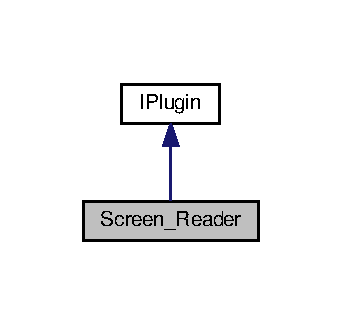
\includegraphics[width=164pt]{class_screen___reader__inherit__graph}
\end{center}
\end{figure}


Collaboration diagram for Screen\+\_\+\+Reader\+:\nopagebreak
\begin{figure}[H]
\begin{center}
\leavevmode
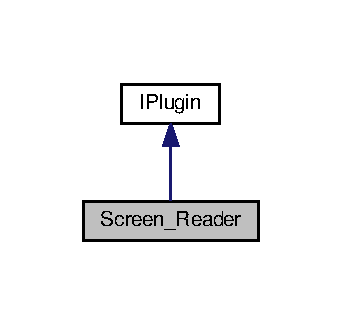
\includegraphics[width=164pt]{class_screen___reader__coll__graph}
\end{center}
\end{figure}
\subsection*{Public Member Functions}
\begin{DoxyCompactItemize}
\item 
void \hyperlink{class_screen___reader_add5cdfdc432ed5e8baa6683213c6daba}{Main} ()
\begin{DoxyCompactList}\small\item\em Main funcction of the plugin. \end{DoxyCompactList}\item 
bool \hyperlink{class_screen___reader_aaae80932d8f6af903ca93846eb4de234}{load\+Configuration} ()
\begin{DoxyCompactList}\small\item\em Load configuration. \end{DoxyCompactList}\item 
bool \hyperlink{class_screen___reader_a6d211f9c63493fbc1b18fd780f61dcdc}{save\+Configuration} ()
\begin{DoxyCompactList}\small\item\em Save configuration. \end{DoxyCompactList}\item 
bool \hyperlink{class_screen___reader_ab6219f6991a1574fb20b5f96953da62e}{Initialize\+\_\+\+Output} ()
\begin{DoxyCompactList}\small\item\em Initialize Output variables for the plugin to publish. \end{DoxyCompactList}\item 
bool \hyperlink{class_screen___reader_a40c7e767ec368074d63ba4d4e5e3e0bc}{Initialize\+\_\+\+Input} ()
\begin{DoxyCompactList}\small\item\em Initialize Input variables for the plugin to publish. \end{DoxyCompactList}\item 
void \hyperlink{class_screen___reader_a40e260696012cdb8ab05d65511b7de6e}{stop} ()
\begin{DoxyCompactList}\small\item\em Stop plugin. \end{DoxyCompactList}\item 
void \hyperlink{class_screen___reader_a9c716b5a3b6f94e1cf89eee7823ecd60}{run} ()
\begin{DoxyCompactList}\small\item\em Execute plugin. \end{DoxyCompactList}\end{DoxyCompactItemize}
\subsection*{Additional Inherited Members}


\subsection{Detailed Description}
\hyperlink{class_screen___reader}{Screen\+\_\+\+Reader} plugin. 

This plugin is a legacy wrapper that alows us to use Hocoma\textquotesingle{}s games with this architecture it writes output to a shared memory segment defined by hocoma that can not be changed \begin{DoxyAuthor}{Author}
Patrick Heyer, \href{mailto:patrickhey@prodigy.net.mx}{\tt patrickhey@prodigy.\+net.\+mx} 
\end{DoxyAuthor}
\begin{DoxyDate}{Date}
jul 13, 2014 
\end{DoxyDate}
\begin{DoxyVersion}{Version}
1.\+0 
\end{DoxyVersion}


Definition at line 38 of file Main.\+cpp.



\subsection{Member Function Documentation}
\mbox{\Hypertarget{class_screen___reader_a40c7e767ec368074d63ba4d4e5e3e0bc}\label{class_screen___reader_a40c7e767ec368074d63ba4d4e5e3e0bc}} 
\index{Screen\+\_\+\+Reader@{Screen\+\_\+\+Reader}!Initialize\+\_\+\+Input@{Initialize\+\_\+\+Input}}
\index{Initialize\+\_\+\+Input@{Initialize\+\_\+\+Input}!Screen\+\_\+\+Reader@{Screen\+\_\+\+Reader}}
\subsubsection{\texorpdfstring{Initialize\+\_\+\+Input()}{Initialize\_Input()}}
{\footnotesize\ttfamily bool Screen\+\_\+\+Reader\+::\+Initialize\+\_\+\+Input (\begin{DoxyParamCaption}{ }\end{DoxyParamCaption})\hspace{0.3cm}{\ttfamily [virtual]}}



Initialize Input variables for the plugin to publish. 

\begin{DoxyReturn}{Returns}
bool 
\end{DoxyReturn}


Implements \hyperlink{class_i_plugin_aa7c66743ad956d8ada57becee559af4d}{I\+Plugin}.



Definition at line 149 of file Main.\+cpp.


\begin{DoxyCode}
150 \{
151     Plugin\_ERROR = Shared\_Memory::getInstance().Register\_String\_Input(\textcolor{stringliteral}{"Plugin\_ERROR"});
152     \textcolor{keywordflow}{return} \textcolor{keyword}{true};
153 \}
\end{DoxyCode}
\mbox{\Hypertarget{class_screen___reader_ab6219f6991a1574fb20b5f96953da62e}\label{class_screen___reader_ab6219f6991a1574fb20b5f96953da62e}} 
\index{Screen\+\_\+\+Reader@{Screen\+\_\+\+Reader}!Initialize\+\_\+\+Output@{Initialize\+\_\+\+Output}}
\index{Initialize\+\_\+\+Output@{Initialize\+\_\+\+Output}!Screen\+\_\+\+Reader@{Screen\+\_\+\+Reader}}
\subsubsection{\texorpdfstring{Initialize\+\_\+\+Output()}{Initialize\_Output()}}
{\footnotesize\ttfamily bool Screen\+\_\+\+Reader\+::\+Initialize\+\_\+\+Output (\begin{DoxyParamCaption}{ }\end{DoxyParamCaption})\hspace{0.3cm}{\ttfamily [virtual]}}



Initialize Output variables for the plugin to publish. 

\begin{DoxyReturn}{Returns}
bool 
\end{DoxyReturn}


Implements \hyperlink{class_i_plugin_a0b772513fc8c4ed01240e19c4bb84068}{I\+Plugin}.



Definition at line 142 of file Main.\+cpp.


\begin{DoxyCode}
143 \{   
144     
145     Shared\_Memory::getInstance().Register\_Output(\textcolor{stringliteral}{"Video\_From\_Screen"}, &frame);
146     \textcolor{keywordflow}{return} \textcolor{keyword}{true};
147 \}
\end{DoxyCode}
\mbox{\Hypertarget{class_screen___reader_aaae80932d8f6af903ca93846eb4de234}\label{class_screen___reader_aaae80932d8f6af903ca93846eb4de234}} 
\index{Screen\+\_\+\+Reader@{Screen\+\_\+\+Reader}!load\+Configuration@{load\+Configuration}}
\index{load\+Configuration@{load\+Configuration}!Screen\+\_\+\+Reader@{Screen\+\_\+\+Reader}}
\subsubsection{\texorpdfstring{load\+Configuration()}{loadConfiguration()}}
{\footnotesize\ttfamily bool Screen\+\_\+\+Reader\+::load\+Configuration (\begin{DoxyParamCaption}{ }\end{DoxyParamCaption})\hspace{0.3cm}{\ttfamily [virtual]}}



Load configuration. 

The configuration can be loaded from file, or be hard coded into the plugin (not recomended), initialization of public and private variables should occur here

By default load\+Configuration is called during \hyperlink{class_plugin_manager_a956e653b7db36da9d034b4a93c8308d5}{Plugin\+Manager\+::\+Initialize()} by the plugin manager.

\begin{DoxyReturn}{Returns}
bool 
\end{DoxyReturn}


Implements \hyperlink{class_i_plugin_a418cff309436d3a15d9a4ce7369db6dd}{I\+Plugin}.



Definition at line 132 of file Main.\+cpp.


\begin{DoxyCode}
133 \{
134     \textcolor{keywordflow}{return} \textcolor{keyword}{true};
135 \}
\end{DoxyCode}
\mbox{\Hypertarget{class_screen___reader_add5cdfdc432ed5e8baa6683213c6daba}\label{class_screen___reader_add5cdfdc432ed5e8baa6683213c6daba}} 
\index{Screen\+\_\+\+Reader@{Screen\+\_\+\+Reader}!Main@{Main}}
\index{Main@{Main}!Screen\+\_\+\+Reader@{Screen\+\_\+\+Reader}}
\subsubsection{\texorpdfstring{Main()}{Main()}}
{\footnotesize\ttfamily void Screen\+\_\+\+Reader\+::\+Main (\begin{DoxyParamCaption}{ }\end{DoxyParamCaption})\hspace{0.3cm}{\ttfamily [virtual]}}



Main funcction of the plugin. 

Started in a new thread by the Run() funcction is the most importatn funcction of the plugin. Infinite loop (generaly a while(running) function that runs undefenitly in a read/process/write cicle). \begin{DoxyReturn}{Returns}
void 
\end{DoxyReturn}


Implements \hyperlink{class_i_plugin_ab5fdb3b0f7afdcee04324dca01766749}{I\+Plugin}.



Definition at line 116 of file Main.\+cpp.


\begin{DoxyCode}
117 \{
118     Mat img;
119     \textcolor{keywordflow}{while} (running)
120     \{
121         \hyperlink{struct_screen_shot}{ScreenShot} screen(0,0,1366,768);               
122         screen(img);        
123        \textcolor{comment}{// imshow("Screen", img);}
124         usleep(1000);
125         
126     \}
127     
128     stoped = \textcolor{keyword}{true};
129     \textcolor{keywordflow}{return};
130 \}
\end{DoxyCode}
\mbox{\Hypertarget{class_screen___reader_a9c716b5a3b6f94e1cf89eee7823ecd60}\label{class_screen___reader_a9c716b5a3b6f94e1cf89eee7823ecd60}} 
\index{Screen\+\_\+\+Reader@{Screen\+\_\+\+Reader}!run@{run}}
\index{run@{run}!Screen\+\_\+\+Reader@{Screen\+\_\+\+Reader}}
\subsubsection{\texorpdfstring{run()}{run()}}
{\footnotesize\ttfamily void Screen\+\_\+\+Reader\+::run (\begin{DoxyParamCaption}{ }\end{DoxyParamCaption})\hspace{0.3cm}{\ttfamily [virtual]}}



Execute plugin. 

Starts a new thread and executes the plugins main() funcction. \begin{DoxyReturn}{Returns}
void 
\end{DoxyReturn}


Implements \hyperlink{class_i_plugin_a46b4ace767e77f9db9c9585e99c09039}{I\+Plugin}.



Definition at line 155 of file Main.\+cpp.



References I\+Plugin\+::\+Inc\+Wrapper().


\begin{DoxyCode}
156 \{
157     pthread\_create(&thread\_id, NULL, &\hyperlink{class_i_plugin_a62d22be2fdf66eb7f5c2f797f5f3d7f3}{IPlugin::IncWrapper}, \textcolor{keyword}{this});
158     running = \textcolor{keyword}{true};
159     stoped = \textcolor{keyword}{false};
160 \}
\end{DoxyCode}
\mbox{\Hypertarget{class_screen___reader_a6d211f9c63493fbc1b18fd780f61dcdc}\label{class_screen___reader_a6d211f9c63493fbc1b18fd780f61dcdc}} 
\index{Screen\+\_\+\+Reader@{Screen\+\_\+\+Reader}!save\+Configuration@{save\+Configuration}}
\index{save\+Configuration@{save\+Configuration}!Screen\+\_\+\+Reader@{Screen\+\_\+\+Reader}}
\subsubsection{\texorpdfstring{save\+Configuration()}{saveConfiguration()}}
{\footnotesize\ttfamily bool Screen\+\_\+\+Reader\+::save\+Configuration (\begin{DoxyParamCaption}{ }\end{DoxyParamCaption})\hspace{0.3cm}{\ttfamily [virtual]}}



Save configuration. 

The configuration should be saved to file, public and private variables that should be configured at startup should be saved.

By default save\+Configuration is called during \hyperlink{class_plugin_manager_ab651a05d6fcb92562807e9f5ecc30855}{Plugin\+Manager\+::\+Unload()} by the plugin manager.

\begin{DoxyReturn}{Returns}
bool 
\end{DoxyReturn}


Implements \hyperlink{class_i_plugin_a79b5c42b1c7b08257a6110b2091039bc}{I\+Plugin}.



Definition at line 137 of file Main.\+cpp.


\begin{DoxyCode}
138 \{
139     \textcolor{keywordflow}{return} \textcolor{keyword}{true};
140 \}
\end{DoxyCode}
\mbox{\Hypertarget{class_screen___reader_a40e260696012cdb8ab05d65511b7de6e}\label{class_screen___reader_a40e260696012cdb8ab05d65511b7de6e}} 
\index{Screen\+\_\+\+Reader@{Screen\+\_\+\+Reader}!stop@{stop}}
\index{stop@{stop}!Screen\+\_\+\+Reader@{Screen\+\_\+\+Reader}}
\subsubsection{\texorpdfstring{stop()}{stop()}}
{\footnotesize\ttfamily void Screen\+\_\+\+Reader\+::stop (\begin{DoxyParamCaption}{ }\end{DoxyParamCaption})\hspace{0.3cm}{\ttfamily [virtual]}}



Stop plugin. 

Stops the plugin \begin{DoxyReturn}{Returns}
void 
\end{DoxyReturn}


Implements \hyperlink{class_i_plugin_a86e523c283aec5c9fb21249a76e916ac}{I\+Plugin}.



Definition at line 162 of file Main.\+cpp.


\begin{DoxyCode}
163 \{
164     running = \textcolor{keyword}{false};
165 \}
\end{DoxyCode}


The documentation for this class was generated from the following file\+:\begin{DoxyCompactItemize}
\item 
/home/patrick/projects/\+Gesture\+\_\+\+Therapy\+\_\+\+Linux/src/\+Screen\+\_\+\+Reader/Main.\+cpp\end{DoxyCompactItemize}

\hypertarget{struct_screen_shot}{}\section{Screen\+Shot Struct Reference}
\label{struct_screen_shot}\index{Screen\+Shot@{Screen\+Shot}}
\subsection*{Public Member Functions}
\begin{DoxyCompactItemize}
\item 
\mbox{\Hypertarget{struct_screen_shot_a420ab4091f09cc75b24e4acea4fade77}\label{struct_screen_shot_a420ab4091f09cc75b24e4acea4fade77}} 
{\bfseries Screen\+Shot} (int x, int y, int width, int height)
\item 
\mbox{\Hypertarget{struct_screen_shot_af97cd69859cfcd495789c5bfa5dc87a4}\label{struct_screen_shot_af97cd69859cfcd495789c5bfa5dc87a4}} 
void {\bfseries operator()} (Mat \&cv\+Img)
\end{DoxyCompactItemize}
\subsection*{Public Attributes}
\begin{DoxyCompactItemize}
\item 
\mbox{\Hypertarget{struct_screen_shot_a5c431da3dc18806f4925353ca43c9089}\label{struct_screen_shot_a5c431da3dc18806f4925353ca43c9089}} 
Display $\ast$ {\bfseries display}
\item 
\mbox{\Hypertarget{struct_screen_shot_a3c66eb4571cd1e5113b656fb3ac8820b}\label{struct_screen_shot_a3c66eb4571cd1e5113b656fb3ac8820b}} 
Window {\bfseries root}
\item 
\mbox{\Hypertarget{struct_screen_shot_af2da7df6098097be3a51499fab3cdacf}\label{struct_screen_shot_af2da7df6098097be3a51499fab3cdacf}} 
int {\bfseries x}
\item 
\mbox{\Hypertarget{struct_screen_shot_a06e8ca521c0ba57825197e9c5aba1d9b}\label{struct_screen_shot_a06e8ca521c0ba57825197e9c5aba1d9b}} 
int {\bfseries y}
\item 
\mbox{\Hypertarget{struct_screen_shot_a0f783746a74ae0d6c848495261094925}\label{struct_screen_shot_a0f783746a74ae0d6c848495261094925}} 
int {\bfseries width}
\item 
\mbox{\Hypertarget{struct_screen_shot_ae38af2dd0b09e3be27f465941edf8418}\label{struct_screen_shot_ae38af2dd0b09e3be27f465941edf8418}} 
int {\bfseries height}
\item 
\mbox{\Hypertarget{struct_screen_shot_aaf21aa932effe1876b5c4a2c52d5b77b}\label{struct_screen_shot_aaf21aa932effe1876b5c4a2c52d5b77b}} 
X\+Image $\ast$ {\bfseries img}
\item 
\mbox{\Hypertarget{struct_screen_shot_a05cbf0b41abb03d8c038ad3ccbb8fc64}\label{struct_screen_shot_a05cbf0b41abb03d8c038ad3ccbb8fc64}} 
bool {\bfseries init}
\end{DoxyCompactItemize}


\subsection{Detailed Description}


Definition at line 76 of file Main.\+cpp.



The documentation for this struct was generated from the following file\+:\begin{DoxyCompactItemize}
\item 
/home/patrick/projects/\+Gesture\+\_\+\+Therapy\+\_\+\+Linux/src/\+Screen\+\_\+\+Reader/Main.\+cpp\end{DoxyCompactItemize}

\hypertarget{class_shared___memory}{}\section{Shared\+\_\+\+Memory Class Reference}
\label{class_shared___memory}\index{Shared\+\_\+\+Memory@{Shared\+\_\+\+Memory}}
\subsection*{Public Member Functions}
\begin{DoxyCompactItemize}
\item 
\mbox{\Hypertarget{class_shared___memory_aa056d584c6ff778d0e3e6a49bae982e1}\label{class_shared___memory_aa056d584c6ff778d0e3e6a49bae982e1}} 
void {\bfseries Initialize} (void)
\item 
\mbox{\Hypertarget{class_shared___memory_ac1a0a9ba0b7ea383dc937f5e01ce301c}\label{class_shared___memory_ac1a0a9ba0b7ea383dc937f5e01ce301c}} 
void {\bfseries Register\+\_\+\+Output} (std\+::string name, bool $\ast$value)
\item 
\mbox{\Hypertarget{class_shared___memory_a1e89435b0ae24bf9ea8dbececf7bf01a}\label{class_shared___memory_a1e89435b0ae24bf9ea8dbececf7bf01a}} 
bool $\ast$ {\bfseries Register\+\_\+\+Bool\+\_\+\+Input} (std\+::string name)
\item 
\mbox{\Hypertarget{class_shared___memory_af1354075089c0e0feeb817a528ea954c}\label{class_shared___memory_af1354075089c0e0feeb817a528ea954c}} 
void {\bfseries Register\+\_\+\+Output} (std\+::string name, char $\ast$value)
\item 
\mbox{\Hypertarget{class_shared___memory_a9025a9c7b5340e2018c2b0787600567c}\label{class_shared___memory_a9025a9c7b5340e2018c2b0787600567c}} 
char $\ast$ {\bfseries Register\+\_\+\+Char\+\_\+\+Input} (std\+::string name)
\item 
\mbox{\Hypertarget{class_shared___memory_ad93f804cfa69d53394f65590d318f8f4}\label{class_shared___memory_ad93f804cfa69d53394f65590d318f8f4}} 
void {\bfseries Register\+\_\+\+Output} (std\+::string name, double $\ast$value)
\item 
\mbox{\Hypertarget{class_shared___memory_afd0446ab3118d9f1582da04296809a7d}\label{class_shared___memory_afd0446ab3118d9f1582da04296809a7d}} 
double $\ast$ {\bfseries Register\+\_\+\+Double\+\_\+\+Input} (std\+::string name)
\item 
\mbox{\Hypertarget{class_shared___memory_ae91ffb0fa801d256e45f64e48ba173f2}\label{class_shared___memory_ae91ffb0fa801d256e45f64e48ba173f2}} 
void {\bfseries Register\+\_\+\+Output} (std\+::string name, float $\ast$value)
\item 
\mbox{\Hypertarget{class_shared___memory_ac1eba064511b1dc5ae2927c0bd683762}\label{class_shared___memory_ac1eba064511b1dc5ae2927c0bd683762}} 
float $\ast$ {\bfseries Register\+\_\+\+Float\+\_\+\+Input} (std\+::string name)
\item 
\mbox{\Hypertarget{class_shared___memory_aa6e367a3e1076e8e392e1a4291de3062}\label{class_shared___memory_aa6e367a3e1076e8e392e1a4291de3062}} 
void {\bfseries Register\+\_\+\+Output} (std\+::string name, int $\ast$value)
\item 
\mbox{\Hypertarget{class_shared___memory_a7000ec66a0d8679b91d78535e65974f5}\label{class_shared___memory_a7000ec66a0d8679b91d78535e65974f5}} 
int $\ast$ {\bfseries Register\+\_\+\+Int\+\_\+\+Input} (std\+::string name)
\item 
\mbox{\Hypertarget{class_shared___memory_a894da19d9977b3e7618ad22e68964666}\label{class_shared___memory_a894da19d9977b3e7618ad22e68964666}} 
void {\bfseries Register\+\_\+\+Output} (std\+::string name, long $\ast$value)
\item 
\mbox{\Hypertarget{class_shared___memory_a51d5425a6a2557bca0463cb8d28a7a54}\label{class_shared___memory_a51d5425a6a2557bca0463cb8d28a7a54}} 
long $\ast$ {\bfseries Register\+\_\+\+Long\+\_\+\+Input} (std\+::string name)
\item 
\mbox{\Hypertarget{class_shared___memory_a0a7cc51cffb7dde7fdcbab18b32defec}\label{class_shared___memory_a0a7cc51cffb7dde7fdcbab18b32defec}} 
void {\bfseries Register\+\_\+\+Output} (std\+::string name, std\+::string $\ast$value)
\item 
\mbox{\Hypertarget{class_shared___memory_a45ffc5e30b6d680faf99a02fadbfe09a}\label{class_shared___memory_a45ffc5e30b6d680faf99a02fadbfe09a}} 
std\+::string $\ast$ {\bfseries Register\+\_\+\+String\+\_\+\+Input} (std\+::string name)
\item 
\mbox{\Hypertarget{class_shared___memory_a9a1859f2488f225234e86d3da2654c65}\label{class_shared___memory_a9a1859f2488f225234e86d3da2654c65}} 
void {\bfseries Register\+\_\+\+Output} (std\+::string name, void $\ast$value)
\item 
\mbox{\Hypertarget{class_shared___memory_a6a75d34f8611b57e8c5ee0708cc8c4e6}\label{class_shared___memory_a6a75d34f8611b57e8c5ee0708cc8c4e6}} 
void $\ast$ {\bfseries Register\+\_\+\+Void\+\_\+\+Input} (std\+::string name)
\item 
\mbox{\Hypertarget{class_shared___memory_a5d0f14cd98f9cd12040d859560cb4d1a}\label{class_shared___memory_a5d0f14cd98f9cd12040d859560cb4d1a}} 
void {\bfseries Register\+\_\+\+Output} (std\+::string name, std\+::function$<$ void(std\+::vector$<$ std\+::string $>$ i\+\_\+params, std\+::vector$<$ std\+::string $>$ o\+\_\+params)$>$ value)
\item 
\mbox{\Hypertarget{class_shared___memory_a14c12d9dda3a4693c7589baeec1f4ca9}\label{class_shared___memory_a14c12d9dda3a4693c7589baeec1f4ca9}} 
std\+::function$<$ void(std\+::vector$<$ std\+::string $>$ i\+\_\+params, std\+::vector$<$ std\+::string $>$ o\+\_\+params)$>$ {\bfseries Register\+\_\+\+Func\+\_\+\+Input} (std\+::string name)
\end{DoxyCompactItemize}
\subsection*{Static Public Member Functions}
\begin{DoxyCompactItemize}
\item 
\mbox{\Hypertarget{class_shared___memory_a74b498d41295b1dd006ac6f1f0b6065d}\label{class_shared___memory_a74b498d41295b1dd006ac6f1f0b6065d}} 
static \hyperlink{class_shared___memory}{Shared\+\_\+\+Memory} \& {\bfseries get\+Instance} ()
\item 
\mbox{\Hypertarget{class_shared___memory_af232a41a63eac5a08f762400e8086052}\label{class_shared___memory_af232a41a63eac5a08f762400e8086052}} 
static void {\bfseries free\+Instance} (void)
\end{DoxyCompactItemize}
\subsection*{Public Attributes}
\begin{DoxyCompactItemize}
\item 
\mbox{\Hypertarget{class_shared___memory_a319123cd69aac705bcc43b071f9dc21c}\label{class_shared___memory_a319123cd69aac705bcc43b071f9dc21c}} 
std\+::map$<$ std\+::string, double $\ast$ $>$ {\bfseries List\+\_\+\+Doubles}
\item 
\mbox{\Hypertarget{class_shared___memory_a153131243072a8bd88a9361e16f84473}\label{class_shared___memory_a153131243072a8bd88a9361e16f84473}} 
std\+::map$<$ std\+::string, float $\ast$ $>$ {\bfseries List\+\_\+\+Floats}
\item 
\mbox{\Hypertarget{class_shared___memory_ac9a6608511056e00f726d2b7ffe7696e}\label{class_shared___memory_ac9a6608511056e00f726d2b7ffe7696e}} 
std\+::map$<$ std\+::string, int $\ast$ $>$ {\bfseries List\+\_\+\+Ints}
\item 
\mbox{\Hypertarget{class_shared___memory_a3f22062cdd9ce8e6259aa3929f3bffb4}\label{class_shared___memory_a3f22062cdd9ce8e6259aa3929f3bffb4}} 
std\+::map$<$ std\+::string, long $\ast$ $>$ {\bfseries List\+\_\+\+Longs}
\item 
\mbox{\Hypertarget{class_shared___memory_ae452e5b93bc5c8068ea06a9375bd7ba7}\label{class_shared___memory_ae452e5b93bc5c8068ea06a9375bd7ba7}} 
std\+::map$<$ std\+::string, bool $\ast$ $>$ {\bfseries List\+\_\+\+Bools}
\item 
\mbox{\Hypertarget{class_shared___memory_a554c2ceb1bfdd15aff4ef99c9ef9e52d}\label{class_shared___memory_a554c2ceb1bfdd15aff4ef99c9ef9e52d}} 
std\+::map$<$ std\+::string, char $\ast$ $>$ {\bfseries List\+\_\+\+Chars}
\item 
\mbox{\Hypertarget{class_shared___memory_aab4d6f0ea3556d678d2ddca9783475d2}\label{class_shared___memory_aab4d6f0ea3556d678d2ddca9783475d2}} 
std\+::map$<$ std\+::string, std\+::string $\ast$ $>$ {\bfseries List\+\_\+\+Strings}
\item 
\mbox{\Hypertarget{class_shared___memory_a2985f2c3d83e9035e50ca2eae5eed0b8}\label{class_shared___memory_a2985f2c3d83e9035e50ca2eae5eed0b8}} 
std\+::map$<$ std\+::string, void $\ast$ $>$ {\bfseries List\+\_\+\+Voids}
\item 
\mbox{\Hypertarget{class_shared___memory_aae8d26d1cc1344574471397191a17c23}\label{class_shared___memory_aae8d26d1cc1344574471397191a17c23}} 
std\+::map$<$ std\+::string, std\+::function$<$ void(std\+::vector$<$ std\+::string $>$ i\+\_\+params, std\+::vector$<$ std\+::string $>$ o\+\_\+params)$>$ $>$ {\bfseries List\+\_\+\+Funcs}
\end{DoxyCompactItemize}
\subsection*{Protected Member Functions}
\begin{DoxyCompactItemize}
\item 
\mbox{\Hypertarget{class_shared___memory_ad9f7e3225b081f872874c2f0d29e2232}\label{class_shared___memory_ad9f7e3225b081f872874c2f0d29e2232}} 
{\bfseries Shared\+\_\+\+Memory} (const \hyperlink{class_shared___memory}{Shared\+\_\+\+Memory} \&other)
\item 
\mbox{\Hypertarget{class_shared___memory_a1f435a59e197184d1f368ed461c68796}\label{class_shared___memory_a1f435a59e197184d1f368ed461c68796}} 
virtual \hyperlink{class_shared___memory}{Shared\+\_\+\+Memory} \& {\bfseries operator=} (const \hyperlink{class_shared___memory}{Shared\+\_\+\+Memory} \&other)
\end{DoxyCompactItemize}


\subsection{Detailed Description}


Definition at line 22 of file Shared\+\_\+\+Memory.\+h.



The documentation for this class was generated from the following files\+:\begin{DoxyCompactItemize}
\item 
/home/patrick/projects/\+Gesture\+\_\+\+Therapy\+\_\+\+Linux/src/\+Shared\+\_\+\+Memory/Shared\+\_\+\+Memory.\+h\item 
/home/patrick/projects/\+Gesture\+\_\+\+Therapy\+\_\+\+Linux/src/\+Shared\+\_\+\+Memory/Shared\+\_\+\+Memory.\+cpp\end{DoxyCompactItemize}

\hypertarget{class_thread}{}\section{Thread Class Reference}
\label{class_thread}\index{Thread@{Thread}}
\subsection*{Public Member Functions}
\begin{DoxyCompactItemize}
\item 
\mbox{\Hypertarget{class_thread_aa2132343300568b671cddcb5816dafc8}\label{class_thread_aa2132343300568b671cddcb5816dafc8}} 
void $\ast$ {\bfseries member\+Function} (void)
\item 
\mbox{\Hypertarget{class_thread_ad4ec138a1bb5b3bbe328267185720198}\label{class_thread_ad4ec138a1bb5b3bbe328267185720198}} 
void {\bfseries start\+Thread} (void)
\end{DoxyCompactItemize}
\subsection*{Static Public Member Functions}
\begin{DoxyCompactItemize}
\item 
\mbox{\Hypertarget{class_thread_a89d99192bd58b8199b84a530842174fb}\label{class_thread_a89d99192bd58b8199b84a530842174fb}} 
static void $\ast$ {\bfseries call\+Member\+Function} (void $\ast$arg)
\end{DoxyCompactItemize}


\subsection{Detailed Description}


Definition at line 2 of file thread.\+h.



The documentation for this class was generated from the following files\+:\begin{DoxyCompactItemize}
\item 
/home/patrick/projects/\+Gesture\+\_\+\+Therapy\+\_\+\+Linux/src/\+Plugin\+\_\+\+A\+P\+I/thread.\+h\item 
/home/patrick/projects/\+Gesture\+\_\+\+Therapy\+\_\+\+Linux/src/\+Plugin\+\_\+\+A\+P\+I/thread.\+cpp\end{DoxyCompactItemize}

\hypertarget{struct_triplet}{}\section{Triplet Struct Reference}
\label{struct_triplet}\index{Triplet@{Triplet}}
\subsection*{Public Member Functions}
\begin{DoxyCompactItemize}
\item 
\mbox{\Hypertarget{struct_triplet_a70457ef6a05b29f73ebcd8f9270797e3}\label{struct_triplet_a70457ef6a05b29f73ebcd8f9270797e3}} 
{\bfseries Triplet} (int u, int v, int w)
\item 
\mbox{\Hypertarget{struct_triplet_aa6d4bab5cc79da13ed8ac1797b116838}\label{struct_triplet_aa6d4bab5cc79da13ed8ac1797b116838}} 
{\bfseries Triplet} (const \hyperlink{struct_triplet}{Triplet} \&orig)
\item 
\mbox{\Hypertarget{struct_triplet_a39e9b4fa3119643737509863defa67ce}\label{struct_triplet_a39e9b4fa3119643737509863defa67ce}} 
\hyperlink{struct_triplet}{Triplet} \& {\bfseries operator=} (const \hyperlink{struct_triplet}{Triplet} \&orig)
\end{DoxyCompactItemize}
\subsection*{Public Attributes}
\begin{DoxyCompactItemize}
\item 
\mbox{\Hypertarget{struct_triplet_a8f29696c8699a74d729762bd4ac021e0}\label{struct_triplet_a8f29696c8699a74d729762bd4ac021e0}} 
int {\bfseries a}
\item 
\mbox{\Hypertarget{struct_triplet_ab04c763889df0502639bc2020f445057}\label{struct_triplet_ab04c763889df0502639bc2020f445057}} 
int {\bfseries b}
\item 
\mbox{\Hypertarget{struct_triplet_a55aeb5803c35b59e170160588c090dbb}\label{struct_triplet_a55aeb5803c35b59e170160588c090dbb}} 
int {\bfseries c}
\end{DoxyCompactItemize}


\subsection{Detailed Description}


Definition at line 8 of file Triplet.\+h.



The documentation for this struct was generated from the following file\+:\begin{DoxyCompactItemize}
\item 
/home/patrick/projects/\+Gesture\+\_\+\+Therapy\+\_\+\+Linux/src/include/Triplet.\+h\end{DoxyCompactItemize}

\hypertarget{class_tuio___client}{}\section{Tuio\+\_\+\+Client Class Reference}
\label{class_tuio___client}\index{Tuio\+\_\+\+Client@{Tuio\+\_\+\+Client}}


\hyperlink{class_tuio___client}{Tuio\+\_\+\+Client} plugin.  




Inheritance diagram for Tuio\+\_\+\+Client\+:\nopagebreak
\begin{figure}[H]
\begin{center}
\leavevmode
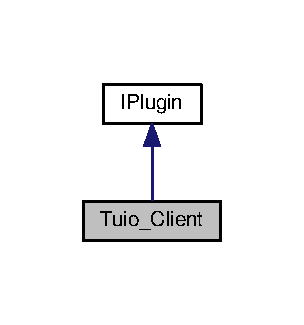
\includegraphics[width=146pt]{class_tuio___client__inherit__graph}
\end{center}
\end{figure}


Collaboration diagram for Tuio\+\_\+\+Client\+:\nopagebreak
\begin{figure}[H]
\begin{center}
\leavevmode
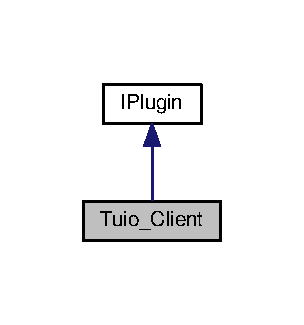
\includegraphics[width=146pt]{class_tuio___client__coll__graph}
\end{center}
\end{figure}
\subsection*{Public Member Functions}
\begin{DoxyCompactItemize}
\item 
void \hyperlink{class_tuio___client_a13aed5267c36dd0bc9b4dcf6939194d5}{Main} ()
\begin{DoxyCompactList}\small\item\em Main funcction of the plugin. \end{DoxyCompactList}\item 
bool \hyperlink{class_tuio___client_aef7de42628eef1f5c0fb3ff83b26de8b}{load\+Configuration} ()
\begin{DoxyCompactList}\small\item\em Load configuration. \end{DoxyCompactList}\item 
bool \hyperlink{class_tuio___client_a56700c6b7cf9447fde0e3828e90cd55f}{save\+Configuration} ()
\begin{DoxyCompactList}\small\item\em Save configuration. \end{DoxyCompactList}\item 
bool \hyperlink{class_tuio___client_a170015752bb0bb4c7815a08150a42620}{Initialize\+\_\+\+Output} ()
\begin{DoxyCompactList}\small\item\em Initialize Output variables for the plugin to publish. \end{DoxyCompactList}\item 
bool \hyperlink{class_tuio___client_a66bd1d9dc23405e7589d899ef6c5d892}{Initialize\+\_\+\+Input} ()
\begin{DoxyCompactList}\small\item\em Initialize Input variables for the plugin to publish. \end{DoxyCompactList}\item 
\mbox{\Hypertarget{class_tuio___client_a977ef88120a27438054a2638fb76af3c}\label{class_tuio___client_a977ef88120a27438054a2638fb76af3c}} 
void {\bfseries Init\+\_\+\+Joy} ()
\item 
void \hyperlink{class_tuio___client_ae326548bc87892e62dbe5f0a5a8b27cc}{run} ()
\begin{DoxyCompactList}\small\item\em Execute plugin. \end{DoxyCompactList}\item 
void \hyperlink{class_tuio___client_a2df126802294be8dc168c409af801779}{stop} ()
\begin{DoxyCompactList}\small\item\em Stop plugin. \end{DoxyCompactList}\end{DoxyCompactItemize}
\subsection*{Additional Inherited Members}


\subsection{Detailed Description}
\hyperlink{class_tuio___client}{Tuio\+\_\+\+Client} plugin. 

This plugin is a legacy wrapper that alows us to use Hocoma\textquotesingle{}s games with this architecture it writes output to a shared memory segment defined by hocoma that can not be changed \begin{DoxyAuthor}{Author}
Patrick Heyer, \href{mailto:patrickhey@prodigy.net.mx}{\tt patrickhey@prodigy.\+net.\+mx} 
\end{DoxyAuthor}
\begin{DoxyDate}{Date}
jul 13, 2014 
\end{DoxyDate}
\begin{DoxyVersion}{Version}
1.\+0 
\end{DoxyVersion}


Definition at line 100 of file Main.\+cpp.



\subsection{Member Function Documentation}
\mbox{\Hypertarget{class_tuio___client_a66bd1d9dc23405e7589d899ef6c5d892}\label{class_tuio___client_a66bd1d9dc23405e7589d899ef6c5d892}} 
\index{Tuio\+\_\+\+Client@{Tuio\+\_\+\+Client}!Initialize\+\_\+\+Input@{Initialize\+\_\+\+Input}}
\index{Initialize\+\_\+\+Input@{Initialize\+\_\+\+Input}!Tuio\+\_\+\+Client@{Tuio\+\_\+\+Client}}
\subsubsection{\texorpdfstring{Initialize\+\_\+\+Input()}{Initialize\_Input()}}
{\footnotesize\ttfamily bool Tuio\+\_\+\+Client\+::\+Initialize\+\_\+\+Input (\begin{DoxyParamCaption}{ }\end{DoxyParamCaption})\hspace{0.3cm}{\ttfamily [virtual]}}



Initialize Input variables for the plugin to publish. 

\begin{DoxyReturn}{Returns}
bool 
\end{DoxyReturn}


Implements \hyperlink{class_i_plugin_aa7c66743ad956d8ada57becee559af4d}{I\+Plugin}.



Definition at line 205 of file Main.\+cpp.


\begin{DoxyCode}
206 \{
207     RShoulder\_X=Shared\_Memory::getInstance().Register\_Double\_Input(\textcolor{stringliteral}{"RIGHT\_SHOULDER\_X"});
208     \textcolor{keywordflow}{return} \textcolor{keyword}{true};
209 \}
\end{DoxyCode}
\mbox{\Hypertarget{class_tuio___client_a170015752bb0bb4c7815a08150a42620}\label{class_tuio___client_a170015752bb0bb4c7815a08150a42620}} 
\index{Tuio\+\_\+\+Client@{Tuio\+\_\+\+Client}!Initialize\+\_\+\+Output@{Initialize\+\_\+\+Output}}
\index{Initialize\+\_\+\+Output@{Initialize\+\_\+\+Output}!Tuio\+\_\+\+Client@{Tuio\+\_\+\+Client}}
\subsubsection{\texorpdfstring{Initialize\+\_\+\+Output()}{Initialize\_Output()}}
{\footnotesize\ttfamily bool Tuio\+\_\+\+Client\+::\+Initialize\+\_\+\+Output (\begin{DoxyParamCaption}{ }\end{DoxyParamCaption})\hspace{0.3cm}{\ttfamily [virtual]}}



Initialize Output variables for the plugin to publish. 

\begin{DoxyReturn}{Returns}
bool 
\end{DoxyReturn}


Implements \hyperlink{class_i_plugin_a0b772513fc8c4ed01240e19c4bb84068}{I\+Plugin}.



Definition at line 198 of file Main.\+cpp.


\begin{DoxyCode}
199 \{
200     Shared\_Memory::getInstance().Register\_Output(\textcolor{stringliteral}{"TUIO\_0X"}, &X\_axis);
201     Shared\_Memory::getInstance().Register\_Output(\textcolor{stringliteral}{"TUIO\_0Y"}, &Y\_axis);
202     \textcolor{keywordflow}{return} \textcolor{keyword}{true};
203 \}
\end{DoxyCode}
\mbox{\Hypertarget{class_tuio___client_aef7de42628eef1f5c0fb3ff83b26de8b}\label{class_tuio___client_aef7de42628eef1f5c0fb3ff83b26de8b}} 
\index{Tuio\+\_\+\+Client@{Tuio\+\_\+\+Client}!load\+Configuration@{load\+Configuration}}
\index{load\+Configuration@{load\+Configuration}!Tuio\+\_\+\+Client@{Tuio\+\_\+\+Client}}
\subsubsection{\texorpdfstring{load\+Configuration()}{loadConfiguration()}}
{\footnotesize\ttfamily bool Tuio\+\_\+\+Client\+::load\+Configuration (\begin{DoxyParamCaption}{ }\end{DoxyParamCaption})\hspace{0.3cm}{\ttfamily [virtual]}}



Load configuration. 

The configuration can be loaded from file, or be hard coded into the plugin (not recomended), initialization of public and private variables should occur here

By default load\+Configuration is called during \hyperlink{class_plugin_manager_a956e653b7db36da9d034b4a93c8308d5}{Plugin\+Manager\+::\+Initialize()} by the plugin manager.

\begin{DoxyReturn}{Returns}
bool 
\end{DoxyReturn}


Implements \hyperlink{class_i_plugin_a418cff309436d3a15d9a4ce7369db6dd}{I\+Plugin}.



Definition at line 188 of file Main.\+cpp.


\begin{DoxyCode}
189 \{
190     \textcolor{keywordflow}{return} \textcolor{keyword}{true};
191 \}
\end{DoxyCode}
\mbox{\Hypertarget{class_tuio___client_a13aed5267c36dd0bc9b4dcf6939194d5}\label{class_tuio___client_a13aed5267c36dd0bc9b4dcf6939194d5}} 
\index{Tuio\+\_\+\+Client@{Tuio\+\_\+\+Client}!Main@{Main}}
\index{Main@{Main}!Tuio\+\_\+\+Client@{Tuio\+\_\+\+Client}}
\subsubsection{\texorpdfstring{Main()}{Main()}}
{\footnotesize\ttfamily void Tuio\+\_\+\+Client\+::\+Main (\begin{DoxyParamCaption}{ }\end{DoxyParamCaption})\hspace{0.3cm}{\ttfamily [virtual]}}



Main funcction of the plugin. 

Started in a new thread by the Run() funcction is the most importatn funcction of the plugin. Infinite loop (generaly a while(running) function that runs undefenitly in a read/process/write cicle). \begin{DoxyReturn}{Returns}
void 
\end{DoxyReturn}


Implements \hyperlink{class_i_plugin_ab5fdb3b0f7afdcee04324dca01766749}{I\+Plugin}.



Definition at line 152 of file Main.\+cpp.


\begin{DoxyCode}
153 \{
154     running=\textcolor{keyword}{true};
155     stoped=\textcolor{keyword}{false};
156 \textcolor{preprocessor}{#ifdef OPENGL\_GUI
}
157 
158     Gui::getInstance();
159     Tab *pluginTab;
160 
161     pluginTab = \textcolor{keyword}{new} Tab(\textcolor{stringliteral}{"Tuio\_Client"});
162     Gui::getInstance().setActiveTab(\textcolor{stringliteral}{"Tuio\_Client"});
163 
164 
165 
166 \textcolor{preprocessor}{#endif
}
167 \textcolor{keywordtype}{int} port = 3333;
168     
169 
170     TuioDump dump;
171     TuioClient client(port);
172     client.addTuioListener(&dump);
173     client.connect(\textcolor{keyword}{false});
174     
175 
176 
177     \textcolor{keywordflow}{while} (running)
178     \{
179 
180     \}
181     client.disconnect();
182 
183     stoped = \textcolor{keyword}{true};
184     \textcolor{keywordflow}{return};
185 
186 \}
\end{DoxyCode}
\mbox{\Hypertarget{class_tuio___client_ae326548bc87892e62dbe5f0a5a8b27cc}\label{class_tuio___client_ae326548bc87892e62dbe5f0a5a8b27cc}} 
\index{Tuio\+\_\+\+Client@{Tuio\+\_\+\+Client}!run@{run}}
\index{run@{run}!Tuio\+\_\+\+Client@{Tuio\+\_\+\+Client}}
\subsubsection{\texorpdfstring{run()}{run()}}
{\footnotesize\ttfamily void Tuio\+\_\+\+Client\+::run (\begin{DoxyParamCaption}{ }\end{DoxyParamCaption})\hspace{0.3cm}{\ttfamily [virtual]}}



Execute plugin. 

Starts a new thread and executes the plugins main() funcction. \begin{DoxyReturn}{Returns}
void 
\end{DoxyReturn}


Implements \hyperlink{class_i_plugin_a46b4ace767e77f9db9c9585e99c09039}{I\+Plugin}.



Definition at line 211 of file Main.\+cpp.



References I\+Plugin\+::\+Inc\+Wrapper().


\begin{DoxyCode}
212 \{
213     pthread\_create(&thread\_id, NULL, &\hyperlink{class_i_plugin_a62d22be2fdf66eb7f5c2f797f5f3d7f3}{IPlugin::IncWrapper}, \textcolor{keyword}{this});
214     running = \textcolor{keyword}{true};
215     stoped = \textcolor{keyword}{false};
216 \}
\end{DoxyCode}
\mbox{\Hypertarget{class_tuio___client_a56700c6b7cf9447fde0e3828e90cd55f}\label{class_tuio___client_a56700c6b7cf9447fde0e3828e90cd55f}} 
\index{Tuio\+\_\+\+Client@{Tuio\+\_\+\+Client}!save\+Configuration@{save\+Configuration}}
\index{save\+Configuration@{save\+Configuration}!Tuio\+\_\+\+Client@{Tuio\+\_\+\+Client}}
\subsubsection{\texorpdfstring{save\+Configuration()}{saveConfiguration()}}
{\footnotesize\ttfamily bool Tuio\+\_\+\+Client\+::save\+Configuration (\begin{DoxyParamCaption}{ }\end{DoxyParamCaption})\hspace{0.3cm}{\ttfamily [virtual]}}



Save configuration. 

The configuration should be saved to file, public and private variables that should be configured at startup should be saved.

By default save\+Configuration is called during \hyperlink{class_plugin_manager_ab651a05d6fcb92562807e9f5ecc30855}{Plugin\+Manager\+::\+Unload()} by the plugin manager.

\begin{DoxyReturn}{Returns}
bool 
\end{DoxyReturn}


Implements \hyperlink{class_i_plugin_a79b5c42b1c7b08257a6110b2091039bc}{I\+Plugin}.



Definition at line 193 of file Main.\+cpp.


\begin{DoxyCode}
194 \{
195     \textcolor{keywordflow}{return} \textcolor{keyword}{true};
196 \}
\end{DoxyCode}
\mbox{\Hypertarget{class_tuio___client_a2df126802294be8dc168c409af801779}\label{class_tuio___client_a2df126802294be8dc168c409af801779}} 
\index{Tuio\+\_\+\+Client@{Tuio\+\_\+\+Client}!stop@{stop}}
\index{stop@{stop}!Tuio\+\_\+\+Client@{Tuio\+\_\+\+Client}}
\subsubsection{\texorpdfstring{stop()}{stop()}}
{\footnotesize\ttfamily void Tuio\+\_\+\+Client\+::stop (\begin{DoxyParamCaption}{ }\end{DoxyParamCaption})\hspace{0.3cm}{\ttfamily [virtual]}}



Stop plugin. 

Stops the plugin \begin{DoxyReturn}{Returns}
void 
\end{DoxyReturn}


Implements \hyperlink{class_i_plugin_a86e523c283aec5c9fb21249a76e916ac}{I\+Plugin}.



Definition at line 218 of file Main.\+cpp.


\begin{DoxyCode}
219 \{
220     running = \textcolor{keyword}{false};
221 \}
\end{DoxyCode}


The documentation for this class was generated from the following file\+:\begin{DoxyCompactItemize}
\item 
/home/patrick/projects/\+Gesture\+\_\+\+Therapy\+\_\+\+Linux/src/\+Tuio\+\_\+\+Client/Main.\+cpp\end{DoxyCompactItemize}

\hypertarget{structuinput__event}{}\section{uinput\+\_\+event Struct Reference}
\label{structuinput__event}\index{uinput\+\_\+event@{uinput\+\_\+event}}
\subsection*{Public Attributes}
\begin{DoxyCompactItemize}
\item 
\mbox{\Hypertarget{structuinput__event_ae4282782ec7159f07b3ecec64a2fd4b2}\label{structuinput__event_ae4282782ec7159f07b3ecec64a2fd4b2}} 
struct timeval {\bfseries time}
\item 
\mbox{\Hypertarget{structuinput__event_a3042174c0b4572da8aab5d8de2e4ce90}\label{structuinput__event_a3042174c0b4572da8aab5d8de2e4ce90}} 
unsigned short {\bfseries type}
\item 
\mbox{\Hypertarget{structuinput__event_a04cfd9b357019858d2ed432c73d14481}\label{structuinput__event_a04cfd9b357019858d2ed432c73d14481}} 
unsigned short {\bfseries code}
\item 
\mbox{\Hypertarget{structuinput__event_ac3ec667a4c321cccb194773251d99ec4}\label{structuinput__event_ac3ec667a4c321cccb194773251d99ec4}} 
int {\bfseries value}
\end{DoxyCompactItemize}


\subsection{Detailed Description}


Definition at line 45 of file Joystick\+\_\+\+Writer.\+h.



The documentation for this struct was generated from the following file\+:\begin{DoxyCompactItemize}
\item 
/home/patrick/projects/\+Gesture\+\_\+\+Therapy\+\_\+\+Linux/src/\+Joystick\+\_\+\+Writer/Joystick\+\_\+\+Writer.\+h\end{DoxyCompactItemize}

\hypertarget{struct_x_input_joypad}{}\section{X\+Input\+Joypad Struct Reference}
\label{struct_x_input_joypad}\index{X\+Input\+Joypad@{X\+Input\+Joypad}}


Inheritance diagram for X\+Input\+Joypad\+:\nopagebreak
\begin{figure}[H]
\begin{center}
\leavevmode
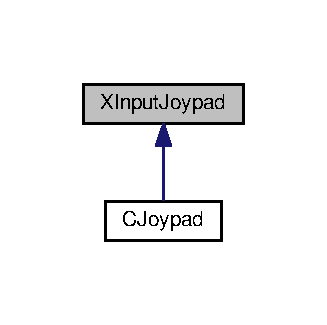
\includegraphics[width=157pt]{struct_x_input_joypad__inherit__graph}
\end{center}
\end{figure}
\subsection*{Public Types}
\begin{DoxyCompactItemize}
\item 
\mbox{\Hypertarget{struct_x_input_joypad_a3adfafecc1c0d3c88e354d90cc8cf5eb}\label{struct_x_input_joypad_a3adfafecc1c0d3c88e354d90cc8cf5eb}} 
enum \hyperlink{struct_x_input_joypad_a3adfafecc1c0d3c88e354d90cc8cf5eb}{e\+Axes} \{ \newline
{\bfseries X\+\_\+\+A\+X\+IS} = 0x00000001, 
{\bfseries Y\+\_\+\+A\+X\+IS} = 0x00000002, 
{\bfseries Z\+\_\+\+A\+X\+IS} = 0x00000004, 
{\bfseries X\+\_\+\+R\+O\+T\+\_\+\+A\+X\+IS} = 0x00000008, 
\newline
{\bfseries Y\+\_\+\+R\+O\+T\+\_\+\+A\+X\+IS} = 0x00000010, 
{\bfseries Z\+\_\+\+R\+O\+T\+\_\+\+A\+X\+IS} = 0x00000020, 
{\bfseries S\+L\+I\+D\+E\+R\+\_\+1} = 0x00000040, 
{\bfseries S\+L\+I\+D\+E\+R\+\_\+2} = 0x00000080, 
\newline
{\bfseries A\+X\+I\+S\+\_\+\+L\+A\+ST} = 0x\+F\+F\+F\+F\+F\+F\+FF
 \}\begin{DoxyCompactList}\small\item\em an enumeration to represent the various axes that may be available \end{DoxyCompactList}
\end{DoxyCompactItemize}
\subsection*{Public Member Functions}
\begin{DoxyCompactItemize}
\item 
\mbox{\Hypertarget{struct_x_input_joypad_a7119f927f05cfbeb65e3383fd81a1e1f}\label{struct_x_input_joypad_a7119f927f05cfbeb65e3383fd81a1e1f}} 
virtual bool {\bfseries Update} ()=0
\item 
\mbox{\Hypertarget{struct_x_input_joypad_a93c04a58a50c4c3b18d37d0716d526d6}\label{struct_x_input_joypad_a93c04a58a50c4c3b18d37d0716d526d6}} 
virtual const char $\ast$const {\bfseries Instance\+Name} () const =0
\item 
\mbox{\Hypertarget{struct_x_input_joypad_a7c56d532ce6a437a4caeca48c7daa466}\label{struct_x_input_joypad_a7c56d532ce6a437a4caeca48c7daa466}} 
virtual const char $\ast$const {\bfseries Product\+Name} () const =0
\item 
virtual const unsigned short \hyperlink{struct_x_input_joypad_a9bc1d9930ca27e815b05542a7fd38a39}{Num\+Buttons} () const =0
\item 
virtual const unsigned short \hyperlink{struct_x_input_joypad_a715b4a23b83fa39ca3940f4e2f45c852}{Num\+Povs} () const =0
\item 
virtual bool \hyperlink{struct_x_input_joypad_a9b5317808345c53bc0df5a3054dd0318}{HasX} () const =0
\item 
\mbox{\Hypertarget{struct_x_input_joypad_adc9941ccb63f0970f5a2224fb44fdcd0}\label{struct_x_input_joypad_adc9941ccb63f0970f5a2224fb44fdcd0}} 
virtual bool {\bfseries HasY} () const =0
\item 
\mbox{\Hypertarget{struct_x_input_joypad_af740d5b0bce33c49c4a4cb062d7df070}\label{struct_x_input_joypad_af740d5b0bce33c49c4a4cb062d7df070}} 
virtual bool {\bfseries HasZ} () const =0
\item 
\mbox{\Hypertarget{struct_x_input_joypad_af87200b7a9aa629bc3bca3376d125e73}\label{struct_x_input_joypad_af87200b7a9aa629bc3bca3376d125e73}} 
virtual bool {\bfseries Has\+Xrot} () const =0
\item 
\mbox{\Hypertarget{struct_x_input_joypad_a4a4f86be4f9cb79b5b6ae53fd07378b1}\label{struct_x_input_joypad_a4a4f86be4f9cb79b5b6ae53fd07378b1}} 
virtual bool {\bfseries Has\+Yrot} () const =0
\item 
\mbox{\Hypertarget{struct_x_input_joypad_a9d061e6be6ba35fbdb29a6ba11699184}\label{struct_x_input_joypad_a9d061e6be6ba35fbdb29a6ba11699184}} 
virtual bool {\bfseries Has\+Zrot} () const =0
\item 
\mbox{\Hypertarget{struct_x_input_joypad_a71ed4588a01d83d35d30f09746c93151}\label{struct_x_input_joypad_a71ed4588a01d83d35d30f09746c93151}} 
virtual bool {\bfseries Has\+Extra1} () const =0
\item 
\mbox{\Hypertarget{struct_x_input_joypad_adb69c84c61f7edc6de596a5bbe4306d6}\label{struct_x_input_joypad_adb69c84c61f7edc6de596a5bbe4306d6}} 
virtual bool {\bfseries Has\+Extra2} () const =0
\item 
virtual const bool \hyperlink{struct_x_input_joypad_a13cc187aae10747b0376cb1ed3710b5a}{Button} (const unsigned int \&i) const =0
\item 
\mbox{\Hypertarget{struct_x_input_joypad_af576c7afbf80332fd720903293ddc958}\label{struct_x_input_joypad_af576c7afbf80332fd720903293ddc958}} 
virtual const \hyperlink{_joypad_8h_a2a3e0cda5f1249bef6db47c5eb8e3813}{L\+O\+NG} \hyperlink{struct_x_input_joypad_af576c7afbf80332fd720903293ddc958}{Xaxis} () const =0
\begin{DoxyCompactList}\small\item\em X-\/axis, usually the left-\/right movement of a stick. \end{DoxyCompactList}\item 
\mbox{\Hypertarget{struct_x_input_joypad_af4753b9643cfa1f2c1cc71bca92c3be8}\label{struct_x_input_joypad_af4753b9643cfa1f2c1cc71bca92c3be8}} 
virtual const \hyperlink{_joypad_8h_a2a3e0cda5f1249bef6db47c5eb8e3813}{L\+O\+NG} \hyperlink{struct_x_input_joypad_af4753b9643cfa1f2c1cc71bca92c3be8}{Xvelocity} () const =0
\begin{DoxyCompactList}\small\item\em X-\/axis velocity. \end{DoxyCompactList}\item 
\mbox{\Hypertarget{struct_x_input_joypad_aa2e1a4b890b2bdeb94b5df3a6103cb3d}\label{struct_x_input_joypad_aa2e1a4b890b2bdeb94b5df3a6103cb3d}} 
virtual const \hyperlink{_joypad_8h_a2a3e0cda5f1249bef6db47c5eb8e3813}{L\+O\+NG} \hyperlink{struct_x_input_joypad_aa2e1a4b890b2bdeb94b5df3a6103cb3d}{Xacceleration} () const =0
\begin{DoxyCompactList}\small\item\em X-\/axis acceleration. \end{DoxyCompactList}\item 
\mbox{\Hypertarget{struct_x_input_joypad_a44f5f31e6f0f63e3708dd4f73fe385df}\label{struct_x_input_joypad_a44f5f31e6f0f63e3708dd4f73fe385df}} 
virtual const \hyperlink{_joypad_8h_a2a3e0cda5f1249bef6db47c5eb8e3813}{L\+O\+NG} \hyperlink{struct_x_input_joypad_a44f5f31e6f0f63e3708dd4f73fe385df}{Xforce} () const =0
\begin{DoxyCompactList}\small\item\em X-\/axis force. \end{DoxyCompactList}\item 
\mbox{\Hypertarget{struct_x_input_joypad_ac759aadee2870928828e8ab0454227f2}\label{struct_x_input_joypad_ac759aadee2870928828e8ab0454227f2}} 
virtual const \hyperlink{_joypad_8h_a2a3e0cda5f1249bef6db47c5eb8e3813}{L\+O\+NG} \hyperlink{struct_x_input_joypad_ac759aadee2870928828e8ab0454227f2}{Yaxis} () const =0
\begin{DoxyCompactList}\small\item\em Y-\/axis, usually the forward-\/backward movement of a stick. \end{DoxyCompactList}\item 
\mbox{\Hypertarget{struct_x_input_joypad_ac9a7c48ad012b41ed2113531cb0e6604}\label{struct_x_input_joypad_ac9a7c48ad012b41ed2113531cb0e6604}} 
virtual const \hyperlink{_joypad_8h_a2a3e0cda5f1249bef6db47c5eb8e3813}{L\+O\+NG} \hyperlink{struct_x_input_joypad_ac9a7c48ad012b41ed2113531cb0e6604}{Yvelocity} () const =0
\begin{DoxyCompactList}\small\item\em Y-\/axis velocity. \end{DoxyCompactList}\item 
\mbox{\Hypertarget{struct_x_input_joypad_a06c6ece1347b8bb7db762b0181fac206}\label{struct_x_input_joypad_a06c6ece1347b8bb7db762b0181fac206}} 
virtual const \hyperlink{_joypad_8h_a2a3e0cda5f1249bef6db47c5eb8e3813}{L\+O\+NG} \hyperlink{struct_x_input_joypad_a06c6ece1347b8bb7db762b0181fac206}{Yacceleration} () const =0
\begin{DoxyCompactList}\small\item\em Y-\/axis acceleration. \end{DoxyCompactList}\item 
\mbox{\Hypertarget{struct_x_input_joypad_a3365d3f59d8a45b96da53837872c09c6}\label{struct_x_input_joypad_a3365d3f59d8a45b96da53837872c09c6}} 
virtual const \hyperlink{_joypad_8h_a2a3e0cda5f1249bef6db47c5eb8e3813}{L\+O\+NG} \hyperlink{struct_x_input_joypad_a3365d3f59d8a45b96da53837872c09c6}{Yforce} () const =0
\begin{DoxyCompactList}\small\item\em Y-\/axis force. \end{DoxyCompactList}\item 
virtual const \hyperlink{_joypad_8h_a2a3e0cda5f1249bef6db47c5eb8e3813}{L\+O\+NG} \hyperlink{struct_x_input_joypad_af4bfca4d8f22808a92a0ae26468cdedc}{Zaxis} () const =0
\item 
\mbox{\Hypertarget{struct_x_input_joypad_a324d7b6c76e29d4dec9f1ecfbf771243}\label{struct_x_input_joypad_a324d7b6c76e29d4dec9f1ecfbf771243}} 
virtual const \hyperlink{_joypad_8h_a2a3e0cda5f1249bef6db47c5eb8e3813}{L\+O\+NG} \hyperlink{struct_x_input_joypad_a324d7b6c76e29d4dec9f1ecfbf771243}{Zvelocity} () const =0
\begin{DoxyCompactList}\small\item\em Z-\/axis velocity. \end{DoxyCompactList}\item 
\mbox{\Hypertarget{struct_x_input_joypad_ac6f8ddb5e87a0c30e6c454f1f2ff506b}\label{struct_x_input_joypad_ac6f8ddb5e87a0c30e6c454f1f2ff506b}} 
virtual const \hyperlink{_joypad_8h_a2a3e0cda5f1249bef6db47c5eb8e3813}{L\+O\+NG} \hyperlink{struct_x_input_joypad_ac6f8ddb5e87a0c30e6c454f1f2ff506b}{Zacceleration} () const =0
\begin{DoxyCompactList}\small\item\em Z-\/axis acceleration. \end{DoxyCompactList}\item 
\mbox{\Hypertarget{struct_x_input_joypad_ad27b9f26025b9c2a5ffc7c12ec230d18}\label{struct_x_input_joypad_ad27b9f26025b9c2a5ffc7c12ec230d18}} 
virtual const \hyperlink{_joypad_8h_a2a3e0cda5f1249bef6db47c5eb8e3813}{L\+O\+NG} \hyperlink{struct_x_input_joypad_ad27b9f26025b9c2a5ffc7c12ec230d18}{Zforce} () const =0
\begin{DoxyCompactList}\small\item\em Z-\/axis force. \end{DoxyCompactList}\item 
\mbox{\Hypertarget{struct_x_input_joypad_a7142a1f6548cc59553846ca7e9889ef6}\label{struct_x_input_joypad_a7142a1f6548cc59553846ca7e9889ef6}} 
virtual const \hyperlink{_joypad_8h_a2a3e0cda5f1249bef6db47c5eb8e3813}{L\+O\+NG} \hyperlink{struct_x_input_joypad_a7142a1f6548cc59553846ca7e9889ef6}{Xrot} () const =0
\begin{DoxyCompactList}\small\item\em X-\/axis rotation. If the joystick does not have this axis, the value is 0. \end{DoxyCompactList}\item 
\mbox{\Hypertarget{struct_x_input_joypad_ad6bcc1e11d6acbd06ebf5829be849eed}\label{struct_x_input_joypad_ad6bcc1e11d6acbd06ebf5829be849eed}} 
virtual const \hyperlink{_joypad_8h_a2a3e0cda5f1249bef6db47c5eb8e3813}{L\+O\+NG} \hyperlink{struct_x_input_joypad_ad6bcc1e11d6acbd06ebf5829be849eed}{Xrot\+Velocity} () const =0
\begin{DoxyCompactList}\small\item\em X-\/axis angular velocity. \end{DoxyCompactList}\item 
\mbox{\Hypertarget{struct_x_input_joypad_a7e10a4c04604b17b8148e547625d840d}\label{struct_x_input_joypad_a7e10a4c04604b17b8148e547625d840d}} 
virtual const \hyperlink{_joypad_8h_a2a3e0cda5f1249bef6db47c5eb8e3813}{L\+O\+NG} \hyperlink{struct_x_input_joypad_a7e10a4c04604b17b8148e547625d840d}{Xrot\+Acceleration} () const =0
\begin{DoxyCompactList}\small\item\em X-\/axis angular acceleration. \end{DoxyCompactList}\item 
\mbox{\Hypertarget{struct_x_input_joypad_a4499b53bed5f47866f2afb7f8ff4fd90}\label{struct_x_input_joypad_a4499b53bed5f47866f2afb7f8ff4fd90}} 
virtual const \hyperlink{_joypad_8h_a2a3e0cda5f1249bef6db47c5eb8e3813}{L\+O\+NG} \hyperlink{struct_x_input_joypad_a4499b53bed5f47866f2afb7f8ff4fd90}{Xrot\+Force} () const =0
\begin{DoxyCompactList}\small\item\em X-\/axis torque. \end{DoxyCompactList}\item 
\mbox{\Hypertarget{struct_x_input_joypad_a20614fa56d86ebf80bd376e382da3967}\label{struct_x_input_joypad_a20614fa56d86ebf80bd376e382da3967}} 
virtual const \hyperlink{_joypad_8h_a2a3e0cda5f1249bef6db47c5eb8e3813}{L\+O\+NG} \hyperlink{struct_x_input_joypad_a20614fa56d86ebf80bd376e382da3967}{Yrot} () const =0
\begin{DoxyCompactList}\small\item\em Y-\/axis rotation. If the joystick does not have this axis, the value is 0. \end{DoxyCompactList}\item 
\mbox{\Hypertarget{struct_x_input_joypad_af59eac449d0f28bbe306d0a2ffbfa1d9}\label{struct_x_input_joypad_af59eac449d0f28bbe306d0a2ffbfa1d9}} 
virtual const \hyperlink{_joypad_8h_a2a3e0cda5f1249bef6db47c5eb8e3813}{L\+O\+NG} \hyperlink{struct_x_input_joypad_af59eac449d0f28bbe306d0a2ffbfa1d9}{Yrot\+Velocity} () const =0
\begin{DoxyCompactList}\small\item\em Y-\/axis angular velocity. \end{DoxyCompactList}\item 
\mbox{\Hypertarget{struct_x_input_joypad_a429b94f4163b681812ed8ec3e0deb57f}\label{struct_x_input_joypad_a429b94f4163b681812ed8ec3e0deb57f}} 
virtual const \hyperlink{_joypad_8h_a2a3e0cda5f1249bef6db47c5eb8e3813}{L\+O\+NG} \hyperlink{struct_x_input_joypad_a429b94f4163b681812ed8ec3e0deb57f}{Yrot\+Acceleration} () const =0
\begin{DoxyCompactList}\small\item\em Y-\/axis angular acceleration. \end{DoxyCompactList}\item 
\mbox{\Hypertarget{struct_x_input_joypad_ab8430f97568768c719350987246876e4}\label{struct_x_input_joypad_ab8430f97568768c719350987246876e4}} 
virtual const \hyperlink{_joypad_8h_a2a3e0cda5f1249bef6db47c5eb8e3813}{L\+O\+NG} \hyperlink{struct_x_input_joypad_ab8430f97568768c719350987246876e4}{Yrot\+Force} () const =0
\begin{DoxyCompactList}\small\item\em Y-\/axis torque. \end{DoxyCompactList}\item 
virtual const \hyperlink{_joypad_8h_a2a3e0cda5f1249bef6db47c5eb8e3813}{L\+O\+NG} \hyperlink{struct_x_input_joypad_a4319cae362154a8e069ebe290db8239b}{Zrot} () const =0
\item 
\mbox{\Hypertarget{struct_x_input_joypad_acfaa90edbc89522947d169fdd89d82a8}\label{struct_x_input_joypad_acfaa90edbc89522947d169fdd89d82a8}} 
virtual const \hyperlink{_joypad_8h_a2a3e0cda5f1249bef6db47c5eb8e3813}{L\+O\+NG} \hyperlink{struct_x_input_joypad_acfaa90edbc89522947d169fdd89d82a8}{Zrot\+Velocity} () const =0
\begin{DoxyCompactList}\small\item\em Z-\/axis angular velocity. . \end{DoxyCompactList}\item 
\mbox{\Hypertarget{struct_x_input_joypad_a17a9b04c995dce9a76925cd1189facc1}\label{struct_x_input_joypad_a17a9b04c995dce9a76925cd1189facc1}} 
virtual const \hyperlink{_joypad_8h_a2a3e0cda5f1249bef6db47c5eb8e3813}{L\+O\+NG} \hyperlink{struct_x_input_joypad_a17a9b04c995dce9a76925cd1189facc1}{Zrot\+Acceleration} () const =0
\begin{DoxyCompactList}\small\item\em Z-\/axis angular acceleration. \end{DoxyCompactList}\item 
\mbox{\Hypertarget{struct_x_input_joypad_ab831c12b47291cc3d3892ed56c1f880e}\label{struct_x_input_joypad_ab831c12b47291cc3d3892ed56c1f880e}} 
virtual const \hyperlink{_joypad_8h_a2a3e0cda5f1249bef6db47c5eb8e3813}{L\+O\+NG} \hyperlink{struct_x_input_joypad_ab831c12b47291cc3d3892ed56c1f880e}{Zrot\+Force} () const =0
\begin{DoxyCompactList}\small\item\em Z-\/axis torque. \end{DoxyCompactList}\item 
virtual const \hyperlink{_joypad_8h_a2a3e0cda5f1249bef6db47c5eb8e3813}{L\+O\+NG} \hyperlink{struct_x_input_joypad_a074ad76f1e54b559fcee6606049bb6b7}{Extra\+Axes} (const unsigned int \&i) const =0
\item 
\mbox{\Hypertarget{struct_x_input_joypad_aabd7d5d90730169be8278036de089e49}\label{struct_x_input_joypad_aabd7d5d90730169be8278036de089e49}} 
virtual const \hyperlink{_joypad_8h_a2a3e0cda5f1249bef6db47c5eb8e3813}{L\+O\+NG} {\bfseries Extra\+Velocities} (const unsigned int \&i) const =0
\item 
\mbox{\Hypertarget{struct_x_input_joypad_aa36c5b3fcfeab916dcd011e8f0e1f8bd}\label{struct_x_input_joypad_aa36c5b3fcfeab916dcd011e8f0e1f8bd}} 
virtual const \hyperlink{_joypad_8h_a2a3e0cda5f1249bef6db47c5eb8e3813}{L\+O\+NG} {\bfseries Extra\+Accelerations} (const unsigned int \&i) const =0
\item 
\mbox{\Hypertarget{struct_x_input_joypad_aabb3c119fb0512f326036c8d0cee4bf2}\label{struct_x_input_joypad_aabb3c119fb0512f326036c8d0cee4bf2}} 
virtual const \hyperlink{_joypad_8h_a2a3e0cda5f1249bef6db47c5eb8e3813}{L\+O\+NG} {\bfseries Extra\+Forces} (const unsigned int \&i) const =0
\item 
virtual const D\+W\+O\+RD \hyperlink{struct_x_input_joypad_a2f270f296bcaf98089ab23f74a6e9937}{P\+OV} (const unsigned int \&i) const =0
\end{DoxyCompactItemize}


\subsection{Detailed Description}


Definition at line 50 of file Joypad.\+h.



\subsection{Member Function Documentation}
\mbox{\Hypertarget{struct_x_input_joypad_a13cc187aae10747b0376cb1ed3710b5a}\label{struct_x_input_joypad_a13cc187aae10747b0376cb1ed3710b5a}} 
\index{X\+Input\+Joypad@{X\+Input\+Joypad}!Button@{Button}}
\index{Button@{Button}!X\+Input\+Joypad@{X\+Input\+Joypad}}
\subsubsection{\texorpdfstring{Button()}{Button()}}
{\footnotesize\ttfamily virtual const bool X\+Input\+Joypad\+::\+Button (\begin{DoxyParamCaption}\item[{const unsigned int \&}]{i }\end{DoxyParamCaption}) const\hspace{0.3cm}{\ttfamily [pure virtual]}}

Array of buttons. The high-\/order bit of the byte is set if the corresponding button is down, and clear if the button is up or does not exist. 

Implemented in \hyperlink{class_c_joypad_a0125d648a2866c9524e70e3ddeb8b675}{C\+Joypad}.

\mbox{\Hypertarget{struct_x_input_joypad_a074ad76f1e54b559fcee6606049bb6b7}\label{struct_x_input_joypad_a074ad76f1e54b559fcee6606049bb6b7}} 
\index{X\+Input\+Joypad@{X\+Input\+Joypad}!Extra\+Axes@{Extra\+Axes}}
\index{Extra\+Axes@{Extra\+Axes}!X\+Input\+Joypad@{X\+Input\+Joypad}}
\subsubsection{\texorpdfstring{Extra\+Axes()}{ExtraAxes()}}
{\footnotesize\ttfamily virtual const \hyperlink{_joypad_8h_a2a3e0cda5f1249bef6db47c5eb8e3813}{L\+O\+NG} X\+Input\+Joypad\+::\+Extra\+Axes (\begin{DoxyParamCaption}\item[{const unsigned int \&}]{i }\end{DoxyParamCaption}) const\hspace{0.3cm}{\ttfamily [pure virtual]}}

Two additional axis values (formerly called the u-\/axis and v-\/axis) whose semantics depend on the joystick. Use the I\+Direct\+Input\+Device8\+::\+Get\+Object\+Info method to obtain semantic information about these values. 

Implemented in \hyperlink{class_c_joypad_ac94bd5a534d97f4c82456397e9a01b1c}{C\+Joypad}.

\mbox{\Hypertarget{struct_x_input_joypad_a9b5317808345c53bc0df5a3054dd0318}\label{struct_x_input_joypad_a9b5317808345c53bc0df5a3054dd0318}} 
\index{X\+Input\+Joypad@{X\+Input\+Joypad}!HasX@{HasX}}
\index{HasX@{HasX}!X\+Input\+Joypad@{X\+Input\+Joypad}}
\subsubsection{\texorpdfstring{Has\+X()}{HasX()}}
{\footnotesize\ttfamily virtual bool X\+Input\+Joypad\+::\+HasX (\begin{DoxyParamCaption}{ }\end{DoxyParamCaption}) const\hspace{0.3cm}{\ttfamily [pure virtual]}}

the following functions allow you to check to see if the specified axis is available on the joypad. 

Implemented in \hyperlink{class_c_joypad_aad2ba56e14016ef5cd7120b6097caa8c}{C\+Joypad}.

\mbox{\Hypertarget{struct_x_input_joypad_a9bc1d9930ca27e815b05542a7fd38a39}\label{struct_x_input_joypad_a9bc1d9930ca27e815b05542a7fd38a39}} 
\index{X\+Input\+Joypad@{X\+Input\+Joypad}!Num\+Buttons@{Num\+Buttons}}
\index{Num\+Buttons@{Num\+Buttons}!X\+Input\+Joypad@{X\+Input\+Joypad}}
\subsubsection{\texorpdfstring{Num\+Buttons()}{NumButtons()}}
{\footnotesize\ttfamily virtual const unsigned short X\+Input\+Joypad\+::\+Num\+Buttons (\begin{DoxyParamCaption}{ }\end{DoxyParamCaption}) const\hspace{0.3cm}{\ttfamily [pure virtual]}}

this function returns the number of buttons available on the joypad 

Implemented in \hyperlink{class_c_joypad_ab3a3683d1b12e2071af4751afc2d749c}{C\+Joypad}.

\mbox{\Hypertarget{struct_x_input_joypad_a715b4a23b83fa39ca3940f4e2f45c852}\label{struct_x_input_joypad_a715b4a23b83fa39ca3940f4e2f45c852}} 
\index{X\+Input\+Joypad@{X\+Input\+Joypad}!Num\+Povs@{Num\+Povs}}
\index{Num\+Povs@{Num\+Povs}!X\+Input\+Joypad@{X\+Input\+Joypad}}
\subsubsection{\texorpdfstring{Num\+Povs()}{NumPovs()}}
{\footnotesize\ttfamily virtual const unsigned short X\+Input\+Joypad\+::\+Num\+Povs (\begin{DoxyParamCaption}{ }\end{DoxyParamCaption}) const\hspace{0.3cm}{\ttfamily [pure virtual]}}

this function returns the number of buttons available on the joypad 

Implemented in \hyperlink{class_c_joypad_af40e2d5725c3e4d6bdc772e24bb52dca}{C\+Joypad}.

\mbox{\Hypertarget{struct_x_input_joypad_a2f270f296bcaf98089ab23f74a6e9937}\label{struct_x_input_joypad_a2f270f296bcaf98089ab23f74a6e9937}} 
\index{X\+Input\+Joypad@{X\+Input\+Joypad}!P\+OV@{P\+OV}}
\index{P\+OV@{P\+OV}!X\+Input\+Joypad@{X\+Input\+Joypad}}
\subsubsection{\texorpdfstring{P\+O\+V()}{POV()}}
{\footnotesize\ttfamily virtual const D\+W\+O\+RD X\+Input\+Joypad\+::\+P\+OV (\begin{DoxyParamCaption}\item[{const unsigned int \&}]{i }\end{DoxyParamCaption}) const\hspace{0.3cm}{\ttfamily [pure virtual]}}

Direction controllers, such as point-\/of-\/view hats. The position is indicated in hundredths of a degree clockwise from north (away from the user). The center position is normally reported as -\/1; but see Remarks. For indicators that have only five positions, the value for a controller is -\/1, 0, 9,000, 18,000, or 27,000. 

Implemented in \hyperlink{class_c_joypad_a52dad2bae4ae8ef1574d963bdd4c1a5d}{C\+Joypad}.

\mbox{\Hypertarget{struct_x_input_joypad_af4bfca4d8f22808a92a0ae26468cdedc}\label{struct_x_input_joypad_af4bfca4d8f22808a92a0ae26468cdedc}} 
\index{X\+Input\+Joypad@{X\+Input\+Joypad}!Zaxis@{Zaxis}}
\index{Zaxis@{Zaxis}!X\+Input\+Joypad@{X\+Input\+Joypad}}
\subsubsection{\texorpdfstring{Zaxis()}{Zaxis()}}
{\footnotesize\ttfamily virtual const \hyperlink{_joypad_8h_a2a3e0cda5f1249bef6db47c5eb8e3813}{L\+O\+NG} X\+Input\+Joypad\+::\+Zaxis (\begin{DoxyParamCaption}{ }\end{DoxyParamCaption}) const\hspace{0.3cm}{\ttfamily [pure virtual]}}

Z-\/axis, often the throttle control. If the joystick does not have this axis, the value is 0. 

Implemented in \hyperlink{class_c_joypad_a1ab390e90331bc036447eb4fc477e796}{C\+Joypad}.

\mbox{\Hypertarget{struct_x_input_joypad_a4319cae362154a8e069ebe290db8239b}\label{struct_x_input_joypad_a4319cae362154a8e069ebe290db8239b}} 
\index{X\+Input\+Joypad@{X\+Input\+Joypad}!Zrot@{Zrot}}
\index{Zrot@{Zrot}!X\+Input\+Joypad@{X\+Input\+Joypad}}
\subsubsection{\texorpdfstring{Zrot()}{Zrot()}}
{\footnotesize\ttfamily virtual const \hyperlink{_joypad_8h_a2a3e0cda5f1249bef6db47c5eb8e3813}{L\+O\+NG} X\+Input\+Joypad\+::\+Zrot (\begin{DoxyParamCaption}{ }\end{DoxyParamCaption}) const\hspace{0.3cm}{\ttfamily [pure virtual]}}

Z-\/axis rotation (often called the rudder). If the joystick does not have this axis, the value is 0. 

Implemented in \hyperlink{class_c_joypad_a4cd374af62d1380af4f92156503330a7}{C\+Joypad}.



The documentation for this struct was generated from the following file\+:\begin{DoxyCompactItemize}
\item 
/home/patrick/projects/\+Gesture\+\_\+\+Therapy\+\_\+\+Linux/src/\+Joystick\+\_\+\+Reader/\hyperlink{_joypad_8h}{Joypad.\+h}\end{DoxyCompactItemize}

\chapter{File Documentation}
\hypertarget{_joypad_8h}{}\section{/home/patrick/projects/\+Gesture\+\_\+\+Therapy\+\_\+\+Linux/src/\+Joystick\+\_\+\+Reader/\+Joypad.h File Reference}
\label{_joypad_8h}\index{/home/patrick/projects/\+Gesture\+\_\+\+Therapy\+\_\+\+Linux/src/\+Joystick\+\_\+\+Reader/\+Joypad.\+h@{/home/patrick/projects/\+Gesture\+\_\+\+Therapy\+\_\+\+Linux/src/\+Joystick\+\_\+\+Reader/\+Joypad.\+h}}


This file provides a generic cross platform joypad interface for Win32 \& Linux. Generally the linux implimentation is not as cool as using DirectX, you only really get hold of the values. Using force feedback is beyond Linux at the moment. Oh well...  


{\ttfamily \#include $<$string$>$}\newline
{\ttfamily \#include $<$iostream$>$}\newline
Include dependency graph for Joypad.\+h\+:\nopagebreak
\begin{figure}[H]
\begin{center}
\leavevmode
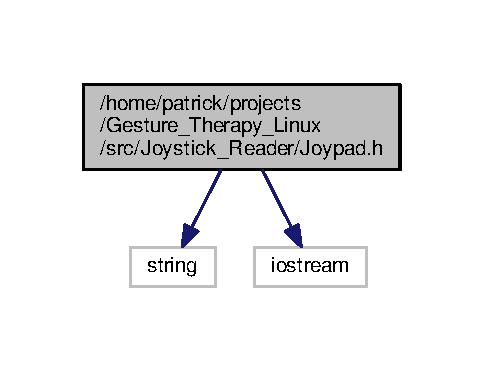
\includegraphics[width=232pt]{_joypad_8h__incl}
\end{center}
\end{figure}
This graph shows which files directly or indirectly include this file\+:\nopagebreak
\begin{figure}[H]
\begin{center}
\leavevmode
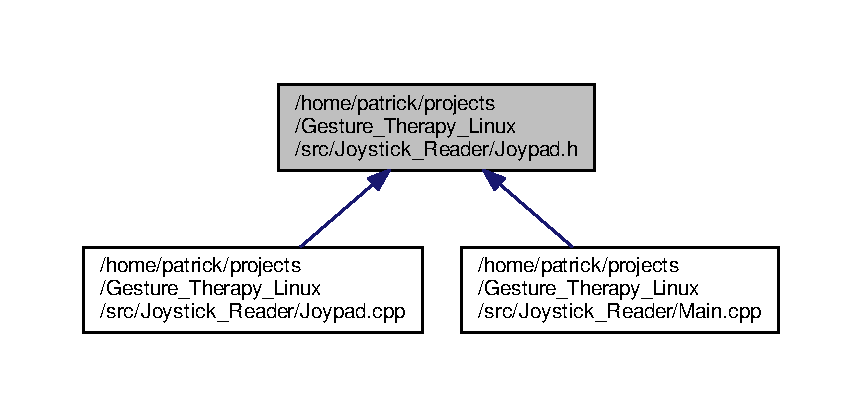
\includegraphics[width=350pt]{_joypad_8h__dep__incl}
\end{center}
\end{figure}
\subsection*{Classes}
\begin{DoxyCompactItemize}
\item 
struct \hyperlink{struct_x_input_joypad}{X\+Input\+Joypad}
\item 
class \hyperlink{class_c_joypad}{C\+Joypad}
\end{DoxyCompactItemize}
\subsection*{Typedefs}
\begin{DoxyCompactItemize}
\item 
\mbox{\Hypertarget{_joypad_8h_a2a3e0cda5f1249bef6db47c5eb8e3813}\label{_joypad_8h_a2a3e0cda5f1249bef6db47c5eb8e3813}} 
typedef long \hyperlink{_joypad_8h_a2a3e0cda5f1249bef6db47c5eb8e3813}{L\+O\+NG}
\begin{DoxyCompactList}\small\item\em make sure D\+W\+O\+RD and L\+O\+NG and defined in linux land \end{DoxyCompactList}\item 
\mbox{\Hypertarget{_joypad_8h_ad342ac907eb044443153a22f964bf0af}\label{_joypad_8h_ad342ac907eb044443153a22f964bf0af}} 
typedef unsigned long {\bfseries D\+W\+O\+RD}
\end{DoxyCompactItemize}
\subsection*{Functions}
\begin{DoxyCompactItemize}
\item 
\mbox{\Hypertarget{_joypad_8h_afa3d6b1e053da0648e2fdf9a519c3e43}\label{_joypad_8h_afa3d6b1e053da0648e2fdf9a519c3e43}} 
unsigned int \hyperlink{_joypad_8h_afa3d6b1e053da0648e2fdf9a519c3e43}{Num\+Joypads} ()
\begin{DoxyCompactList}\small\item\em This function returns the number of working joypads attached to the computer. \end{DoxyCompactList}\item 
\mbox{\Hypertarget{_joypad_8h_ae9a61e670cc624c9b5e1d365c157cd53}\label{_joypad_8h_ae9a61e670cc624c9b5e1d365c157cd53}} 
\hyperlink{struct_x_input_joypad}{X\+Input\+Joypad} $\ast$ \hyperlink{_joypad_8h_ae9a61e670cc624c9b5e1d365c157cd53}{Get\+Joypad} (const unsigned int=0)
\begin{DoxyCompactList}\small\item\em This function returns a pointer to the requested Joypad or N\+U\+LL if no joypad is available. \end{DoxyCompactList}\item 
void \hyperlink{_joypad_8h_abdb51d74a8798e93a46d3149db9d387b}{Free\+Input} ()
\begin{DoxyCompactList}\small\item\em This function is called to destroy the input at the end of the game. \end{DoxyCompactList}\item 
bool \hyperlink{_joypad_8h_ab38988ebf6ab3808447c491d4f5874e0}{Init\+Input} ()
\begin{DoxyCompactList}\small\item\em This function can be used to initialise the joypad lib. \end{DoxyCompactList}\item 
bool \hyperlink{_joypad_8h_a4d5dc1be49e0a6ddee2df5035bc2b56f}{Update\+Input\+State} ()
\begin{DoxyCompactList}\small\item\em You should call this to update the state of the joypad. \end{DoxyCompactList}\end{DoxyCompactItemize}


\subsection{Detailed Description}
This file provides a generic cross platform joypad interface for Win32 \& Linux. Generally the linux implimentation is not as cool as using DirectX, you only really get hold of the values. Using force feedback is beyond Linux at the moment. Oh well... 

\begin{DoxyAuthor}{Author}
Rob Bateman 
\end{DoxyAuthor}
\begin{DoxyDate}{Date}
12-\/jan-\/2004 
\end{DoxyDate}


\subsection{Function Documentation}
\mbox{\Hypertarget{_joypad_8h_abdb51d74a8798e93a46d3149db9d387b}\label{_joypad_8h_abdb51d74a8798e93a46d3149db9d387b}} 
\index{Joypad.\+h@{Joypad.\+h}!Free\+Input@{Free\+Input}}
\index{Free\+Input@{Free\+Input}!Joypad.\+h@{Joypad.\+h}}
\subsubsection{\texorpdfstring{Free\+Input()}{FreeInput()}}
{\footnotesize\ttfamily void Free\+Input (\begin{DoxyParamCaption}{ }\end{DoxyParamCaption})}



This function is called to destroy the input at the end of the game. 

Cleans up Direct Input.

This function is called to destroy the input at the end of the game. 

Definition at line 405 of file Joypad.\+cpp.



Referenced by C\+Joypad\+::\+P\+O\+V().


\begin{DoxyCode}
406 \{
407     std::vector< XInputJoypad* >::iterator it = g\_aJoypads.begin();
408     \textcolor{keywordflow}{for}( ; it != g\_aJoypads.end(); ++it )
409     \{
410         \textcolor{keyword}{delete} (*it);
411     \}
412     g\_aJoypads.resize(0);
413 \}
\end{DoxyCode}
\mbox{\Hypertarget{_joypad_8h_ab38988ebf6ab3808447c491d4f5874e0}\label{_joypad_8h_ab38988ebf6ab3808447c491d4f5874e0}} 
\index{Joypad.\+h@{Joypad.\+h}!Init\+Input@{Init\+Input}}
\index{Init\+Input@{Init\+Input}!Joypad.\+h@{Joypad.\+h}}
\subsubsection{\texorpdfstring{Init\+Input()}{InitInput()}}
{\footnotesize\ttfamily bool Init\+Input (\begin{DoxyParamCaption}{ }\end{DoxyParamCaption})}



This function can be used to initialise the joypad lib. 

Initialize the Direct\+Input variables.

\begin{DoxyReturn}{Returns}
true if OK, false if it fails
\end{DoxyReturn}
This function can be used to initialise the joypad lib.

\begin{DoxyReturn}{Returns}
true if OK 
\end{DoxyReturn}


Definition at line 383 of file Joypad.\+cpp.



Referenced by C\+Joypad\+::\+P\+O\+V().


\begin{DoxyCode}
384 \{
385     \textcolor{keywordtype}{bool} ret=\textcolor{keyword}{false};
386     \textcolor{keywordtype}{int} fd;
387     \textcolor{keywordflow}{if} ( (fd = open(\textcolor{stringliteral}{"/dev/input/js0"}, O\_RDONLY)) > 0 ) 
388     \{
389         \hyperlink{class_c_joypad}{CJoypad}* ptr = \textcolor{keyword}{new} \hyperlink{class_c_joypad}{CJoypad};
390         ioctl(fd, JSIOCGVERSION, &ptr->version);
391         ioctl(fd, JSIOCGAXES, &ptr->m\_iAxes);
392         ioctl(fd, JSIOCGBUTTONS, &ptr->m\_nButtons);
393         ioctl(fd, JSIOCGNAME(NAME\_LENGTH), ptr->name);
394         fcntl(fd, F\_SETFL, O\_NONBLOCK);
395         ptr->fd = fd;
396         g\_aJoypads.push\_back(ptr);
397         ret=\textcolor{keyword}{true};
398     \}
399     \textcolor{keywordflow}{return} ret;
400 \}
\end{DoxyCode}
\mbox{\Hypertarget{_joypad_8h_a4d5dc1be49e0a6ddee2df5035bc2b56f}\label{_joypad_8h_a4d5dc1be49e0a6ddee2df5035bc2b56f}} 
\index{Joypad.\+h@{Joypad.\+h}!Update\+Input\+State@{Update\+Input\+State}}
\index{Update\+Input\+State@{Update\+Input\+State}!Joypad.\+h@{Joypad.\+h}}
\subsubsection{\texorpdfstring{Update\+Input\+State()}{UpdateInputState()}}
{\footnotesize\ttfamily bool Update\+Input\+State (\begin{DoxyParamCaption}{ }\end{DoxyParamCaption})}



You should call this to update the state of the joypad. 

\begin{DoxyReturn}{Returns}
true if OK. 
\end{DoxyReturn}


Definition at line 370 of file Joypad.\+cpp.



Referenced by C\+Joypad\+::\+P\+O\+V().


\begin{DoxyCode}
371 \{
372     std::vector< XInputJoypad* >::iterator it = g\_aJoypads.begin();
373     \textcolor{keywordflow}{for}( ; it != g\_aJoypads.end(); ++it )
374     \{
375         (*it)->Update();
376     \}
377 \}
\end{DoxyCode}

\hypertarget{coreapi_8h}{}\section{/home/patrick/projects/\+Gesture\+\_\+\+Therapy\+\_\+\+Linux/src/\+Plugin\+\_\+\+A\+P\+I/coreapi.h File Reference}
\label{coreapi_8h}\index{/home/patrick/projects/\+Gesture\+\_\+\+Therapy\+\_\+\+Linux/src/\+Plugin\+\_\+\+A\+P\+I/coreapi.\+h@{/home/patrick/projects/\+Gesture\+\_\+\+Therapy\+\_\+\+Linux/src/\+Plugin\+\_\+\+A\+P\+I/coreapi.\+h}}


A factory object to create Renderer instances.  


{\ttfamily \#include \char`\"{}defines.\+h\char`\"{}}\newline
{\ttfamily \#include \char`\"{}plugin.\+h\char`\"{}}\newline
{\ttfamily \#include $<$string$>$}\newline
{\ttfamily \#include $<$map$>$}\newline
Include dependency graph for coreapi.\+h\+:\nopagebreak
\begin{figure}[H]
\begin{center}
\leavevmode
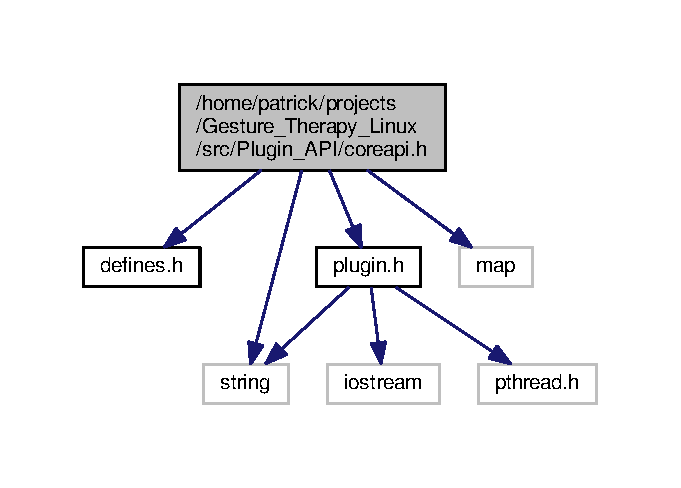
\includegraphics[width=327pt]{coreapi_8h__incl}
\end{center}
\end{figure}
This graph shows which files directly or indirectly include this file\+:\nopagebreak
\begin{figure}[H]
\begin{center}
\leavevmode
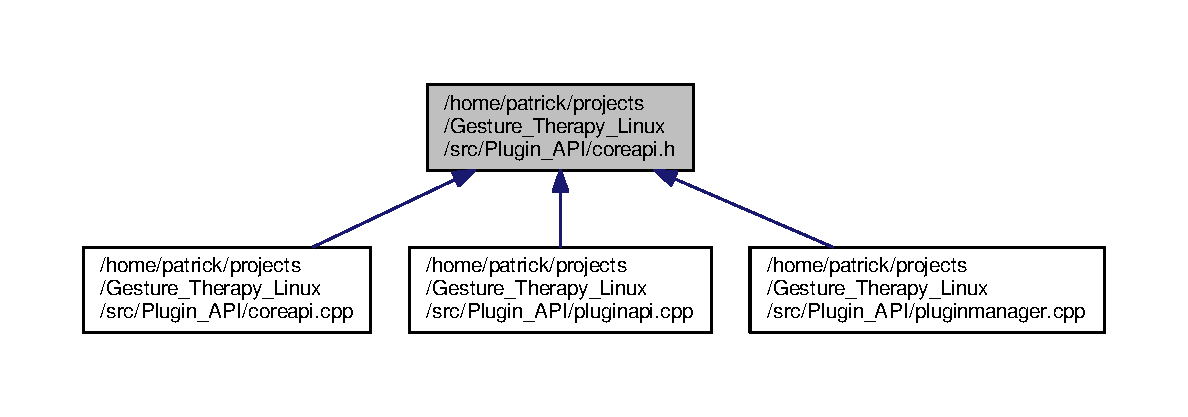
\includegraphics[width=350pt]{coreapi_8h__dep__incl}
\end{center}
\end{figure}
\subsection*{Classes}
\begin{DoxyCompactItemize}
\item 
class \hyperlink{class_plugin_factory}{Plugin\+Factory}
\end{DoxyCompactItemize}


\subsection{Detailed Description}
A factory object to create Renderer instances. 

\begin{DoxyAuthor}{Author}
Patrick Heyer \href{mailto:patrickhey@prodigy.net.mx}{\tt patrickhey@prodigy.\+net.\+mx} 
\end{DoxyAuthor}

\hypertarget{defines_8h}{}\section{/home/patrick/projects/\+Gesture\+\_\+\+Therapy\+\_\+\+Linux/src/\+Plugin\+\_\+\+A\+P\+I/defines.h File Reference}
\label{defines_8h}\index{/home/patrick/projects/\+Gesture\+\_\+\+Therapy\+\_\+\+Linux/src/\+Plugin\+\_\+\+A\+P\+I/defines.\+h@{/home/patrick/projects/\+Gesture\+\_\+\+Therapy\+\_\+\+Linux/src/\+Plugin\+\_\+\+A\+P\+I/defines.\+h}}


Win32 decorator macros for the Core and Plugin A\+P\+Is.  


This graph shows which files directly or indirectly include this file\+:\nopagebreak
\begin{figure}[H]
\begin{center}
\leavevmode
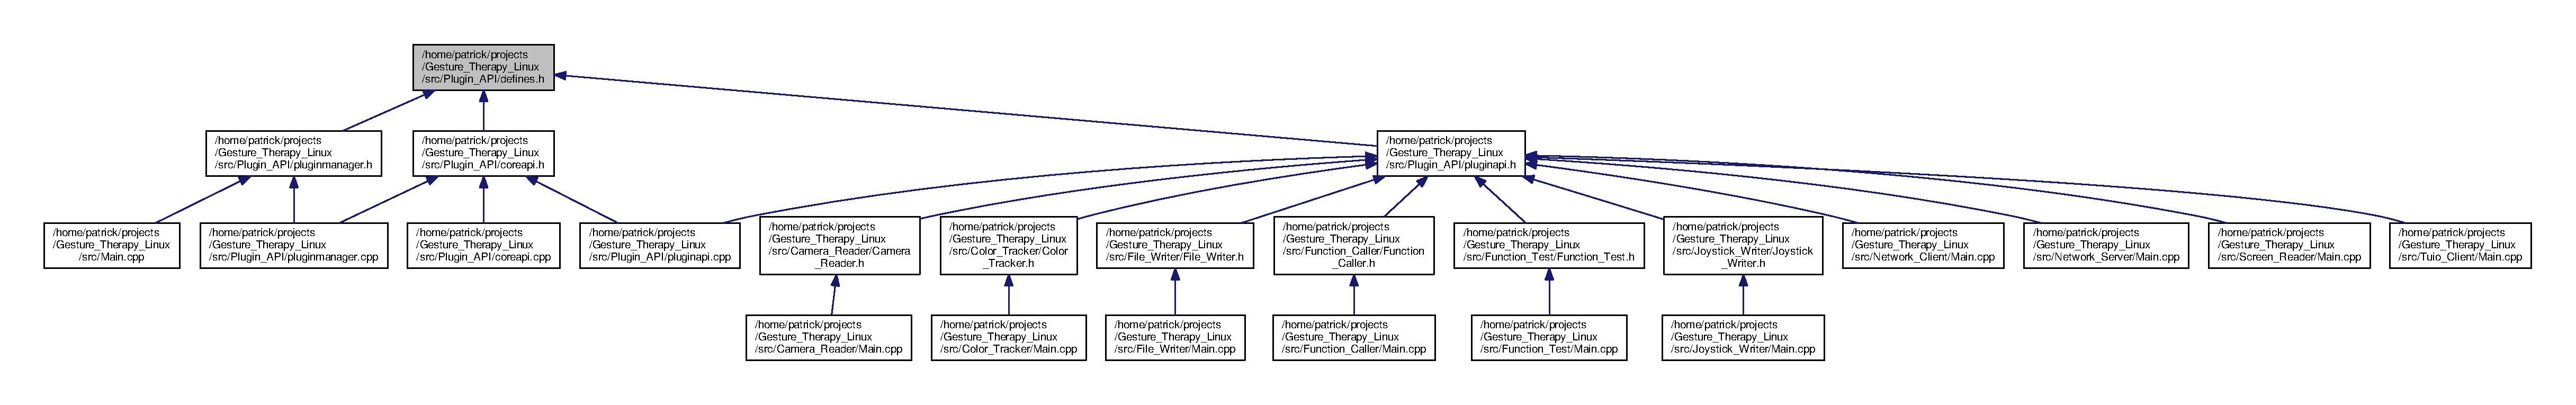
\includegraphics[width=350pt]{defines_8h__dep__incl}
\end{center}
\end{figure}


\subsection{Detailed Description}
Win32 decorator macros for the Core and Plugin A\+P\+Is. 

\begin{DoxyAuthor}{Author}
Patrick Heyer \href{mailto:patrickhey@prodigy.net.mx}{\tt patrickhey@prodigy.\+net.\+mx} 
\end{DoxyAuthor}

\hypertarget{plugin_8h}{}\section{/home/patrick/projects/\+Gesture\+\_\+\+Therapy\+\_\+\+Linux/src/\+Plugin\+\_\+\+A\+P\+I/plugin.h File Reference}
\label{plugin_8h}\index{/home/patrick/projects/\+Gesture\+\_\+\+Therapy\+\_\+\+Linux/src/\+Plugin\+\_\+\+A\+P\+I/plugin.\+h@{/home/patrick/projects/\+Gesture\+\_\+\+Therapy\+\_\+\+Linux/src/\+Plugin\+\_\+\+A\+P\+I/plugin.\+h}}
{\ttfamily \#include $<$string$>$}\newline
{\ttfamily \#include $<$iostream$>$}\newline
{\ttfamily \#include $<$pthread.\+h$>$}\newline
Include dependency graph for plugin.\+h\+:\nopagebreak
\begin{figure}[H]
\begin{center}
\leavevmode
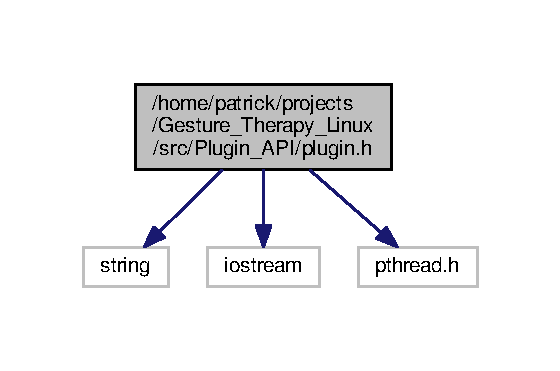
\includegraphics[width=269pt]{plugin_8h__incl}
\end{center}
\end{figure}
This graph shows which files directly or indirectly include this file\+:\nopagebreak
\begin{figure}[H]
\begin{center}
\leavevmode
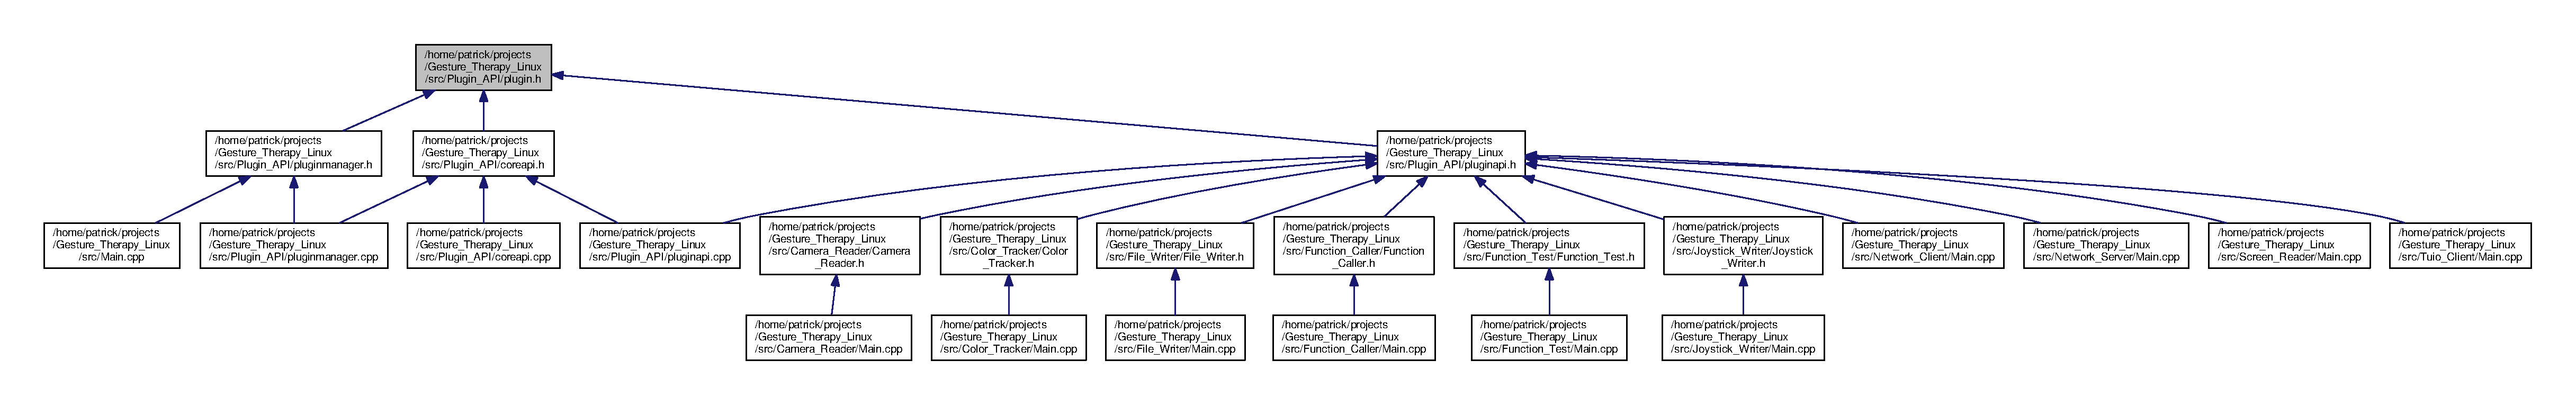
\includegraphics[width=350pt]{plugin_8h__dep__incl}
\end{center}
\end{figure}
\subsection*{Classes}
\begin{DoxyCompactItemize}
\item 
class \hyperlink{class_i_plugin}{I\+Plugin}
\end{DoxyCompactItemize}


\subsection{Detailed Description}
\begin{DoxyAuthor}{Author}
Patrick Heyer \href{mailto:patrickhey@prodigy.net.mx}{\tt patrickhey@prodigy.\+net.\+mx} 
\end{DoxyAuthor}

\hypertarget{pluginapi_8h}{}\section{/home/patrick/projects/\+Gesture\+\_\+\+Therapy\+\_\+\+Linux/src/\+Plugin\+\_\+\+A\+P\+I/pluginapi.h File Reference}
\label{pluginapi_8h}\index{/home/patrick/projects/\+Gesture\+\_\+\+Therapy\+\_\+\+Linux/src/\+Plugin\+\_\+\+A\+P\+I/pluginapi.\+h@{/home/patrick/projects/\+Gesture\+\_\+\+Therapy\+\_\+\+Linux/src/\+Plugin\+\_\+\+A\+P\+I/pluginapi.\+h}}


An A\+PI that lets users write plugins.  


{\ttfamily \#include \char`\"{}defines.\+h\char`\"{}}\newline
{\ttfamily \#include \char`\"{}plugin.\+h\char`\"{}}\newline
Include dependency graph for pluginapi.\+h\+:\nopagebreak
\begin{figure}[H]
\begin{center}
\leavevmode
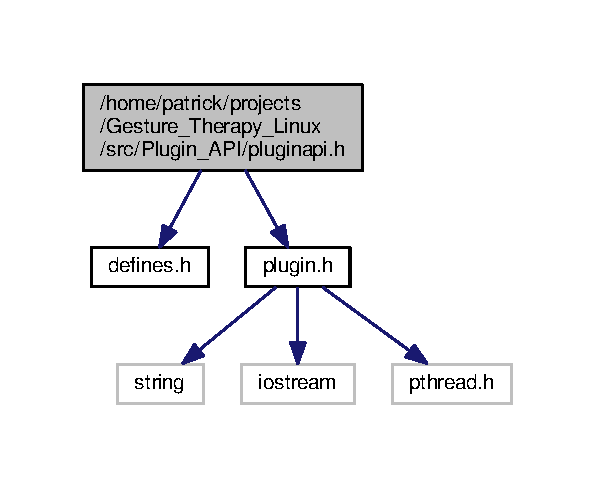
\includegraphics[width=286pt]{pluginapi_8h__incl}
\end{center}
\end{figure}
This graph shows which files directly or indirectly include this file\+:\nopagebreak
\begin{figure}[H]
\begin{center}
\leavevmode
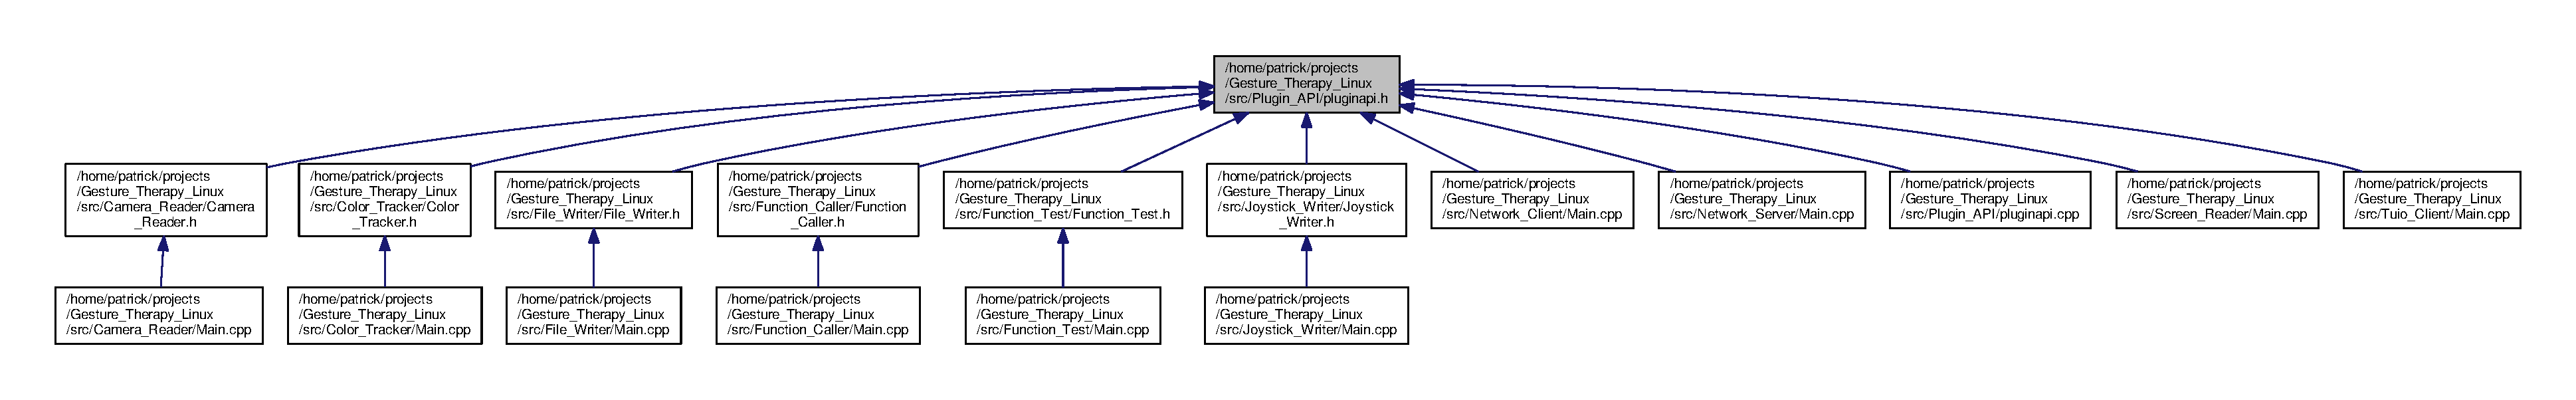
\includegraphics[width=350pt]{pluginapi_8h__dep__incl}
\end{center}
\end{figure}
\subsection*{Macros}
\begin{DoxyCompactItemize}
\item 
\mbox{\Hypertarget{pluginapi_8h_ac3bcb9217a74830c51b6c46c9b5f997f}\label{pluginapi_8h_ac3bcb9217a74830c51b6c46c9b5f997f}} 
\#define {\bfseries P\+L\+U\+G\+I\+N\+\_\+\+A\+P\+I\+\_\+\+V\+E\+R\+S\+I\+ON}~1
\item 
\mbox{\Hypertarget{pluginapi_8h_ada5e32e6261f8ecb0a75d6360a2d967c}\label{pluginapi_8h_ada5e32e6261f8ecb0a75d6360a2d967c}} 
\#define {\bfseries C\+O\+R\+E\+\_\+\+F\+U\+NC}~extern \char`\"{}C\char`\"{} C\+O\+R\+E\+\_\+\+A\+PI
\item 
\mbox{\Hypertarget{pluginapi_8h_a44d2700cebad9f4eb409e36bfe609ffb}\label{pluginapi_8h_a44d2700cebad9f4eb409e36bfe609ffb}} 
\#define {\bfseries P\+L\+U\+G\+I\+N\+\_\+\+F\+U\+NC}~extern \char`\"{}C\char`\"{} P\+L\+U\+G\+I\+N\+\_\+\+A\+PI
\item 
\#define \hyperlink{pluginapi_8h_a7a0dfe7f380fed1c658a9f1c2e66c910}{P\+L\+U\+G\+I\+N\+\_\+\+I\+N\+IT}()
\begin{DoxyCompactList}\small\item\em declare the initialization routine for a plugin \end{DoxyCompactList}\item 
\mbox{\Hypertarget{pluginapi_8h_a3a167eda0b8a7aa8854d62708a971a84}\label{pluginapi_8h_a3a167eda0b8a7aa8854d62708a971a84}} 
\#define \hyperlink{pluginapi_8h_a3a167eda0b8a7aa8854d62708a971a84}{P\+L\+U\+G\+I\+N\+\_\+\+F\+R\+EE}()~P\+L\+U\+G\+I\+N\+\_\+\+F\+U\+NC int Plugin\+Free()
\begin{DoxyCompactList}\small\item\em declare the cleanup routine for a plugin \end{DoxyCompactList}\item 
\mbox{\Hypertarget{pluginapi_8h_a1431b663bad20be0e123860f4977abf6}\label{pluginapi_8h_a1431b663bad20be0e123860f4977abf6}} 
\#define \hyperlink{pluginapi_8h_a1431b663bad20be0e123860f4977abf6}{P\+L\+U\+G\+I\+N\+\_\+\+D\+I\+S\+P\+L\+A\+Y\+\_\+\+N\+A\+ME}(name)~P\+L\+U\+G\+I\+N\+\_\+\+A\+PI const char $\ast$ Plugin\+Display\+Name = name
\begin{DoxyCompactList}\small\item\em declare the display name a plugin \end{DoxyCompactList}\item 
\mbox{\Hypertarget{pluginapi_8h_a3fa7c23fe803aced93676073abd6bb93}\label{pluginapi_8h_a3fa7c23fe803aced93676073abd6bb93}} 
\#define \hyperlink{pluginapi_8h_a3fa7c23fe803aced93676073abd6bb93}{P\+L\+U\+G\+I\+N\+\_\+\+D\+I\+S\+P\+L\+A\+Y\+\_\+\+T\+Y\+PE}(type)~P\+L\+U\+G\+I\+N\+\_\+\+A\+PI const char $\ast$ Plugin\+Type = type
\begin{DoxyCompactList}\small\item\em declare the type of a plugin I\+N\+P\+UT I\+N\+\_\+\+O\+UT O\+U\+T\+P\+UT \end{DoxyCompactList}\item 
\mbox{\Hypertarget{pluginapi_8h_ac1cb009f19f3d03f8c42fd5bc10fec5b}\label{pluginapi_8h_ac1cb009f19f3d03f8c42fd5bc10fec5b}} 
\#define \hyperlink{pluginapi_8h_ac1cb009f19f3d03f8c42fd5bc10fec5b}{P\+L\+U\+G\+I\+N\+\_\+\+M\+I\+N\+\_\+\+V\+E\+R\+S\+I\+ON}(version)~P\+L\+U\+G\+I\+N\+\_\+\+A\+PI const char $\ast$ Plugin\+Min\+Version = version
\begin{DoxyCompactList}\small\item\em declare the minimum required Plugin A\+PI version for a plugin \end{DoxyCompactList}\item 
\mbox{\Hypertarget{pluginapi_8h_a53cb1b274328eea11a979368bf873062}\label{pluginapi_8h_a53cb1b274328eea11a979368bf873062}} 
\#define \hyperlink{pluginapi_8h_a53cb1b274328eea11a979368bf873062}{P\+L\+U\+G\+I\+N\+\_\+\+M\+A\+X\+\_\+\+V\+E\+R\+S\+I\+ON}(version)~P\+L\+U\+G\+I\+N\+\_\+\+A\+PI const char $\ast$ Plugin\+Max\+Version = version
\begin{DoxyCompactList}\small\item\em declare the maximum supported Plugin A\+PI version for a plugin \end{DoxyCompactList}\end{DoxyCompactItemize}
\subsection*{Typedefs}
\begin{DoxyCompactItemize}
\item 
\mbox{\Hypertarget{pluginapi_8h_a246ac6d825804d6cb3f284a783fe1495}\label{pluginapi_8h_a246ac6d825804d6cb3f284a783fe1495}} 
typedef \hyperlink{class_i_plugin}{I\+Plugin} $\ast$($\ast$ \hyperlink{pluginapi_8h_a246ac6d825804d6cb3f284a783fe1495}{Plugin\+Init\+Func}) ()
\begin{DoxyCompactList}\small\item\em The function signature for a routine that creates a Plugin. \end{DoxyCompactList}\item 
\mbox{\Hypertarget{pluginapi_8h_ac55cc84b1f174f0cb9fcbe29ead2ce37}\label{pluginapi_8h_ac55cc84b1f174f0cb9fcbe29ead2ce37}} 
typedef void($\ast$ \hyperlink{pluginapi_8h_ac55cc84b1f174f0cb9fcbe29ead2ce37}{Plugin\+Free\+Func}) (\hyperlink{class_i_plugin}{I\+Plugin} $\ast$)
\begin{DoxyCompactList}\small\item\em The function signature for a routine that destroys a Plugin. \end{DoxyCompactList}\end{DoxyCompactItemize}
\subsection*{Functions}
\begin{DoxyCompactItemize}
\item 
\mbox{\Hypertarget{pluginapi_8h_ae5498706132ac40ada14c815d183ebfe}\label{pluginapi_8h_ae5498706132ac40ada14c815d183ebfe}} 
C\+O\+R\+E\+\_\+\+F\+U\+NC void \hyperlink{pluginapi_8h_ae5498706132ac40ada14c815d183ebfe}{Register\+Plugin} (const char $\ast$type, \hyperlink{pluginapi_8h_a246ac6d825804d6cb3f284a783fe1495}{Plugin\+Init\+Func} init\+\_\+cb, \hyperlink{pluginapi_8h_ac55cc84b1f174f0cb9fcbe29ead2ce37}{Plugin\+Free\+Func} free\+\_\+cb)
\begin{DoxyCompactList}\small\item\em A routine to let a plugin register a new Plugin type. \end{DoxyCompactList}\end{DoxyCompactItemize}


\subsection{Detailed Description}
An A\+PI that lets users write plugins. 

\begin{DoxyAuthor}{Author}
Patrick Heyer \href{mailto:patrickhey@prodigy.net.mx}{\tt patrickhey@prodigy.\+net.\+mx} 
\end{DoxyAuthor}


\subsection{Macro Definition Documentation}
\mbox{\Hypertarget{pluginapi_8h_a7a0dfe7f380fed1c658a9f1c2e66c910}\label{pluginapi_8h_a7a0dfe7f380fed1c658a9f1c2e66c910}} 
\index{pluginapi.\+h@{pluginapi.\+h}!P\+L\+U\+G\+I\+N\+\_\+\+I\+N\+IT@{P\+L\+U\+G\+I\+N\+\_\+\+I\+N\+IT}}
\index{P\+L\+U\+G\+I\+N\+\_\+\+I\+N\+IT@{P\+L\+U\+G\+I\+N\+\_\+\+I\+N\+IT}!pluginapi.\+h@{pluginapi.\+h}}
\subsubsection{\texorpdfstring{P\+L\+U\+G\+I\+N\+\_\+\+I\+N\+IT}{PLUGIN\_INIT}}
{\footnotesize\ttfamily \#define P\+L\+U\+G\+I\+N\+\_\+\+I\+N\+IT(\begin{DoxyParamCaption}{ }\end{DoxyParamCaption})}

{\bfseries Value\+:}
\begin{DoxyCode}
\textcolor{keyword}{const} \textcolor{keywordtype}{int} PluginVersion = PLUGIN\_API\_VERSION; \(\backslash\)
    PLUGIN\_FUNC \textcolor{keywordtype}{int} PluginInit()
\end{DoxyCode}


declare the initialization routine for a plugin 



Definition at line 20 of file pluginapi.\+h.


\hypertarget{pluginmanager_8h}{}\section{/home/patrick/projects/\+Gesture\+\_\+\+Therapy\+\_\+\+Linux/src/\+Plugin\+\_\+\+A\+P\+I/pluginmanager.h File Reference}
\label{pluginmanager_8h}\index{/home/patrick/projects/\+Gesture\+\_\+\+Therapy\+\_\+\+Linux/src/\+Plugin\+\_\+\+A\+P\+I/pluginmanager.\+h@{/home/patrick/projects/\+Gesture\+\_\+\+Therapy\+\_\+\+Linux/src/\+Plugin\+\_\+\+A\+P\+I/pluginmanager.\+h}}


A Plugin Manager singleton.  


{\ttfamily \#include \char`\"{}defines.\+h\char`\"{}}\newline
{\ttfamily \#include $<$string$>$}\newline
{\ttfamily \#include $<$vector$>$}\newline
{\ttfamily \#include $<$list$>$}\newline
{\ttfamily \#include $<$cstdlib$>$}\newline
{\ttfamily \#include \char`\"{}plugin.\+h\char`\"{}}\newline
Include dependency graph for pluginmanager.\+h\+:\nopagebreak
\begin{figure}[H]
\begin{center}
\leavevmode
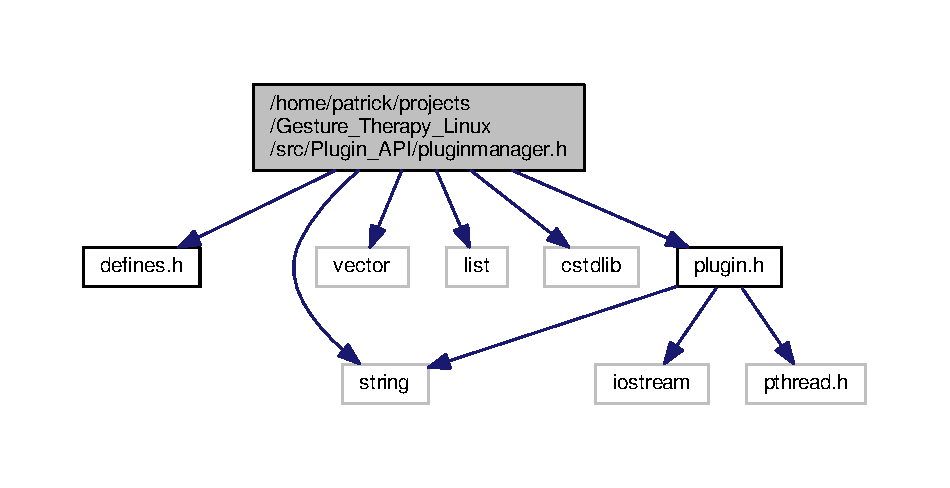
\includegraphics[width=350pt]{pluginmanager_8h__incl}
\end{center}
\end{figure}
This graph shows which files directly or indirectly include this file\+:\nopagebreak
\begin{figure}[H]
\begin{center}
\leavevmode
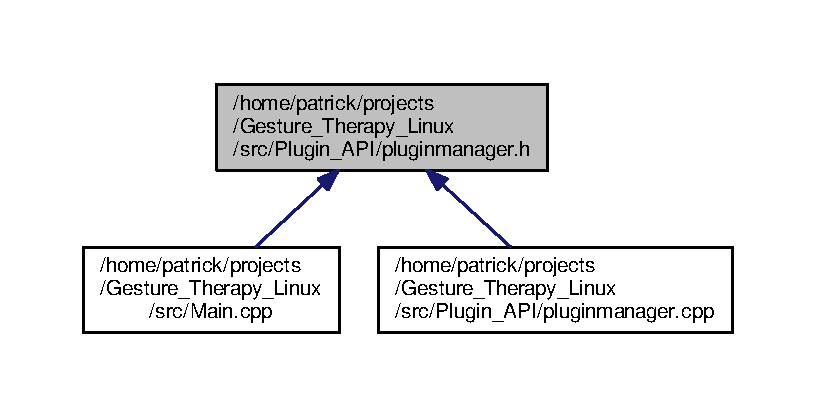
\includegraphics[width=350pt]{pluginmanager_8h__dep__incl}
\end{center}
\end{figure}
\subsection*{Classes}
\begin{DoxyCompactItemize}
\item 
class \hyperlink{class_plugin_instance}{Plugin\+Instance}
\begin{DoxyCompactList}\small\item\em C\+O\+R\+E\+\_\+\+A\+PI \hyperlink{class_plugin_instance}{Plugin\+Instance}. \end{DoxyCompactList}\item 
class \hyperlink{class_plugin_manager}{Plugin\+Manager}
\begin{DoxyCompactList}\small\item\em C\+O\+R\+E\+\_\+\+A\+PI \hyperlink{class_plugin_manager}{Plugin\+Manager}. \end{DoxyCompactList}\end{DoxyCompactItemize}


\subsection{Detailed Description}
A Plugin Manager singleton. 

\begin{DoxyAuthor}{Author}
Patrick Heyer \href{mailto:patrickhey@prodigy.net.mx}{\tt patrickhey@prodigy.\+net.\+mx} 
\end{DoxyAuthor}

%--- End generated contents ---

% Index
\backmatter
\newpage
\phantomsection
\clearemptydoublepage
\addcontentsline{toc}{chapter}{Index}
\printindex

\end{document}
